\documentclass[11pt]{article}
\usepackage[margin=1in]{geometry}
\usepackage{amsmath,amssymb,amsthm,mathtools}
\usepackage{enumitem}
\usepackage{graphicx}
\usepackage{hyperref}
\hypersetup{hidelinks,hypertexnames=false}
\usepackage{booktabs}
\usepackage{array}

\newtheorem{theorem}{Theorem}[section]
\newtheorem{lemma}[theorem]{Lemma}
\newtheorem{proposition}[theorem]{Proposition}
\newtheorem{corollary}[theorem]{Corollary}
\newtheorem{definition}[theorem]{Definition}

\newcommand{\Same}{\operatorname{Same}}
\newcommand{\Diff}{\operatorname{Diff}}
\newcommand{\Off}{\operatorname{Off}}
\newcommand{\calQ}{\mathcal Q}
\newcommand{\ind}{\mathbf 1}
\newcommand{\E}{\mathbb E}

\title{A Split-Decomposition Approach to the Bandelt--Dress Quartet Distance Bound}
\author{Libo Huang \and Stefan Gr\"unewald}
\date{}

\begin{document}
\maketitle


\begin{abstract}
Let $X$ be a set of $N$ taxa.  The quartet distance between two binary
leaf-labelled phylogenetic trees on $X$ counts the four-subsets on which the
two induced quartet trees differ.  Bandelt and Dress conjectured that its
maximum is asymptotic to
\[
\left(\frac23+o(1)\right)\binom N4.
\]
We prove the conjectured upper bound.  The argument has two stages.  First,
we form an auxiliary functional $f_1$ from squared $2\times2$ split
determinants and ordered-adjacent-edge corrections.  A local decomposition
uses row atoms $R_i$ and column atoms $C_k$.  Write
$a_{i,k}=|R_i\cap C_k|/N$, $c_k=|C_k|/N$, and let $C_{\bar k}$ denote the
opposite-side column block, with
$a_{i,\bar k}=|R_i\cap C_{\bar k}|/N$ and
$c_{\bar k}=|C_{\bar k}|/N$.  Every retained atom is nonempty, and the
opposite side of a relevant principal edge is nonempty; hence
$c_k,c_{\bar k}>0$.  The symmetric coefficient
\[
r_i^k=\frac12\left(\frac{a_{i,k}}{c_k}+\frac{a_{i,\bar k}}{c_{\bar k}}\right)
\]
reduces $f_1$ to four families of nonnegative quadratic forms.  The only
nonlocal step in this reduction is a bijective reversal of ordered
adjacent-edge bridges:
it exchanges the two endpoint blocks while preserving the middle block.

Second, we expand the same functional as a sum over $X^4$.  The resulting
antisymmetric kernel takes only the values $-1,0,1$.  The $24$ orderings of
a four-subset contribute $4$ if the two trees display the same quartet and
$-2$ otherwise, while all repeated-label tuples contribute $O(N^3)$.  Hence
writing $\Same(T_1,T_2)$ and $\Diff(T_1,T_2)$ for the numbers of four-subsets
on which the displayed quartets agree and differ, respectively,
\[
N^4f_1=4\Same(T_1,T_2)-2\Diff(T_1,T_2)+O(N^3),
\]
and $f_1\ge0$ yields the Bandelt--Dress bound.
\end{abstract}

\noindent\textbf{Keywords.} Quartet distance; phylogenetic tree; $X$-tree; split system; displayed quartet tree; Bandelt--Dress conjecture; nonnegative decomposition.

\noindent\textbf{Mathematics Subject Classification.} 05C05; 05C35; 92B10.

\section{Introduction}

Let $X$ be a finite set of taxa.  A binary leaf-labelled phylogenetic tree
on $X$ induces exactly one quartet tree on every four-subset of $X$.  The
quartet distance between two such trees is the number of four-subsets on
which these induced quartet trees differ.  It is a basic combinatorial
distance in phylogenetics.  We denote this number by
$\Diff(T_1,T_2)$ and put
$\Same(T_1,T_2):=\binom{|X|}{4}-\Diff(T_1,T_2)$.

We use the standard language of splits.  A split is a bipartition
$A\mid B$ of $X$, and it displays $ab\mid cd$ when $a,b$ lie on one side
and $c,d$ on the other.  Edge splits of a tree form a compatible split
system.  This viewpoint is also used in quartet reconstruction, QNet, and
weighted quartet systems
\cite{GrunewaldForslundDressMoulton2007,GrunewaldHuberMoultonSemple2008,Grunewald2010}.

For $N=|X|$, put
\[
M_N=\max_{T_1,T_2}\Diff(T_1,T_2),
\]
where the maximum is over all binary leaf-labelled phylogenetic trees on
$X$.  Bandelt and Dress introduced the symmetric quartet distance in their
work on reconstructing tree shape from dissimilarity data
\cite{BandeltDress1986}.  Their conjecture states that
\[
M_N\le \left(\frac23+o(1)\right)\binom N4.
\]
The matching lower bound follows by independently and uniformly labelling
two fixed binary tree shapes.  Alon, Naves and Sudakov proved the conjectured
upper bound for caterpillar trees and the general bound
$(0.69+o(1))\binom N4$ \cite{AlonNavesSudakov2016}.  A partial-information
version was studied in \cite{SnirWeissbergYuster2022}.

Our main result is the conjectured upper bound.  Equivalently, any two binary
leaf-labelled phylogenetic trees share at least
\[
\left(\frac13-o(1)\right)\binom N4
\]
displayed quartet trees.  More precisely, for $|X|=N$ we prove
\[
\frac{\Diff(T_1,T_2)}{\binom N4}\le \frac23+O\left(\frac1N\right).
\]
Together with the random-labelling lower bound this gives
\[
M_N=\left(\frac23+o(1)\right)\binom N4.
\]

The proof is organized around one auxiliary functional.  We first describe
the four steps of the argument; the definitions and calculations follow in
the subsequent sections.

\paragraph{1. Split determinants.}
Given two splits $P\mid P^c$ and $Q\mid Q^c$, consider their normalized
intersection table
\[
\begin{array}{c|cc}
&Q&Q^c\\
\hline
P&a&b\\
P^c&c&d
\end{array}
\]
The determinant square $(ad-bc)^2$ is a squared covariance of centered split
indicators.  We combine these squares into $f_1$.  Its four terms correspond
to using an ordinary edge split or an ordered-adjacent correction in each of
the two trees.  The coefficients $1,-1/2,-1/2,1/4$ correct the two orientation
multiplicities.

\paragraph{2. Local symmetric decomposition.}
A caterpillar has a linear order of adjacent intervals; a general tree does
not.  We replace that order by
\[
r_i^k=\frac12\left(\frac{a_{i,k}}{c_k}+\frac{a_{i,\bar k}}{c_{\bar k}}\right).
\]
Here $i$ is a row atom, $k$ is a column branch atom,
$a_{i,k}$ is their normalized intersection mass, $c_k$ is the mass of the
column atom, $k^+$ is its whole same-side block, and $\bar k$ is the
opposite-side block.  Only nonempty atoms are retained, and the principal
edge is relevant, so $c_k,c_{\bar k}>0$ and both displayed ratios are
defined.  The two coefficients $1/2$ are
algebraic symmetry weights.  They give
\[
\sum_i r_i^k=1
\]
where the sum ranges over all row atoms of the fixed chart,
and the coefficient bound
\[
4c_kc_l r_i^k r_j^l
\ge
\frac{c_kc_l}{c_{\bar k}c_{\bar l}}
a_{i,\bar k}a_{j,\bar l}.
\]
This inequality controls the negative terms left by the completion of squares.

\paragraph{3. Global bridge reversal and positivity.}
For a principal chart $\chi$ (a pair of relevant principal edges, formally
defined in Subsection~\ref{subsec:principal-charts}), denote the four
determinant levels by
$U_\chi,R_\chi,C_\chi,B_\chi$.  After multiplying by four, the expression to
be decomposed is
\[
4U_\chi-2R_\chi-2C_\chi+B_\chi.
\]
The row coordinate is decomposed while the column term is held fixed.  The
remaining column coefficients are grouped by the four-sector partition
defined in Subsection~\ref{subsec:local-four-sector}.
For an ordered adjacent edge pair, let $(K,H,L)$ denote, respectively, the
selected endpoint block, the middle block, and the opposite endpoint block
created by deleting the two edges.  Bridge reversal gives the different
principal chart with blocks $(L,H,K)$.  This fixed-point-free involution
matches the second endpoint square coefficient in each chart with the first
endpoint square coefficient in its reversed chart only after the complete
chart sum is taken.  The result is
\[
f_1=\sum_\chi\left(\frac14\mathcal S_{1,\chi}
+\frac12\mathcal S_{2,\chi}
+\frac12\mathcal S_{3,\chi}
+\mathcal S_{4,\chi}\right).
\]
Here $\mathcal S_{1,\chi},\ldots,\mathcal S_{4,\chi}$ denote the four
chart-indexed square-family polynomials declared explicitly in
Subsection~\ref{subsec:four-class-decomposition} and derived in
Appendix~\ref{app:local-expansion}.
The first two families are explicit sums of completed squares.  The last two
are squares multiplied by a coefficient $\Psi_{ij}^\chi(u)$; the displayed
coefficient bound proves that this multiplier is nonnegative.  Thus
$f_1\ge0$.

\paragraph{4. Quartet counting.}
Give every edge term weight $1$ and every ordered-adjacent correction weight
$-1/2$.  Their antisymmetric side-pair functions define a kernel $K_T$ on
$X^4$ satisfying
\[
 N^4f_1(T_1,T_2)=\frac14\sum_{\boldsymbol q\in X^4}
 K_{T_1}(\boldsymbol q)K_{T_2}(\boldsymbol q).
\]
For either positional pairing, the separating edges form an empty path or a
path of signed weight $1$.  This identifies
$K_T=\lambda_T(13\mid24)-\lambda_T(14\mid23)$ and hence
$K_T\in\{-1,0,1\}$, even when labels repeat.  Exactly
$6N^3-11N^2+6N$ ordered tuples contain a repeated label, and each contributes
at most $1/4$ in absolute value.  For each four-subset with distinct labels,
a direct count of its $24$ orderings gives total kernel contribution $4$ when
the displayed quartets agree and $-2$ when they differ.  Consequently
\[
 N^4f_1=4\Same(T_1,T_2)-2\Diff(T_1,T_2)+O(N^3).
\]
Since $f_1\ge0$, the desired quartet bound follows.

Sections 2--5 develop these four steps in order.  Section 6 explains the
scope of the result for general $X$-trees.  Appendix~\ref{app:local-expansion}
contains the coefficient calculation proving positivity;
Appendix~\ref{app:distance-covariance} records the related distance-covariance
identity; and Appendix~\ref{app:algorithmic-reverse-calculation} works through
the complete exact-arithmetic calculation for two non-caterpillar binary
trees.

\section{Preliminaries}

We distinguish the general objects needed for the local algebra from the
binary leaf-labelled trees to which the quartet-distance theorem applies.
Let $X$ be a finite set, $|X|=N$.  An \emph{$X$-tree} is a finite tree $T$
together with a vertex labelling
\[
v\in V(T)\longmapsto X_v\subseteq X
\]
such that the nonempty sets $X_v$ form a partition of $X$ and
$X_v\ne\varnothing$ whenever $v$ has degree at most two.  Thus a taxon may be
attached to an internal vertex, and a vertex may carry more than one taxon.
The condition on vertices of degree at most two is the usual reducedness
condition; in particular, every leaf carries a taxon, so deleting any edge
produces two nonempty taxon sets.

A \emph{leaf-labelled phylogenetic tree on $X$} is the special case in which
each nonempty $X_v$ is a singleton and the labelled vertices are exactly the
leaves.  In the main theorem the tree has no degree-two vertices and is
\emph{binary}, meaning that every internal vertex has degree three.  The
coefficient calculation is written for the more general $X$-tree notation,
but the quartet-counting conclusion is used only in this binary
leaf-labelled setting.

For a leaf-labelled tree and $Y\subseteq X$, let $T|Y$ denote the tree obtained from the minimal subtree of $T$ connecting the leaves labelled by $Y$ by suppressing all unlabelled degree-two vertices.  If $|Y|=4$ and $T$ is binary, then $T|Y$ is a quartet tree.  We write $ab\mid cd$ for the quartet tree in which the path from $a$ to $b$ is edge-disjoint from the path from $c$ to $d$.

A \emph{split} of $X$ is a bipartition $A\mid B$ with $A,B\ne\varnothing$.  We usually write $B=A^c$.  Every edge $e$ of an $X$-tree induces a split $\sigma_e=A_e\mid A_e^c$ by deleting $e$: the two components of $T-e$ carry the taxa in $A_e$ and $A_e^c$, respectively.  In the leaf-labelled case this is the usual edge split.  The set
\[
\Sigma(T)=\{\sigma_e:e\in E(T)\}
\]
is the split system associated with $T$.  We also use the quartet-relevant edge set
\[
E_2(T)=\{e\in E(T): |A_e|\ge 2 \text{ and } |A_e^c|\ge 2\},
\]
and the corresponding quartet-relevant split system
\[
\Sigma_2(T)=\{\sigma_e:e\in E_2(T)\}.
\]

Only splits in $\Sigma_2(T)$ can display a resolved quartet tree on four distinct taxa.  A split $A\mid B$ \emph{displays} a quartet tree $ab\mid cd$ if $a,b\in A$ and $c,d\in B$, or vice versa.

Let $\calQ(X)$ be the set of quartet trees with leaf set a four-subset of $X$.  A binary leaf-labelled phylogenetic tree $T$ displays the quartet set
\[
\calQ(T)=\{T|Y:Y\in \binom X4\}\subseteq \calQ(X).
\]
For two binary leaf-labelled phylogenetic trees $T_1,T_2$, define
\[
\Same(T_1,T_2)=|\calQ(T_1)\cap \calQ(T_2)|
\]
and
\[
\Diff(T_1,T_2)=\binom N4-\Same(T_1,T_2).
\]
Equivalently, $\Diff(T_1,T_2)$ is the number of four-subsets $Y\in\binom X4$ for which $T_1|Y\ne T_2|Y$.

\section{Split determinants and the auxiliary functional}

This section constructs $f_1$ in three steps.  We first associate a
nonnegative determinant square with two splits, then extend the same formula
to the side-pairs obtained from adjacent edges, and finally combine the four
ordinary/corrected choices in the two tree coordinates.

\subsection{One pair of splits}

Let
\[
\sigma=P\mid P^c,
\qquad
\tau=Q\mid Q^c
\]
be two splits of $X$.  Define the normalized $2\times2$ table
\[
\begin{array}{c|cc}
&Q&Q^c\\
\hline
P&a&b\\
P^c&c&d
\end{array}
\]
where
\[
a=\frac{|P\cap Q|}{N},\quad
b=\frac{|P\cap Q^c|}{N},\quad
c=\frac{|P^c\cap Q|}{N},\quad
d=\frac{|P^c\cap Q^c|}{N}.
\]
Set
\[
D(\sigma,\tau)=(ad-bc)^2.
\]
This determinant square is the leading normalized contribution of the pair of splits to the expression $4\Same-2\Diff$.

\subsection{Indicator form of the split determinant}

We use the uniform probability measure on $X$.  For $A\subseteq X$, let
\[
\ind_A(x)=
\begin{cases}
1,&x\in A,\\
0,&x\notin A,
\end{cases}
\qquad
\mu(A)=\E\ind_A=\frac{|A|}{N},
\]
and put
\[
z_A=\ind_A-\mu(A).
\]
For a logical condition $\mathsf P$, we also use
$\mathbf 1_{\mathsf P}\in\{0,1\}$ for its truth indicator.  This scalar
notation is used later to turn endpoint or residual cases on and off.
For a split $\sigma=A\mid A^c$, replacing $A$ by $A^c$ changes $z_A$ to $-z_A$.  Hence the square of any inner product involving $z_A$ is independent of the chosen side of the split.

For $\sigma=P\mid P^c$ and $\tau=Q\mid Q^c$, a direct calculation gives
\[
\E z_Pz_Q
=
\E(\ind_P-a-b)(\ind_Q-a-c)
=a-(a+b)(a+c).
\]
Using $a+b+c+d=1$, this becomes
\[
a-(a+b)(a+c)=a(1-a-b-c)-bc=ad-bc.
\]
Therefore
\[
D(\sigma,\tau)=\left(\E z_Pz_Q\right)^2.
\]
The expression is unchanged if one reverses either split, because this only
changes the sign of the corresponding centered indicator.

Thus the local determinant is a squared covariance.  The role of the
adjacent-pair terms is not to change this basic quantity, but to combine it
across neighboring edges in a way that both admits a nonnegative
decomposition and counts each displayed quartet with the desired weight.


\subsection{Adjacent-pair correction operator}\label{subsec:adjacent-pair-correction}

Let $E(\mathcal T)$ denote the edge set of a tree $\mathcal T$.  For
$e,e'\in E(\mathcal T)$, write $e\sim e'$ if the two edges are adjacent.  Let
\[
\overrightarrow A_2(\mathcal T)
=\{(e,e')\in E_2(\mathcal T)^2:e\sim e'\}
\]
be the set of ordered adjacent pairs of quartet-relevant edges.

We now define the adjacent correction.  A \emph{side-pair} is an ordered pair
$(A,B)$ of disjoint nonempty subsets of $X$; unlike a split, it need not cover
$X$.  For two side-pairs $(A,B)$ and $(C,D)$ define
\[
T[(A,B),(C,D)]
:=\left(
\frac{|A\cap C|}{N}\frac{|B\cap D|}{N}
-
\frac{|A\cap D|}{N}\frac{|B\cap C|}{N}
\right)^2.
\]
Reversing either side-pair only changes the sign of the determinant before squaring.  If $A\cup B=X$ and $C\cup D=X$, this is the ordinary split determinant $D(A\mid B,C\mid D)$.

Let $(e,e')\in\overrightarrow A_2(\mathcal T)$, and let $v$ be the common
endpoint of $e$ and $e'$.  Removing the two adjacent edges gives three taxa
blocks.  Let $K_{e,e'}$ be the component beyond $e'$ away from $v$, and let
$L_{e,e'}$ be the component beyond $e$ away from $v$.  The adjacent-pair
correction $C_{e,e'}$ is the side-pair
\[
C_{e,e'}:=(K_{e,e'},L_{e,e'}).
\]
Thus, for a split $\tau=Q\mid Q^c$ in a second tree,
\[
T[C_{e,e'},\tau]:=T[(K_{e,e'},L_{e,e'}),(Q,Q^c)],
\]
and the definitions of $T[\sigma,C_{f,f'}]$ and $T[C_{e,e'},C_{f,f'}]$ are analogous.  In the local cluster notation of Appendix~\ref{app:local-expansion}, this side-pair determinant is exactly the neighboring contrast squared in equation~\eqref{eq:A18}; equations~\eqref{eq:A20}--\eqref{eq:A25} then expand and complete its mixed coefficient.

Indeed, let $C_{e,e'}=(K,L)$ and let $\tau=Q\mid Q^c$.  Put
\[
A=\frac{|K\cap Q|}{N},\qquad C=\frac{|L\cap Q|}{N},
\qquad c_K=\frac{|K|}{N},\qquad c_L=\frac{|L|}{N}.
\]
For the centered split-side indicator $Z=z_Q$, one has
\[
x_{Z,K}=A-c_K\mu(Q),\qquad x_{Z,L}=C-c_L\mu(Q).
\]
Therefore
\[
\begin{aligned}
T[(K,L),(Q,Q^c)]
&=\bigl(A(c_L-C)-(c_K-A)C\bigr)^2\\
&=(c_LA-c_KC)^2
=(c_Kx_{Z,L}-c_Lx_{Z,K})^2.
\end{aligned}
\]
Thus the side-pair determinant is precisely the local neighboring contrast used in Appendix~\ref{app:local-expansion}.

For four distinct taxa, the adjacent side-pair has the expected quartet
indicator $I_{C_{e,e'}}^\pi=I_e^\pi I_{e'}^\pi$.  The counting argument
requires the positional version of this identity on all of $X^4$, including
repeated labels.  That version, with every indicator defined explicitly, is
proved in Lemma~\ref{lem:full-domain-correction-indicator}.

For an edge $e\in E_2(\mathcal T)$, define the one-sided adjacent correction by
\[
T[\sigma_e^+,\tau]
:=\sum_{e':\,(e,e')\in\overrightarrow A_2(\mathcal T)}
T[C_{e,e'},\tau].
\]
For $e\in E_2(T_1)$ and $f\in E_2(T_2)$, the remaining plus notations mean
formal sums over indexed occurrences:
\[
\begin{aligned}
T[\sigma,\tau_f^+]
&:=\sum_{f':\,(f,f')\in\overrightarrow A_2(T_2)}
T[\sigma,C_{f,f'}],\\
T[\sigma_e^+,\tau_f^+]
&:=\sum_{e':\,(e,e')\in\overrightarrow A_2(T_1)}
\sum_{f':\,(f,f')\in\overrightarrow A_2(T_2)}
T[C_{e,e'},C_{f,f'}].
\end{aligned}
\]
Thus every determinant is squared before the indexed occurrences are summed;
no linearity of the squared determinant itself is being asserted.  This is the
convention used throughout the paper for neighboring corrections.

\begin{definition}[Auxiliary functional]
Define the auxiliary functional by summing only over quartet-relevant edge splits:
\[
\begin{aligned}
f_1(T_1,T_2)
&=
\sum_{e\in E_2(T_1)}\sum_{f\in E_2(T_2)}
\bigg(
T[\sigma_e,\tau_f]
-
\frac12T[\sigma_e^+,\tau_f]
-
\frac12T[\sigma_e,\tau_f^+]\\
&\hspace{3.5cm}
+
\frac14T[\sigma_e^+,\tau_f^+]
\bigg),
\end{aligned}
\]
where $\sigma_e$ and $\tau_f$ are the splits induced by $e$ and $f$, and
where adjacent-pair corrections are taken over
$\overrightarrow A_2(T_1)$ and $\overrightarrow A_2(T_2)$.  Splits with a
side of size one---and hence pendant splits in the binary leaf-labelled
setting---are excluded because they cannot display a quartet tree on four
distinct taxa.
\end{definition}

The coefficients $1/2$ and $1/4$ are purely combinatorial.  Each unordered adjacent pair has two
orientations, which gives $1/2$ for a correction in one tree and $1/4$ when
both tree coordinates are corrected.

\subsection[Reduction to the E2-core]{Reduction to the $E_2$-core}

The local argument depends only on quartet-relevant edges and their adjacent
side-pairs.  The following reduction removes the remaining parts of the trees
without changing these data.

\begin{lemma}[$E_2$-core contraction]\label{lem:E2-core-contraction}
Let $T$ be an $X$-tree and suppose that $E_2(T)\ne\varnothing$.  Let $K_2(T)$ be
the subgraph whose edges are those in $E_2(T)$ and whose vertices are their
endpoints.  Then $K_2(T)$ is a connected subtree.  Contract every component of
$T-V(K_2(T))$, together with its unique incident edge to $K_2(T)$, to its attachment
vertex, and transfer all taxa in that component to the attachment vertex.
Denote the resulting $X$-tree by $T^\circ$.  Then:
\begin{enumerate}[label=\textup{(\roman*)}]
\item under the natural identification, $E(T^\circ)=E_2(T)$, and the
      adjacency relations among these edges are unchanged;
\item every split induced by an edge $e\in E_2(T)$ is unchanged as a split of
      $X$;
\item every adjacent side-pair $C_{e,e'}$, with
      $(e,e')\in\overrightarrow A_2(T)$, is unchanged;
\item replacing either argument of $f_1$ by its $E_2$-core contraction does
      not change $f_1$; in particular,
      \[
      f_1(T_1,T_2)=f_1(T_1^\circ,T_2^\circ)
      \]
      whenever both contractions are defined.
\end{enumerate}
In the chart notation formalized in
Subsection~\ref{subsec:principal-charts}, the endpoint classes $a_e$ and
$b_e$ index the adjacent $E_2$-directions.  The atom belonging to one such
direction contains every taxon lying beyond that adjacent core edge,
including taxa transferred to more distant core vertices in the same
branch.  Only taxa located at an endpoint of $e$ after contraction (whether
already there or transferred there) and lying beyond no adjacent
$E_2$-direction enter the residual vertex classes $c_e$ and $d_e$.
\end{lemma}

\begin{proof}
Let $e,g\in E_2(T)$, and let $h$ be an edge on the path from $e$ to $g$.
One component of $T-h$ contains the side of $e$ directed away from $h$ and
therefore contains at least two taxa.  The other contains the corresponding
side of $g$ and also contains at least two taxa.  Hence $h\in E_2(T)$, so the
edges in $E_2(T)$ form the connected subtree $K_2(T)$.

Every component of $T-V(K_2(T))$ has a unique attachment vertex in $K_2(T)$;
otherwise the path between two attachment vertices would contain an edge
outside $E_2(T)$.  Contracting such a component moves taxa only within a
single component of $T-e$ for each $e\in E_2(T)$.  Thus the two taxon sets of
every $E_2$-split are unchanged, proving \textup{(ii)}.  By construction every
edge outside $K_2(T)$ is contracted, while no edge of $K_2(T)$ and no two
distinct core vertices are identified.  Hence $E(T^\circ)=E_2(T)$, and two
surviving edges are adjacent in $T^\circ$ exactly when they were adjacent in
$T$, proving \textup{(i)}.

The contracted tree is again reduced.  Indeed, let $v$ be a vertex whose
degree in $T^\circ$ is at most two.  If no edge incident with $v$ was
contracted, then its degree in $T$ was already at most two, so $v$ carried a
taxon by reducedness of $T$.  Otherwise at least one component attached to
$v$ was contracted onto $v$.  Every such component contains a taxon: an edge
joining it to the core separates a nonempty taxon set from the rest of $X$,
as every edge of an $X$-tree does.  Those taxa are transferred to $v$.
Hence every vertex of degree at most two in $T^\circ$ carries a nonempty
label set, as required.

For adjacent core edges $e,e'$, each contracted component was already
contained in one of the three taxon blocks obtained by deleting $e$ and $e'$.
The side-pair $C_{e,e'}$ is therefore unchanged, proving \textup{(iii)}.
Since the definition of $f_1$ uses only the $E_2$-splits and these ordered
adjacent side-pairs, \textup{(iv)} follows.  The final statement follows from
the construction of the contracted chart.
\end{proof}

If $E_2(T_1)=\varnothing$ or $E_2(T_2)=\varnothing$, every term in the
definition of $f_1(T_1,T_2)$ is absent and hence $f_1(T_1,T_2)=0$.  The
nonnegativity statement is then immediate.  In the remainder of the local
proof we therefore assume that both $E_2$-cores are nonempty and work with
$T_1^\circ$ and $T_2^\circ$.

\section{Symmetric decomposition and local nonnegativity}

The goal of this section is to reduce $f_1\ge0$ to a finite coefficient
inequality.  Throughout this section and
Appendix~\ref{app:local-expansion}, a \emph{relevant edge} means an edge in
the quartet-relevant set $E_2$ of the contracted core under discussion.  A
pair of relevant edges $(e,f)$, one from each tree, determines a
\emph{principal chart}.  Each edge is surrounded by endpoint atoms, which
index adjacent corrections, and possible residual atoms, which do not.  We
use the following convention throughout the local calculation:
\[
\begin{array}{c|c|c}
\text{symbol}&\text{coordinate}&\text{meaning}\\
\hline
e,f&\text{tree edges}&\text{principal edges of the chart}\\
i,j&\text{row copy}&\text{atoms around }e\\
k,l,u&\text{column copy}&\text{atoms around }f\\
a,b&\text{either copy}&\text{endpoint atoms indexing adjacent edges}\\
c,d&\text{either copy}&\text{residual atoms at the two endpoints}
\end{array}
\]
The construction below first defines these objects, then proves the one
coefficient inequality needed in Appendix~\ref{app:local-expansion}.

\subsection{Principal charts}\label{subsec:principal-charts}

We use the $E_2$-core contractions from
Lemma~\ref{lem:E2-core-contraction}.  Let $T^\circ$ be such a contraction and
let $e=\{v_-,v_+\}\in E_2(T^\circ)$.  Orient $e$ from $v_-$ to $v_+$ only to
name its two sides, and let $X_e^-$ and $X_e^+$ be the taxon sets in the two
components of $T^\circ-e$.  If
$g\in E_2(T^\circ)\setminus\{e\}$ is incident with $v_-$, let $A_e(g)$ be the
taxa in the component beyond $g$ away from $v_-$.  Define $A_e(g)$
analogously for edges incident with $v_+$.  The residual vertex blocks are
\[
 V_e^-:=X_e^-\setminus\bigsqcup_{\substack{
 g\in E_2(T^\circ)\setminus\{e\},\ g\sim e\\g\ni v_-}}A_e(g),
 \qquad
 V_e^+:=X_e^+\setminus\bigsqcup_{\substack{
 g\in E_2(T^\circ)\setminus\{e\},\ g\sim e\\g\ni v_+}}A_e(g).
\]
After empty residual blocks are omitted, these sets form the atom partition
\[
 \Pi_e=
 \{A_e(g):g\in E_2(T^\circ),\ g\sim e\}
 \sqcup\{V_e^-,V_e^+\}_{\ne\varnothing}.
\]
The atoms $A_e(g)$ at $v_-$ and $v_+$ form the endpoint classes $a_e$ and
$b_e$, respectively; the possible blocks $V_e^-$ and $V_e^+$ form $c_e$ and
$d_e$.  Thus endpoint atoms are indexed by ordered adjacent pairs $(e,g)$,
whereas residual atoms do not index adjacent corrections.

Let $\Omega_e$ index the nonempty atoms of $\Pi_e$; thus
$a_e,b_e,c_e,d_e\subseteq\Omega_e$ are the four atom-index classes just
described.  When this partition belongs to the first tree, write
$\Omega_e^{\rm r}$ for its row-labelled copy, and when it belongs to the
second tree, write $\Omega_e^{\rm c}$ for its column-labelled copy.  The
superscripts distinguish chart copies and do not alter the underlying atom
partition.

For two contracted trees, a principal chart is simply a pair
\[
 \chi=(e,f)\in E_2(T_1^\circ)\times E_2(T_2^\circ).
\]
Write
\[
 \Omega_{\rm r}^\chi:=\Omega_e^{\rm r},\qquad
 \Omega_{\rm c}^\chi:=\Omega_f^{\rm c},
\]
and write $R_i^\chi$ and $C_k^\chi$ for the corresponding row and column
taxon atoms.  For $P\subseteq\Omega_{\rm r}^\chi$ and
$Q\subseteq\Omega_{\rm c}^\chi$, put
\[
 R_P^\chi:=\bigsqcup_{i\in P}R_i^\chi,\qquad
 C_Q^\chi:=\bigsqcup_{k\in Q}C_k^\chi.
\]
For the column copy, set $a^\chi:=a_f$, $b^\chi:=b_f$,
$c^\chi:=c_f$, and $d^\chi:=d_f$.  For every
$k\in\Omega_{\rm c}^\chi$, define its same-side block, same-side aggregate,
and opposite-side block by
\[
 S_\chi(k):=
 \begin{cases}
 a^\chi\cup c^\chi,&k\in a^\chi\cup c^\chi,\\
 b^\chi\cup d^\chi,&k\in b^\chi\cup d^\chi,
 \end{cases}
 \qquad
 k^{+,\chi}:=S_\chi(k),\qquad
 \bar k_\chi:=\Omega_{\rm c}^\chi\setminus S_\chi(k).
\]
When the chart is fixed, we suppress the chart decoration.  If $k$ is an
endpoint atom corresponding to an edge $g$ adjacent to $f$, the ordered bridge
$\alpha=(f,g)$ has three taxon blocks
\[
 K_\alpha=C_k^\chi,\qquad
 H_\alpha=C_{k^{+,\chi}\setminus\{k\}}^\chi,\qquad
 L_\alpha=C_{\bar k_\chi}^\chi.
\]
Its reversal $\rho\alpha=(g,f)$ belongs to the different principal chart
$\rho\chi=(e,g)$ and has selected, middle, and opposite blocks
$(L_\alpha,H_\alpha,K_\alpha)$.  Thus reversal is a fixed-point-free
involution of the complete ordered endpoint-chart range.  In particular, it
does not mean replacing $k$ by the aggregate $\bar k$ inside a single chart.

Every sum over $a_e\cup b_e$ therefore ranges over atom indices associated
with adjacent directions in $E_2(T^\circ)$.  An endpoint atom may contain
taxa transferred to any more distant core vertex in its branch.  The
residual blocks $c_e\cup d_e$ contain only the taxa located at the two
endpoints of $e$ that lie beyond no such adjacent direction.  These
residual classes may be nonempty even when the original tree is binary and
leaf-labelled.

\subsection{Local notation}

Fix a principal chart $\chi=(e,f)$ and suppress $\chi$ from the notation.
Let the local clusters induced by the split of $e$ be indexed by $i,j$, and
those induced by the split of $f$ be indexed by $k,l$.  Write
\[
r_i=\frac{|R_i|}{N},
\qquad
c_k=\frac{|C_k|}{N},
\qquad
a_{i,k}=\frac{|R_i\cap C_k|}{N}.
\]
Let
\[
x_{i,k}=a_{i,k}-r_ic_k.
\]
Then
\[
\sum_i r_i=1,\qquad \sum_k c_k=1,
\]
\[
\sum_i a_{i,k}=c_k,\qquad \sum_k a_{i,k}=r_i,
\]
and hence
\[
\sum_i x_{i,k}=0,
\qquad
\sum_k x_{i,k}=0.
\]

For a local column index $k$, the blocks $k^+=S_\chi(k)$ and
$\bar k=\Omega_{\rm c}^\chi\setminus S_\chi(k)$ are the same-side and
opposite-side blocks defined in the preceding subsection.  More generally,
for any block $U$ of local column indices, use the additive notation
\[
c_U=\sum_{l\in U}c_l,
\qquad
a_{i,U}=\sum_{l\in U}a_{i,l},
\qquad
x_{i,U}=\sum_{l\in U}x_{i,l}.
\]
These are respectively the mass, mixed mass, and centered mass of the union of
the column clusters indexed by $U$; in particular this convention applies to
$U=\bar k$.
We assume $c_k>0$ and $c_{\bar k}>0$; zero-mass indices contribute nothing and may be omitted.

\subsection{The side-reversal symmetric decomposition}

For each $k$, set
\[
r_i^k=\frac12\left(\frac{a_{i,k}}{c_k}+\frac{a_{i,\bar k}}{c_{\bar k}}\right).
\]

This is the equal algebraic average associated with the taxon side-pair
$(C_k,C_{\bar k})$; it is not a mass-weighted average over the two blocks.
When $k$ is an endpoint atom, exchanging the two taxon blocks is realized by
the global bridge-reversal reindexing to the reversed principal chart.  For a
residual atom the formula is only a same-side/opposite-side algebraic average;
no reversed endpoint chart is asserted.  For each fixed $k$,
\[
\sum_i r_i^k
=
\frac12\left(
\frac{\sum_i a_{i,k}}{c_k}
+
\frac{\sum_i a_{i,\bar k}}{c_{\bar k}}
\right)
=
\frac12\left(\frac{c_k}{c_k}+\frac{c_{\bar k}}{c_{\bar k}}\right)=1.
\]

\begin{lemma}[Domination generated by the decomposition]\label{lem:domination-basic}
For any $i,j,k,l$,
\[
\begin{aligned}
4c_kc_l r_i^k r_j^l
&=
a_{i,k}a_{j,l}
+
\frac{c_l}{c_{\bar l}}a_{i,k}a_{j,\bar l}
+
\frac{c_k}{c_{\bar k}}a_{i,\bar k}a_{j,l}\\
&\quad+
\frac{c_kc_l}{c_{\bar k}c_{\bar l}}a_{i,\bar k}a_{j,\bar l}.
\end{aligned}
\]
In particular,
\[
4c_kc_l r_i^k r_j^l
\ge
\frac{c_kc_l}{c_{\bar k}c_{\bar l}}a_{i,\bar k}a_{j,\bar l}.
\]
\end{lemma}

\begin{proof}
Expanding the definition gives
\[
\begin{aligned}
4c_kc_l r_i^k r_j^l
&=
c_kc_l
\left(\frac{a_{i,k}}{c_k}+\frac{a_{i,\bar k}}{c_{\bar k}}\right)
\left(\frac{a_{j,l}}{c_l}+\frac{a_{j,\bar l}}{c_{\bar l}}\right)\\
&=
a_{i,k}a_{j,l}
+
\frac{c_l}{c_{\bar l}}a_{i,k}a_{j,\bar l}
+
\frac{c_k}{c_{\bar k}}a_{i,\bar k}a_{j,l}
+
\frac{c_kc_l}{c_{\bar k}c_{\bar l}}a_{i,\bar k}a_{j,\bar l}.
\end{aligned}
\]
All terms on the right are nonnegative.
\end{proof}

\subsection{Index sets for the local configuration}
\label{subsec:local-four-sector}

We now fix the local four-sector data used in the coefficient calculation.  The proof uses only the following finite combinatorial structure.  There is a finite index set $\Omega$ together with a disjoint decomposition
\[
\Omega=a\sqcup b\sqcup c\sqcup d.
\]
Here $a,b,c,d$ are four \emph{sets of atom indices}; they are not the scalar
entries denoted by the same letters in the earlier $2\times2$ contingency
table.  In a principal chart $\chi=(e,f)$ this generic partition is
instantiated separately in the two coordinates:
\[
\begin{aligned}
(a_{\rm r}^\chi,b_{\rm r}^\chi,c_{\rm r}^\chi,d_{\rm r}^\chi)
&=(a_e,b_e,c_e,d_e),\\
(a_{\rm c}^\chi,b_{\rm c}^\chi,c_{\rm c}^\chi,d_{\rm c}^\chi)
&=(a_f,b_f,c_f,d_f).
\end{aligned}
\]
The subscripts ${\rm r}$ and ${\rm c}$ are mandatory whenever both copies
occur in one calculation; the undecorated letters are used only for one fixed
copy.
This decomposition determines two same-side blocks,
\[
S_L:=a\cup c,
\qquad
S_R:=b\cup d.
\]
In the local $X$-tree interpretation, the classes $a$ and $b$ index ordinary incident branch classes at the two endpoints of the central local edge, while $c$ and $d$ index taxa blocks carried by the two endpoint vertices themselves.  No particular cardinalities are assumed; the argument below uses only the partition of $\Omega$ and the same-side relation determined by $S_L$ and $S_R$.

\begin{figure}[htbp]
\centering
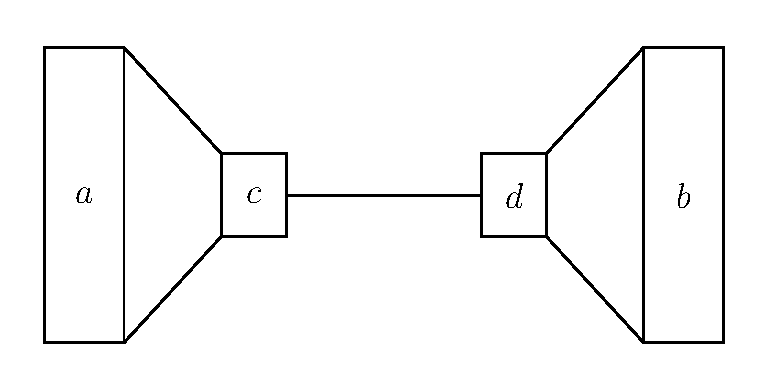
\includegraphics[width=0.422\textwidth]{local_four_sector_vector.pdf}
\caption{The local four-sector configuration used to define the index sets.
From left to right the four displayed blocks are $a,c,d,b$; hence the two
same-side blocks are $a\cup c$ and $b\cup d$.}
\label{fig:local-four-sector}
\end{figure}

With the two same-side blocks shown in Figure~\ref{fig:local-four-sector}, let
$S(k)$ denote the same-side block containing $k\in\Omega$:
\[
S(k)=
\begin{cases}
S_L,& k\in S_L,\\
S_R,& k\in S_R.
\end{cases}
\]
We set
\[
k^+:=S(k),
\qquad
\bar k:=\Omega\setminus S(k).
\]
Thus $k^+$ is the whole same-side block containing $k$, whereas $\bar k$ is the opposite-side block.  In particular, $\bar k$ is a block of indices, not a second singleton index.


\subsection{The exact four-class decomposition}
\label{subsec:four-class-decomposition}

For a principal chart $\chi=(e,f)$, write
\[
 U_\chi=T[\sigma_e,\tau_f],\qquad
 R_\chi=T[\sigma_e^+,\tau_f],\qquad
 C_\chi=T[\sigma_e,\tau_f^+],\qquad
 B_\chi=T[\sigma_e^+,\tau_f^+].
\]
Before declaring the four square families, define their row relation sets.
Put
\[
\mathcal E_{\rm r}^\chi:=a_{\rm r}^\chi\cup b_{\rm r}^\chi,\qquad
\Delta_{\mathcal E_{\rm r}^\chi}
:=\{(i,i):i\in\mathcal E_{\rm r}^\chi\},
\]
\[
D_\chi
:=\{(i,j)\in(\Omega_{\rm r}^\chi)^2:
       i\in\mathcal E_{\rm r}^\chi,\ j\in\bar i\},
\qquad
I_\chi
:=(\Omega_{\rm r}^\chi)^2
\setminus\bigl(D_\chi\sqcup\Delta_{\mathcal E_{\rm r}^\chi}\bigr).
\]
Here $\bar i$ is the opposite-side row block defined by the row copy of the
four-sector partition above.
Appendix~\ref{app:local-expansion} performs the coefficient calculation for
the global sum of $4U_\chi-2R_\chi-2C_\chi+B_\chi$.  Its output consists of
four quadratic forms $\mathcal S_{1,\chi},\ldots,\mathcal S_{4,\chi}$.
For a linear reading of the main proof, we declare those forms here rather
than leaving their notation implicit.  The symbols
$\mathcal P_{ij,k}^{\chi}$ and $\Psi_{ij}^{\chi}(u)$ mean, by definition,
the explicit chart-local completed-square polynomial and the explicit
six-row coefficient displayed in \eqref{eq:P-package} and
\eqref{eq:Psi-exact}, respectively.  With every mass and aggregate computed
in the displayed chart, put
\[
\begin{aligned}
\mathcal S_{2,\chi}
&:=\sum_{(i,j)\in I_\chi}\sum_{k\in a^\chi\cup b^\chi}
 \mathcal P_{ij,k}^{\chi}(x_{\bar i,\bar k},x_{\bar i,k}),\\
\mathcal S_{1,\chi}
&:=\sum_{(i,j)\in D_\chi}\sum_{k\in a^\chi\cup b^\chi}
 \mathcal P_{ij,k}^{\chi}
 (x_{\bar i,\bar k}+x_{i,\bar k},x_{\bar i,k}+x_{i,k}),\\
\mathcal S_{4,\chi}
&:=\frac14\sum_{(i,j)\in I_\chi}
 \sum_{u\in\Omega_{\rm c}^\chi}
 \Psi_{ij}^{\chi}(u)x_{\bar i,\bar u}^{2},\\
\mathcal S_{3,\chi}
&:=\frac14\sum_{(i,j)\in D_\chi}
 \sum_{u\in\Omega_{\rm c}^\chi}
 \Psi_{ij}^{\chi}(u)(x_{\bar i,\bar u}+x_{i,\bar u})^{2}.
\end{aligned}
\]
Thus $\mathcal S_1,\mathcal S_2$ are completed-square families and
$\mathcal S_3,\mathcal S_4$ are coefficient-weighted square families.  The
same definitions are repeated beside their derivation in
\eqref{eq:S2-family}--\eqref{eq:S3-family}.  No fixed-chart identity is
asserted below: the exact equality is obtained only after the complete
principal-chart sum.

\paragraph{Square-face convention.}
Whenever a weighted completed square is written with its variables in the
order $X,Y$, we use
\[
\gamma(\lambda X+\mu Y)^2
=
\underbrace{\gamma\lambda^2X^2}_{\text{first square face}}
+
\underbrace{2\gamma\lambda\mu XY}_{\text{mixed face}}
+
\underbrace{\gamma\mu^2Y^2}_{\text{second square face}}.
\]
Each ``face'' includes its displayed scalar coefficient and monomial, not
merely the bare monomial.
The abbreviated terms \emph{first face} and \emph{second face} always mean
these $X^2$- and $Y^2$-monomial contributions.  They do not refer to the
first and second trees.  If the square summand is indexed by an endpoint atom
$k$, its three displayed contributions are called its
\emph{endpoint-indexed first square face}, \emph{endpoint-indexed mixed
face}, and \emph{endpoint-indexed second square face}.  The generic phrase
\emph{endpoint-indexed monomial face} may refer to any of these three.  We
reserve \emph{endpoint square face} for the first or second square face; it
never includes the mixed face.  Here ``endpoint-indexed'' refers to the
source index $k$, not to a claim that every displayed block variable is a
singleton endpoint block in the current orientation.  Under bridge reversal
the second endpoint square face in one chart is reindexed as the first
endpoint square face in the reversed chart, up to an irrelevant common sign
in the underlying linear form.

The identity below is deliberately stated after summing over all principal
charts.  The second square face of a completed square in one ordered bridge
chart is identified with the corresponding first square face only in the
reversed chart, so there is generally no corresponding identity for a single
fixed chart.

\begin{lemma}[Exact four-class decomposition]\label{lem:local-expansion}
For any two contracted $E_2$-core trees,
\begin{equation}\label{eq:exact-four-class-main}
 f_1(T_1,T_2)=
 \sum_{\chi}\left(
 \frac14\mathcal S_{1,\chi}
 +\frac12\mathcal S_{2,\chi}
 +\frac12\mathcal S_{3,\chi}
 +\mathcal S_{4,\chi}\right).
\end{equation}
\end{lemma}

\begin{proof}
The formal proof in Appendix~\ref{app:local-expansion} is the
occurrence-wise settlement of
Lemmas~\ref{lem:occurrence-row-settlement} and
\ref{lem:master-coefficient-ledger}.  The earlier residual calculation
through (A.15a), its row--column transpose, and (A.15b) independently derives
the same seven-source numerator and records its algebraic provenance; it is
not a second global source-settlement argument.  In the formal settlement,
the terms
are first regrouped as $2(2U-R)-(2C-B)$ and the row coordinate is decomposed
with each column occurrence fixed.  Next, (A.22)--(A.25) complete the mixed
terms, while bridge reversal reindexes each second endpoint square face as
the corresponding first endpoint square face in the reversed chart inside
the global chart sum.  Finally, the block identity (A.30b) computes the
remaining coefficient.  Lemma~\ref{lem:master-coefficient-ledger} gives
\[
\sum_\chi(4U_\chi-2R_\chi-2C_\chi+B_\chi)
=
\sum_\chi(\mathcal S_{1,\chi}+2\mathcal S_{2,\chi}
+2\mathcal S_{3,\chi}+4\mathcal S_{4,\chi}).
\]
Dividing by four gives \eqref{eq:exact-four-class-main}.
\end{proof}

\subsection{Domination and local nonnegativity}

\begin{proposition}[Global nonnegativity of the auxiliary functional]
\label{prop:f1-nonnegative}
For any two binary leaf-labelled phylogenetic trees on the same taxon set,
\[
f_1(T_1,T_2)\ge0.
\]
\end{proposition}

\begin{proof}
If either $E_2(T_1)$ or $E_2(T_2)$ is empty, the defining sum for $f_1$ is
empty and the conclusion is immediate.  Otherwise replace each tree by its
contracted $E_2$-core.  Lemma~\ref{lem:E2-core-contraction} shows that this
does not change $f_1$, and Lemma~\ref{lem:local-expansion} now applies to the
two nonempty cores.  It writes $f_1$ as the positive linear combination
in \eqref{eq:exact-four-class-main}.  The forms $\mathcal S_{1,\chi}$ and
$\mathcal S_{2,\chi}$ are sums of squares.  In the other two forms,
the full coefficient $\Psi_{ij}^{\chi}(u)$ is nonnegative by the explicit
endpoint/residual calculation \eqref{eq:A32}: for an endpoint target its
$l=u$ positive term cancels the endpoint-diagonal subtraction, whereas for a
residual target that subtraction is absent.  The remaining same-side
subtraction is controlled term by term by
Lemma~\ref{lem:domination-basic}, and all other terms are nonnegative.
Thus each summand on the right-hand side of
\eqref{eq:exact-four-class-main} is nonnegative.
\end{proof}

\section{Counting identity and quartet consequence}\label{sec:counting}

The preceding sections prove $f_1(T_1,T_2)\ge0$.  We now identify what this
functional counts.  The argument has a short chain of implications:
side-pair indicators multiply along adjacent edges; the four levels of $f_1$
therefore combine into one signed edge-path weight; this weight defines a
kernel on $X^4$; and the kernel is then evaluated on the $24$ orderings of
each four-subset.  The same pointwise kernel bound also controls tuples with
repeated labels.

Let
\[
 \mathfrak P:=\{12\mid34,13\mid24,14\mid23\}
\]
be the three pairings of the four positions.  For an ordered side-pair
$o=(A,B)$, a tuple
$\boldsymbol q=(q_1,q_2,q_3,q_4)\in X^4$, and
$\pi=ij\mid k\ell\in\mathfrak P$, put
\begin{equation}\label{eq:positional-side-pair-indicator}
\begin{aligned}
 I_o^{ij\mid k\ell}(\boldsymbol q)
 :={}&\ind_A(q_i)\ind_A(q_j)\ind_B(q_k)\ind_B(q_\ell)\\
 &+\ind_B(q_i)\ind_B(q_j)\ind_A(q_k)\ind_A(q_\ell).
\end{aligned}
\end{equation}
Because $A\cap B=\varnothing$, this is a $\{0,1\}$-valued indicator and is
unchanged when $(A,B)$ is reversed.  Formula
\eqref{eq:positional-side-pair-indicator} is defined on all of $X^4$; no
distinctness assumption is made.  If one label occurs in both positional
groups, the indicator is zero.

For an edge $e$, write $I_e^\pi:=I_{o_e}^\pi$, where $o_e$ is either ordering
of its split.  This is independent of that ordering.

\begin{lemma}[Adjacent correction on the full positional domain]
\label{lem:full-domain-correction-indicator}
Let $T$ be a binary leaf-labelled phylogenetic tree.  For every
$(e,e')\in\overrightarrow A_2(T)$, every $\boldsymbol q\in X^4$, and every
$\pi\in\mathfrak P$,
\begin{equation}\label{eq:full-domain-correction-indicator}
 I_{C_{e,e'}}^\pi(\boldsymbol q)
 =I_e^\pi(\boldsymbol q)I_{e'}^\pi(\boldsymbol q).
\end{equation}
\end{lemma}

\begin{proof}
Write $C_{e,e'}=(K,L)$ and
$H=X\setminus(K\sqcup L)$.  With the convention of
Section~\ref{subsec:adjacent-pair-correction},
\[
 \sigma_e=L\mid(K\sqcup H),
 \qquad
 \sigma_{e'}=K\mid(H\sqcup L).
\]
Relative to the displayed sides $L$ and $K$, respectively, the three blocks
have signatures
\[
\begin{array}{c|cc}
&e&e'\\
\hline
K&0&1\\
H&0&0\\
L&1&0.
\end{array}
\]
If both edge indicators on the right of
\eqref{eq:full-domain-correction-indicator} are one, the two positional
groups have complementary signatures.  The only complementary signatures in
the table are those of $K$ and $L$.  Thus one group lies wholly in $K$ and
the other wholly in $L$, which says that the left side is one.  The converse
is immediate.  If a label occurs in both positional groups, every indicator
in \eqref{eq:full-domain-correction-indicator} is zero because the relevant
sides are disjoint.  Thus the argument also covers every repeated-label
tuple.
\end{proof}

For each $e\in E_2(T)$, choose an orientation
$o_e=(A_e,A_e^c)$ of its split.  Define the occurrence-indexed
signed multiset
\begin{equation}\label{eq:signed-occurrence-multiset}
 \mathfrak O_T
 :=\bigsqcup_{e\in E_2(T)}\{(e;o_e,1)\}
 \sqcup
 \bigsqcup_{(e,e')\in\overrightarrow A_2(T)}
 \{((e,e');C_{e,e'},-\tfrac12)\}.
\end{equation}
The edge or adjacent-pair index is part of each term, so two terms remain
distinct even when they determine the same underlying side-pair.  For
$\eta\in\mathfrak O_T$, write $o_\eta$ for its ordered side-pair and
$\omega_\eta$ for its weight.  Expanding the four levels in the definition
of $f_1$ gives
\begin{equation}\label{eq:occurrence-expansion-f1}
 f_1(T_1,T_2)
 =\sum_{\eta\in\mathfrak O_{T_1}}
  \sum_{\theta\in\mathfrak O_{T_2}}
  \omega_\eta\omega_\theta T[o_\eta,o_\theta].
\end{equation}
The four products of weights are $1,-1/2,-1/2,1/4$, exactly the four
coefficients in the definition of $f_1$.

For an ordered side-pair $o=(A,B)$ define
\begin{equation}\label{eq:antisymmetric-side-pair-function}
 \phi_o(x,y)
 :=\ind_A(x)\ind_B(y)-\ind_B(x)\ind_A(y),
\end{equation}
and put
\begin{equation}\label{eq:kernel-definition}
 K_T(q_1,q_2;q_3,q_4)
 :=\sum_{\eta\in\mathfrak O_T}
 \omega_\eta
 \phi_{o_\eta}(q_1,q_2)\phi_{o_\eta}(q_3,q_4).
\end{equation}
Reversing $o_\eta$ changes both $\phi$ factors by a sign, so the kernel is
independent of every arbitrarily chosen split orientation.  In particular,
$C_{e',e}$ is the reversal of $C_{e,e'}$, and both ordered correction
occurrences are handled consistently.

\begin{lemma}[Ordered-quadruple kernel identity]
\label{lem:ordered-quadruple-kernel}
For all binary leaf-labelled phylogenetic trees $T_1,T_2$ on $X$,
\begin{equation}\label{eq:ordered-quadruple-kernel}
 N^4 f_1(T_1,T_2)
 =\frac14\sum_{\boldsymbol q\in X^4}
 K_{T_1}(q_1,q_2;q_3,q_4)
 K_{T_2}(q_1,q_2;q_3,q_4).
\end{equation}
\end{lemma}

\begin{proof}
For ordered side-pairs $o=(A,B)$ and $p=(C,D)$, set
\[
 \Delta(o,p):=|A\cap C||B\cap D|-|A\cap D||B\cap C|.
\]
Direct expansion gives
\[
 \sum_{x,y\in X}\phi_o(x,y)\phi_p(x,y)=2\Delta(o,p),
 \qquad
 T[o,p]=\frac{\Delta(o,p)^2}{N^4}.
\]
Using finite expansion and \eqref{eq:occurrence-expansion-f1},
\begin{align*}
&\frac14\sum_{\boldsymbol q\in X^4}
 K_{T_1}(q_1,q_2;q_3,q_4)K_{T_2}(q_1,q_2;q_3,q_4)\\
&\quad=\frac14\sum_{\eta\in\mathfrak O_{T_1}}
 \sum_{\theta\in\mathfrak O_{T_2}}\omega_\eta\omega_\theta
 \left(\sum_{x,y\in X}
 \phi_{o_\eta}(x,y)\phi_{o_\theta}(x,y)\right)^2\\
&\quad=\sum_{\eta\in\mathfrak O_{T_1}}
 \sum_{\theta\in\mathfrak O_{T_2}}
 \omega_\eta\omega_\theta\Delta(o_\eta,o_\theta)^2\\
&\quad=N^4f_1(T_1,T_2).
\end{align*}
The factor $1/4$ is exactly the inverse of the factor $4$ in
$(2\Delta)^2$.
\end{proof}

We next identify the kernel pointwise.  Writing
$A_r=\ind_A(q_r)$ and $B_r=\ind_B(q_r)$, one has on the full domain $X^4$
\begin{equation}\label{eq:phi-positional-indicator}
\begin{aligned}
 \phi_o(q_1,q_2)\phi_o(q_3,q_4)
 &=(A_1B_2-B_1A_2)(A_3B_4-B_3A_4)\\
 &=A_1A_3B_2B_4+B_1B_3A_2A_4\\
 &\quad-A_1A_4B_2B_3-B_1B_4A_2A_3\\
 &=I_o^{13\mid24}(\boldsymbol q)
  -I_o^{14\mid23}(\boldsymbol q).
\end{aligned}
\end{equation}

For $\boldsymbol q\in X^4$ and $\pi\in\mathfrak P$, let
\[
 E_{T,2}(\boldsymbol q,\pi)
 :=\{e\in E_2(T):I_e^\pi(\boldsymbol q)=1\}
\]
and let
\[
 \overrightarrow A_{T,2}(\boldsymbol q,\pi)
 :=\{(e,e')\in\overrightarrow A_2(T):
 e,e'\in E_{T,2}(\boldsymbol q,\pi)\}.
\]
Define
\begin{equation}\label{eq:positional-path-weight}
 \lambda_T(\boldsymbol q,\pi)
 :=|E_{T,2}(\boldsymbol q,\pi)|
 -\frac12|\overrightarrow A_{T,2}(\boldsymbol q,\pi)|.
\end{equation}

\begin{lemma}[Kernel-to-path bridge and uniform bound]
\label{lem:kernel-to-path-bridge}
For every binary leaf-labelled phylogenetic tree $T$, every
$\boldsymbol q\in X^4$, and every $\pi\in\mathfrak P$,
\begin{equation}\label{eq:lambda-range}
 \lambda_T(\boldsymbol q,\pi)\in\{0,1\}.
\end{equation}
Moreover,
\begin{equation}\label{eq:kernel-to-path-bridge}
 K_T(q_1,q_2;q_3,q_4)
 =\lambda_T(\boldsymbol q,13\mid24)
  -\lambda_T(\boldsymbol q,14\mid23),
\end{equation}
and consequently
\begin{equation}\label{eq:kernel-uniform-range}
 K_T(q_1,q_2;q_3,q_4)\in\{-1,0,1\}.
\end{equation}
\end{lemma}

\begin{proof}
If one label occurs in both positional groups of $\pi$, then no edge can
separate the groups and $E_{T,2}(\boldsymbol q,\pi)=\varnothing$.  Otherwise
let $U,V$ be the two nonempty disjoint sets of labels occurring in the two
groups.  The edges separating $U$ from $V$ form the bridge path between the
minimal subtrees spanned by $U$ and $V$, or form the empty set if those
minimal subtrees meet.

In a binary leaf-labelled phylogenetic tree, $E_2(T)$ is exactly the set of
non-pendant edges.  Indeed, a pendant edge has a singleton side, while each
side of an internal edge contains a leaf in each of the two branches leaving
the corresponding internal endpoint.  Intersecting a path with the
non-pendant edges removes only possible end edges, so
$E_{T,2}(\boldsymbol q,\pi)$ is empty or a path.  If it has $m\ge1$ edges,
it contains $2(m-1)$ ordered adjacent pairs.  Therefore
\[
 \lambda_T(\boldsymbol q,\pi)
 =m-\frac12\,2(m-1)=1;
\]
the empty path gives zero.  This proves \eqref{eq:lambda-range}.

By Lemma~\ref{lem:full-domain-correction-indicator},
\begin{align*}
\sum_{\eta\in\mathfrak O_T}
 \omega_\eta I_{o_\eta}^\pi(\boldsymbol q)
&=\sum_{e\in E_2(T)}I_e^\pi(\boldsymbol q)
-\frac12\sum_{(e,e')\in\overrightarrow A_2(T)}
 I_e^\pi(\boldsymbol q)I_{e'}^\pi(\boldsymbol q)\\
&=\lambda_T(\boldsymbol q,\pi).
\end{align*}
Summing \eqref{eq:phi-positional-indicator} over the signed occurrence
multiset now gives \eqref{eq:kernel-to-path-bridge}.  Equations
\eqref{eq:lambda-range} and \eqref{eq:kernel-to-path-bridge} imply
\eqref{eq:kernel-uniform-range}.
\end{proof}

\begin{proposition}[Counting identity with explicit remainder]
\label{prop:counting-identity}
For two binary leaf-labelled phylogenetic trees $T_1,T_2$ on the same taxon
set $X$, $|X|=N$, one has
\begin{equation}\label{eq:counting-identity-explicit}
 N^4f_1(T_1,T_2)
 =4\Same(T_1,T_2)-2\Diff(T_1,T_2)+R_N,
\end{equation}
where
\begin{equation}\label{eq:repeated-remainder-definition}
 R_N:=\frac14
 \sum_{\substack{\boldsymbol q=(q_1,q_2,q_3,q_4)\in X^4\\
 |\{q_1,q_2,q_3,q_4\}|<4}}
 K_{T_1}(q_1,q_2;q_3,q_4)
 K_{T_2}(q_1,q_2;q_3,q_4),
\end{equation}
and
\begin{equation}\label{eq:repeated-remainder-explicit}
 |R_N|\le\frac14(6N^3-11N^2+6N).
\end{equation}
In particular,
\[
 N^4f_1(T_1,T_2)
 =4\Same(T_1,T_2)-2\Diff(T_1,T_2)+O(N^3),
\]
with an absolute constant independent of the two tree shapes.
\end{proposition}

\begin{proof}
We separate the kernel sum in \eqref{eq:ordered-quadruple-kernel} into tuples
with four distinct labels and tuples with a repeated label.

First fix a four-subset $Y\subseteq X$ and let $\boldsymbol q$ range over its
$24$ orderings.  For such a tuple, Lemma~\ref{lem:kernel-to-path-bridge}
gives
\[
K_T(\boldsymbol q)=
\begin{cases}
0,&T|Y=q_1q_2\mid q_3q_4,\\
1,&T|Y=q_1q_3\mid q_2q_4,\\
-1,&T|Y=q_1q_4\mid q_2q_3.
\end{cases}
\]
Write $\operatorname{pos}_{\boldsymbol q}(\rho)$ for the positional pairing
occupied by a label pairing $\rho$ under the ordering $\boldsymbol q$.

Suppose first that $T_1|Y=T_2|Y=\rho$.  Exactly eight orderings place the
fixed pairing $\rho$ in each one of the three positional pairing classes.
Thus eight orderings give kernel product zero and sixteen give kernel product
one.  Their contribution to \eqref{eq:ordered-quadruple-kernel} is
\[
 \frac14(16)=4.
\]

Now suppose that $T_1|Y=\rho_1$ and $T_2|Y=\rho_2$ are different.  The two
displayed pairings occupy distinct positional classes.  Each of the six
ordered pairs of distinct positional classes occurs for four orderings: this
is the action of $S_4$ on the three pairings, whose kernel has order four.
The kernel product is nonzero only for
\[
 (\operatorname{pos}_{\boldsymbol q}(\rho_1),
  \operatorname{pos}_{\boldsymbol q}(\rho_2))
 =(13\mid24,14\mid23)
 \quad\text{or}\quad
 (14\mid23,13\mid24).
\]
These two cases comprise eight orderings, each with product $-1$; the other
sixteen products vanish.  Their contribution is
\[
 \frac14(-8)=-2.
\]
Summing over all four-subsets gives the distinct-label contribution
$4\Same(T_1,T_2)-2\Diff(T_1,T_2)$.

For a tuple with a repeated label, \eqref{eq:kernel-uniform-range} bounds the
absolute value of its summand in
\eqref{eq:ordered-quadruple-kernel} by $1/4$.  The exact number of such
ordered tuples is
\begin{align*}
 N^4-N(N-1)(N-2)(N-3)
 &=6N^3-11N^2+6N.
\end{align*}
Their total $R_N$ therefore satisfies
\eqref{eq:repeated-remainder-explicit}, proving the proposition.
\end{proof}

\begin{theorem}[Asymptotic quartet bound]\label{thm:quartet-bound}
For two binary leaf-labelled phylogenetic trees $T_1,T_2$ on the same taxon
set $X$, with $|X|=N\ge4$,
\[
\frac{\Same(T_1,T_2)}{\binom N4}\ge \frac13-\varepsilon_N,
\qquad
\frac{\Diff(T_1,T_2)}{\binom N4}\le \frac23+\varepsilon_N,
\]
where
\[
\varepsilon_N
:=\frac{6N^3-11N^2+6N}{24\binom N4}
=\frac{6N^2-11N+6}{(N-1)(N-2)(N-3)}.
\]
In particular, the two bounds are respectively
$1/3-O(1/N)$ and $2/3+O(1/N)$.
\end{theorem}

\begin{proof}
By Propositions~\ref{prop:f1-nonnegative} and
\ref{prop:counting-identity},
\[
0\le N^4f_1(T_1,T_2)
=4\Same(T_1,T_2)-2\Diff(T_1,T_2)+R_N,
\]
where
\[
|R_N|\le\frac14(6N^3-11N^2+6N).
\]
Since $\Same(T_1,T_2)+\Diff(T_1,T_2)=\binom N4$, it follows that
\[
\Same(T_1,T_2)
\ge \frac13\binom N4-\frac1{24}(6N^3-11N^2+6N).
\]
Equivalently,
\[
\Diff(T_1,T_2)
\le \frac23\binom N4+\frac1{24}(6N^3-11N^2+6N).
\]
Dividing by $\binom N4=\Theta(N^4)$ gives the two stated estimates.
\end{proof}


\begin{corollary}[Sharp asymptotic value]\label{cor:sharpness}
The maximum quartet distance between two binary leaf-labelled phylogenetic trees on $N$ taxa is
\[
\left(\frac23+o(1)\right)\binom N4.
\]
\end{corollary}

\begin{proof}
The upper bound is Theorem~\ref{thm:quartet-bound}.  For the lower bound, fix two unlabelled binary tree shapes with $N$ leaf positions and choose independent uniformly random bijections from their leaf positions to $X$.  For any fixed four-subset $Q\subset X$, each tree induces one of the three quartet trees on $Q$.  By symmetry of the two independent random bijections, conditional on the quartet tree induced by the first labelled tree, the quartet tree induced by the second labelled tree is uniformly distributed over the three possible quartet trees on $Q$.  Hence the two induced quartet trees agree with probability $1/3$, and the expected quartet distance of the two randomly labelled trees is
\[
\frac23\binom N4.
\]
Therefore there exists a labelled pair with quartet distance at least $(2/3)\binom N4$.  Combining this lower bound with Theorem~\ref{thm:quartet-bound} gives the stated asymptotic value.
\end{proof}
\section[Remarks on X-trees]{Remarks on $X$-trees}

The local algebra and the quartet-counting argument have different ranges of
validity.  The local algebra uses only cluster masses and therefore applies to
the vertex-labelled $X$-trees of Section~2 whenever $c_k,c_{\bar k}>0$.
The counting argument in Section~\ref{sec:counting} uses the stronger fact
that every four-subset of a binary leaf-labelled tree displays one resolved
quartet.  If taxa may occur at internal vertices, a four-subset can be
degenerate or unresolved, so Corollary~\ref{cor:sharpness} does not follow
without an additional definition and a separate estimate for such subsets.
We therefore state the sharp distance result only for binary leaf-labelled
phylogenetic trees.

\clearpage
\appendix

\section*{Appendix}
\addcontentsline{toc}{section}{Appendix}

\section{Local coefficient calculations and the exact four-class identity}\label{app:local-expansion}

This appendix proves the nonnegative decomposition used in
Lemma~\ref{lem:local-expansion}.  The calculation is long because one must
keep the row and column atom indices distinct until the final global sum.
Its logical structure is nevertheless simple:
\begin{center}
\small
\begin{tabular}{@{}>{\raggedright\arraybackslash}p{0.27\textwidth}
                    >{\raggedright\arraybackslash}p{0.67\textwidth}@{}}
\toprule
\text{formulas}&\text{purpose}\\
\midrule
(A.14a), (A.14b)&establish the weighted-centered and two-sided determinant identities used by the row corrections\\
(A.15a), (A.15b)&decompose one coordinate into retained squares and a removed-square term\\
(A.17), (A.18)&write the retained ordinary and adjacent-correction squares explicitly\\
(A.21)--(A.29)&complete every mixed term and compute the available square coefficient\\
(A.29c)--(A.29g)&sum over charts, cancel the row-boundary polynomial, and pair the column endpoint square faces by reversal\\
(A.30), (A.32)&identify the four square families and prove their coefficients are nonnegative\\
\bottomrule
\end{tabular}
\end{center}
For traceability to the source calculation underlying this appendix, the
displayed tags (A.15a)--(A.32) are retained as stable identifiers.
Consequently, auxiliary tags such as (A.30a) and (A.30b) are
introduced before the final identity (A.30), and the historical tag (A.32)
is retained although (A.31) is not used in this streamlined presentation.
The roadmap above records the logical order of the proof.
Thus the argument is local in the row coordinate, blockwise in the column
coordinate, and global only at the two bridge-reversal steps.  No equality
of complete fixed-principal-chart subtotals is asserted.  The only
cross-chart termwise identities are the explicitly indexed square-face
coefficient identities transported by the bridge-reversal bijection;
cancellation is claimed only after summation over the full ordered bridge
orbit.

\subsection{Coordinates, blocks, and index relations}

We begin by fixing all notation.  As in Section~4, $r_i^k$ is the symmetric
coefficient, $c_k$ is the mass of a column block, $a_{i,k}$ is the mixed mass,
and $x_{i,k}$ is the centered mixed mass.  The four local index classes are
denoted by $a,b,c,d$, and
\[
\Omega=a\sqcup b\sqcup c\sqcup d.
\]
As shown in Figure~\ref{fig:local-four-sector}, their left-to-right order is
$a,c,d,b$; hence $a\cup c$ and $b\cup d$ are respectively the left and right
sides of the central local edge.
These four letters denote index classes throughout this appendix, not scalar
entries of a $2\times2$ table.  We also retain the square-face convention
stated before Lemma~\ref{lem:local-expansion}: in the expansion
\[
\gamma(\lambda X+\mu Y)^2
=\gamma\lambda^2X^2+2\gamma\lambda\mu XY+\gamma\mu^2Y^2,
\]
the three displayed monomials are, in order, the first square face, mixed
face, and second square face.  Whenever the abbreviated phrases ``first
face'' or ``second face'' are used, they mean the first square face or second
square face relative to this displayed order of $X,Y$.  For a summand indexed
by an endpoint atom, the three terms are called its endpoint-indexed first
square face, endpoint-indexed mixed face, and endpoint-indexed second square
face; collectively they are its endpoint-indexed monomial faces.  The phrase
``endpoint square face'' means only the first or second square face and
excludes the mixed face.
The two blocks $a\cup c$ and $b\cup d$ are called the \emph{central sides} of
the fixed coordinate; they are the same-side blocks defined in
Subsection~\ref{subsec:local-four-sector}.
For any $U\subseteq\Omega$ write
\[
\Off(U)=\{(p,q)\in U\times U:p\ne q\},\qquad
\Delta_U=\{(p,p):p\in U\}.
\]
For every $u\in\Omega$ define the same-side block
\[
S(u)=
\begin{cases}
a\cup c,&u\in a\cup c,\\
b\cup d,&u\in b\cup d,
\end{cases}
\]
and define
\[
u^+=S(u),\qquad S^0(u)=S(u)\setminus\{u\},\qquad \bar u=\Omega\setminus S(u).
\]
Thus
\[
c_{u^+}=\sum_{l\in S(u)}c_l,
\qquad
c_{\bar u}=\sum_{l\in\bar u}c_l,
\qquad
c_{u^+}+c_{\bar u}=1.
\]
Throughout this appendix, principal charts, endpoint atoms and residual blocks
are those of Section~\ref{subsec:principal-charts}.  Thus sums over
$a\cup b$ index adjacent $E_2$-directions, whereas the possible residual
blocks $c\cup d$ remain part of the full atom set $\Omega$.  Whenever
$u\in a\cup b$, one has $c_{u^+}\ge c_u>0$, so the quotients below are
well-defined.  Empty sums are interpreted as zero.  For row and column blocks
$P,Q$, respectively, we use the additive notation
\[
 R_P=\bigsqcup_{i\in P}R_i,\qquad
 C_Q=\bigsqcup_{k\in Q}C_k,
\]
\[
 r_P=\sum_{i\in P}r_i,\qquad
 c_Q=\sum_{k\in Q}c_k,\qquad
 a_{P,Q}=\sum_{i\in P}\sum_{k\in Q}a_{i,k},\qquad
 x_{P,Q}=a_{P,Q}-r_Pc_Q.
\]
In particular, $\bar i$ and $\bar k$ denote aggregate opposite-side blocks
in their respective charts, never singleton indices.

The following ordered-pair relations separate diagonal endpoint terms,
same-side terms, and opposite-side terms:
\[
I=\Off(a)\cup(a\times c)\cup\Off(b)\cup(b\times d)\cup((c\cup d)\times\Omega),
\]
\[
D=a\times(b\cup d)\cup b\times(a\cup c),
\]
\[
M_S=\Off(a)\cup(a\times c)\cup\Off(b)\cup(b\times d),
\]
\[
N_S=c\times(a\cup c)\cup d\times(b\cup d),
\qquad
M_D=c\times(b\cup d)\cup d\times(a\cup c).
\]
For a fixed first coordinate $u$ write
\[
M_S(u)=\{l\in\Omega:(u,l)\in M_S\},
\qquad
M_D(u)=\{l\in\Omega:(u,l)\in M_D\}.
\]
The six sets
\[
\Omega^2
=\Delta_a\sqcup\Delta_b\sqcup M_S\sqcup D\sqcup N_S\sqcup M_D
\]
form a disjoint partition, and $I=M_S\sqcup N_S\sqcup M_D$.  The same
relations are used in the row and column copies; whenever both copies occur
in one formula we write the subscripts ${\rm r}$ and ${\rm c}$ explicitly.

The principal chart $\chi$ fixes the central edge in each tree before an
adjacent direction is chosen.  An endpoint $u\in a^\chi\cup b^\chi$ then
determines one ordered bridge.  By contrast, an index in
$c^\chi\cup d^\chi$ is residual data of the principal chart and does not
determine an additional bridge.  Hence every residual target is counted once.
If every nonprincipal edge incident with the endpoints of a principal edge
belongs to $E_2$, the corresponding residual classes may be empty.  After
$E_2$-core contraction, however, even a binary leaf-labelled tree may have
nonempty vertex blocks $c^\chi,d^\chi$; their contributions occur in the
nonendpoint residual terms.

For a principal chart $\chi=(e,f)$, the row atom set is
$\Omega_{\rm r}^\chi=\Omega_e^{\rm r}$ and the column atom set is
$\Omega_{\rm c}^\chi=\Omega_f^{\rm c}$.  Variables $i,j$ always belong to
the row copy, whereas $u,l,k$ belong to the column copy.  Thus
$I_\chi,D_\chi$ denote row-copy relations when indexed by $(i,j)$, whereas
$a^\chi,b^\chi,c^\chi,d^\chi,S_\chi,M_{S,\chi},M_{D,\chi}$ denote
column-copy objects when indexed by $(u,l)$.  Explicit subscripts
${\rm r},{\rm c}$ are restored whenever both copies occur in one display.
For that purpose, set
\[
 a_{\rm r}^\chi:=a_e,\quad b_{\rm r}^\chi:=b_e,\quad
 c_{\rm r}^\chi:=c_e,\quad d_{\rm r}^\chi:=d_e,
 \qquad
 a_{\rm c}^\chi:=a_f,\quad b_{\rm c}^\chi:=b_f,\quad
 c_{\rm c}^\chi:=c_f,\quad d_{\rm c}^\chi:=d_f,
\]
and write $I_{\rm r}^\chi:=I_\chi$, $D_{\rm r}^\chi:=D_\chi$ and
$I_{\rm c}^\chi,D_{\rm c}^\chi$ for the column-copy versions of the displayed
definitions of $I,D$ above.  In
\eqref{eq:weighted-centered-cancellation-specialized} and
\eqref{eq:two-sided-determinant-identity}, abbreviate
\[
 a_{\rm row}:=a_{\rm r}^\chi,\qquad
 b_{\rm row}:=b_{\rm r}^\chi,\qquad
 a_{\rm col}:=a_{\rm c}^\chi,\qquad
 b_{\rm col}:=b_{\rm c}^\chi.
\]
Within a fixed chart, a \emph{row relation} means an ordered pair $(i,j)$ in
$I_{\rm r}^\chi$ or $D_{\rm r}^\chi$.  A \emph{target} means a column atom
$u\in\Omega_{\rm c}^\chi$ at which a square coefficient is recorded; it
introduces no additional index set.  The correction
notation $\sigma^+$ or $\tau^+$ always has the occurrence-sum meaning defined
in Subsection~\ref{subsec:adjacent-pair-correction}.  By contrast, the phrase
\emph{plus form} below refers only to an algebraic linear form such as
$x_{\bar i,A}+x_{i,A}$ in a $D$-row; it does not denote another correction
operator.
For $u\in\Omega_{\rm c}^\chi$, in particular,
\[
 u^{+,\chi}:=S_\chi(u),\qquad
 \bar u_\chi:=\Omega_{\rm c}^\chi\setminus S_\chi(u),
\]
\[
 M_{S,\chi}(u):=\{l\in\Omega_{\rm c}^\chi:(u,l)\in M_{S,\chi}\},
 \qquad
 M_{D,\chi}(u):=\{l\in\Omega_{\rm c}^\chi:(u,l)\in M_{D,\chi}\},
\]
and
\[
 r_i^{u,\chi}:=\frac12\left(
 \frac{a_{i,u}}{c_u}+\frac{a_{i,\bar u_\chi}}{c_{\bar u_\chi}}
 \right).
\]
Every aggregate subscript denotes the additive sum in that chart; for
example,
\[
 c_{\bar u_\chi}=\sum_{l\in\bar u_\chi}c_l,
 \qquad
 a_{i,\bar u_\chi}=\sum_{l\in\bar u_\chi}a_{i,l}.
\]
Row aggregates $\bar i_\chi$ are defined analogously; explicitly,
\[
 r_{\bar i_\chi}^{\,u,\chi}
 :=\sum_{j\in\bar i_\chi}r_j^{u,\chi},
 \qquad
 a_{\bar i_\chi,u}:=\sum_{j\in\bar i_\chi}a_{j,u},
 \qquad
 x_{\bar i_\chi,A}:=\sum_{j\in\bar i_\chi}x_{j,A}
\]
for every column atom $u$ and every column block $A$ used below.  Inside a
fixed chart we suppress chart decorations when no ambiguity can result.

\subsection{The two algebraic identities from which the calculation starts}

We now derive \eqref{eq:A17} and \eqref{eq:A18} from the local terms of
$f_1$.  The first identity concerns a correction in the row tree; the second
concerns corrections in both trees.  They are written out in full so that
the meanings of $i,\bar i,k,\bar k$ do not change during the later
completion of squares.

For any atom $k$ in a fixed chart, use the taxon side-pair
$(C_k,C_{\bar k})$ and define the side-reversal symmetric coefficient
\[
r_i^k=\frac12\left(\frac{a_{i,k}}{c_k}+\frac{a_{i,\bar k}}{c_{\bar k}}\right).
\]
This expression is algebraically symmetric under exchanging the two taxon
blocks $C_k$ and $C_{\bar k}$.  When $k$ is an endpoint atom, bridge reversal
realizes this symmetry by passing to the reversed endpoint chart,
where the old opposite block is the selected endpoint block.  It is not a
substitution $k\mapsto\bar k$ within one chart.  For a residual atom the
formula is only the same-side/opposite-side algebraic average; no endpoint
chart is asserted.
For each fixed side-pair it satisfies
\[
\sum_{i\in\Omega_{\rm r}} r_i^k
=\frac12\left(
\frac{\sum_{i\in\Omega_{\rm r}} a_{i,k}}{c_k}
+\frac{\sum_{i\in\Omega_{\rm r}} a_{i,\bar k}}{c_{\bar k}}
\right)
=\frac12\left(\frac{c_k}{c_k}+\frac{c_{\bar k}}{c_{\bar k}}\right)=1.
\]
Hence the global normalization inserted below is
\[
\sum_{p\in\Omega_{\rm c}}\sum_{i\in\Omega_{\rm r}} r_i^p c_p=1.
\]
Explicitly,
\[
\begin{aligned}
\sum_{p\in\Omega_{\rm c}}\sum_{i\in\Omega_{\rm r}} r_i^p c_p
&=\sum_{p\in\Omega_{\rm c}}\sum_{i\in\Omega_{\rm r}}
\frac12\left(\frac{a_{i,p}}{c_p}+\frac{a_{i,\bar p}}{c_{\bar p}}\right)c_p\\
&=\frac12\sum_{p\in\Omega_{\rm c}}\sum_{i\in\Omega_{\rm r}} a_{i,p}
+\frac12\sum_{p\in\Omega_{\rm c}}\frac{c_p}{c_{\bar p}}
 \sum_{i\in\Omega_{\rm r}}a_{i,\bar p}\\
&=\frac12\sum_{p\in\Omega_{\rm c}}c_p
+\frac12\sum_{p\in\Omega_{\rm c}}\frac{c_p}{c_{\bar p}}c_{\bar p}
=\frac12+\frac12\sum_{p\in\Omega_{\rm c}}c_p=1.
\end{aligned}
\]
Only this global normalization is used; $r_i^k$ is not an ordinary row
marginal.  Indeed,
\[
\sum_{k\in\Omega_{\rm c}} r_i^k c_k
=\frac12 r_i+\frac12\sum_{k\in\Omega_{\rm c}}
\frac{c_k}{c_{\bar k}}a_{i,\bar k},
\]
which need not equal $r_i$.  The coefficients $r_i^k$ are side-reversal
indexing weights, not ordinary row marginals.

The next proposition is the key cancellation behind the row correction.  It
says that replacing the original row mass $r_R$ by the averaged quantity
$A_R$ adds the same multiple of the centered column mass to both rows of a
$2\times2$ determinant; that common addition cancels from the determinant.

\begin{proposition}[Weighted centered cancellation]\label{prop:weighted-centered-cancellation}
Fix a local column chart and let
\[
 \Omega_{\rm c}=S\sqcup B
\]
be its two central sides, in either order.  Thus, for every atom $p\in S$
one has $\bar p=B$, while for every atom $p\in B$ one has $\bar p=S$.
Both sides are nonempty, so their masses satisfy $c_S>0$ and $c_B>0$.
For every row block $R$, define
\[
A_R:=\sum_{p\in\Omega_{\rm c}}c_p r_R^p,
\qquad
r_R^p:=\frac12\left(
\frac{a_{R,p}}{c_p}+\frac{a_{R,\bar p}}{c_{\bar p}}
\right).
\]
Then
\[
A_R=r_R+\theta_S x_{R,B},
\qquad
\theta_S:=\frac12\left(
\frac{c_S}{c_B}-\frac{c_B}{c_S}
\right).
\]
Consequently, for arbitrary row-index blocks $R$ and $R'$,
\[
A_R x_{R',B}-A_{R'}x_{R,B}
=
r_R x_{R',B}-r_{R'}x_{R,B}.
\]
In particular, if an endpoint index $k$ is chosen and
$(S,B)=(k^+,\bar k)$, specialize to a row endpoint index $i$ and its
aggregate opposite-side block $\bar i$ to obtain
\begin{equation}\label{eq:weighted-centered-cancellation-specialized}
\sum_{i\in a_{\rm row}\cup b_{\rm row}}
\left(r_i x_{\bar i,\bar k}-r_{\bar i}x_{i,\bar k}\right)^2
=
\sum_{i\in a_{\rm row}\cup b_{\rm row}}
\left(
\sum_{p\in\Omega_{\rm c}} c_pr_i^p x_{\bar i,\bar k}
-
\sum_{l\in\Omega_{\rm c}} c_lr_{\bar i}^{\,l}x_{i,\bar k}
\right)^2.
\tag{A.14a}
\end{equation}
\end{proposition}

\begin{proof}
Since $p\in S$ implies $\bar p=B$, and $p\in B$ implies $\bar p=S$, we have
\begin{align*}
A_R
&=\frac12\sum_{p\in\Omega_{\rm c}}a_{R,p}
 +\frac12\sum_{p\in\Omega_{\rm c}}
 \frac{c_p}{c_{\bar p}}a_{R,\bar p}\\
&=\frac12r_R
 +\frac12\left(
 \frac{c_S}{c_B}a_{R,B}
 +\frac{c_B}{c_S}a_{R,S}
 \right).
\end{align*}
Using
\[
a_{R,S}=r_Rc_S+x_{R,S},
\qquad
a_{R,B}=r_Rc_B+x_{R,B},
\]
we obtain
\[
A_R
=r_R+\frac12\left(
\frac{c_S}{c_B}x_{R,B}
+
\frac{c_B}{c_S}x_{R,S}
\right).
\]
The blocks $S$ and $B$ form a partition of the column side, so centeredness
gives
\[
x_{R,S}+x_{R,B}=x_{R,\Omega_{\rm c}}=0.
\]
Hence $x_{R,S}=-x_{R,B}$, and therefore
\[
A_R=r_R+\theta_Sx_{R,B}.
\]
Applying this identity to arbitrary $R,R'$ gives
\begin{align*}
A_R x_{R',B}-A_{R'}x_{R,B}
&=(r_R+\theta_Sx_{R,B})x_{R',B}
 -(r_{R'}+\theta_Sx_{R',B})x_{R,B}\\
&=r_R x_{R',B}-r_{R'}x_{R,B},
\end{align*}
because the two terms containing $\theta_S$ cancel identically.  Squaring and
then specializing to $R=i$, $R'=\bar i$ and summing over the endpoint
indices proves the final identity.  The algebraic cancellation itself does
not use complementarity of $R$ and $R'$.
\end{proof}

For the corresponding calculation when both coordinates are corrected, the
relevant adjacent endpoint directions in the two contracted $E_2$-cores are
$a_{\rm row}\cup b_{\rm row}$ and
$a_{\rm col}\cup b_{\rm col}$.  The bars in the next
display are computed in the corresponding row or column chart; vertex blocks
in $c_{\rm row}\cup d_{\rm row}$ and
$c_{\rm col}\cup d_{\rm col}$ do not index an adjacent correction.
\begin{equation}\label{eq:two-sided-determinant-identity}
\resizebox{0.90\textwidth}{!}{$\displaystyle
\sum_{i\in a_{\rm row}\cup b_{\rm row}}
\sum_{k\in a_{\rm col}\cup b_{\rm col}}
\left(a_{i,k}\cdot a_{\bar i,\bar k}
-a_{\bar i,k}\cdot a_{i,\bar k}\right)^2
=
\sum_{i\in a_{\rm row}\cup b_{\rm row}}
\sum_{k\in a_{\rm col}\cup b_{\rm col}}
\left[
r_i^k\cdot\left(c_k\cdot x_{\bar i,\bar k}-c_{\bar k}\cdot x_{\bar i,k}\right)
-r_{\bar i}^{\,k}\cdot\left(c_k\cdot x_{i,\bar k}-c_{\bar k}\cdot x_{i,k}\right)
\right]^2 .
$}
\tag{A.14b}
\end{equation}
\noindent To prove \eqref{eq:two-sided-determinant-identity}, fix an
admissible pair $(i,k)$.  Using
$x_{R,S}=a_{R,S}-r_Rc_S$ and substituting the definitions of $r_i^k$ and
$r_{\bar i}^{\,k}$ gives
\[
\begin{aligned}
&r_i^k\cdot\left(c_k\cdot x_{\bar i,\bar k}
-c_{\bar k}\cdot x_{\bar i,k}\right)
-r_{\bar i}^{\,k}\cdot\left(c_k\cdot x_{i,\bar k}
-c_{\bar k}\cdot x_{i,k}\right)                                            \\
&=
\frac12\left(a_{i,k}+\frac{a_{i,\bar k}}{c_{\bar k}}\cdot c_k\right)
\cdot\left(a_{\bar i,\bar k}-r_{\bar i}\cdot c_{\bar k}\right)
-\frac12\left(a_{i,\bar k}+\frac{a_{i,k}}{c_k}\cdot c_{\bar k}\right)
\cdot\left(a_{\bar i,k}-r_{\bar i}\cdot c_k\right)                          \\
&\qquad
-\frac12\left(a_{\bar i,k}+\frac{a_{\bar i,\bar k}}{c_{\bar k}}\cdot c_k\right)
\cdot\left(a_{i,\bar k}-r_i\cdot c_{\bar k}\right)
+\frac12\left(a_{\bar i,\bar k}+\frac{a_{\bar i,k}}{c_k}\cdot c_{\bar k}\right)
\cdot\left(a_{i,k}-r_i\cdot c_k\right)                                      \\
&=
a_{i,k}\cdot a_{\bar i,\bar k}
-a_{i,\bar k}\cdot a_{\bar i,k}.
\end{aligned}
\]
Squaring this pointwise identity and summing over
$i\in a_{\rm row}\cup b_{\rm row}$ and
$k\in a_{\rm col}\cup b_{\rm col}$ proves
\eqref{eq:two-sided-determinant-identity}.

Fix a principal chart $\chi=(e,f)$, write
$\sigma:=\sigma_e$ and $\tau:=\tau_f$, and suppress the superscript $\chi$.
The normalization above gives
\[
\sum_{p,l\in\Omega_{\rm c}}\sum_{i,j\in\Omega_{\rm r}}
r_i^pc_p\,r_j^lc_l=1.
\]
In the calculation below, $p$ and $l$ retain their positions as the two ordered
column indices.

Identities \eqref{eq:weighted-centered-cancellation-specialized} and
\eqref{eq:two-sided-determinant-identity} are the algebraic support for the
square completions below.
Proposition~\ref{prop:weighted-centered-cancellation} records the first
identity in the row-transposed form needed for the first-tree adjacent
correction; its proof uses only the column-side complement
$k^+\sqcup\bar k=\Omega$ and does not require the row atom $i$ and the
aggregate row block $\bar i$ to be complementary blocks.

The two-sided adjacent correction is governed by the determinant of the
two adjacent side-pairs.  The left-hand side of
\eqref{eq:two-sided-determinant-identity} is precisely
\[
T[\sigma^+,\tau^+]
=\sum_{i\in a_{\rm row}\cup b_{\rm row}}
\sum_{k\in a_{\rm col}\cup b_{\rm col}}
\bigl(a_{i,k}a_{\bar i,\bar k}-a_{\bar i,k}a_{i,\bar k}\bigr)^2.
\]
For later use, denote the bracket on the right-hand side of
\eqref{eq:two-sided-determinant-identity} by
\[
Q_i(k)=
r_i^k(c_kx_{\bar i,\bar k}-c_{\bar k}x_{\bar i,k})
-r_{\bar i}^{\,k}(c_kx_{i,\bar k}-c_{\bar k}x_{i,k}).
\]
The centered parts remove the same row mean:
\[
c_kx_{\bar i,\bar k}-c_{\bar k}x_{\bar i,k}
=c_ka_{\bar i,\bar k}-c_{\bar k}a_{\bar i,k},
\]
and similarly
\[
c_kx_{i,\bar k}-c_{\bar k}x_{i,k}
=c_ka_{i,\bar k}-c_{\bar k}a_{i,k}.
\]
Consequently, the defining expression for $Q_i(k)$ is exactly the left-hand
side of the pointwise calculation above, and hence
\[
Q_i(k)=a_{i,k}a_{\bar i,\bar k}-a_{\bar i,k}a_{i,\bar k}.
\]
Thus the neighboring contrast $Q_i(k)$ used in \eqref{eq:A18} is not an
auxiliary replacement: it is exactly the two-sided adjacent determinant from the
original calculation.  These two identities are the computational basis for
separating the retained residuals and then completing the mixed terms in
\eqref{eq:A22}--\eqref{eq:A25}.


\subsection{The four determinant levels and a one-coordinate residual identity}

Fix a principal chart $\chi=(e,f)$, write
$\sigma:=\sigma_e$ and $\tau:=\tau_f$, and abbreviate
\[
 U_\chi=T[\sigma_e,\tau_f],\quad
 R_\chi=T[\sigma_e^+,\tau_f],\quad
 C_\chi=T[\sigma_e,\tau_f^+],\quad
 B_\chi=T[\sigma_e^+,\tau_f^+].
\]
Thus $U$ is uncorrected in both coordinates, $R$ is corrected only in the
row tree, $C$ only in the column tree, and $B$ in both trees:
\[
\begin{array}{c|cc}
&\text{row coordinate}&\text{column coordinate}\\
\hline
U&\text{ordinary split}&\text{ordinary split}\\
R&\text{adjacent correction}&\text{ordinary split}\\
C&\text{ordinary split}&\text{adjacent correction}\\
B&\text{adjacent correction}&\text{adjacent correction}
\end{array}
\]
We work with the exact global numerator
\begin{equation}\label{eq:global-four-level-numerator}
4f_1=\sum_\chi(4U_\chi-2R_\chi-2C_\chi+B_\chi).
\end{equation}
Every determinant in \eqref{eq:global-four-level-numerator} is expanded with
its own row and column indices.  Equal block squares are combined only after
the relevant finite sum has been written.  Every later reindexing is an
explicit bijection of that complete sum.

\begin{lemma}[One-coordinate residual identity]
\label{lem:source-index-residual-passages}
Let $\Omega$ be partitioned into two central sides, and let
$E\subseteq\Omega$ be the set of endpoint indices.  For every $i\in\Omega$,
write $\bar i$ for the whole central side opposite to $i$, and put
\[
D:=\{(i,j):i\in E,\ j\in\bar i\},
\qquad
\Delta_E:=\{(i,i):i\in E\},
\qquad
I:=\Omega^2\setminus(D\sqcup\Delta_E).
\]
Let $w_i\ge0$ satisfy $\sum_{i\in\Omega}w_i=1$, and define
\[
w_{\bar i}:=\sum_{j\in\bar i}w_j \qquad (i\in E).
\]
Suppose that $X_i,Y_i\in\mathbb R$ and that $X_i^2=X_{i'}^2$ for
all $i,i'\in\Omega$.  Then
\begin{align}
&X^2-\sum_{i\in E}(w_iX_i-w_{\bar i}Y_i)^2 \notag\\
&\quad=
\sum_{(i,j)\in I}w_iw_jX_i^2
+\sum_{(i,j)\in D}w_iw_j(X_i+Y_i)^2
-\sum_{i\in E}w_{\bar i}(w_i+w_{\bar i})Y_i^2,
\label{eq:abstract-residual-partition}
\end{align}
where $X^2$ denotes the common value of the $X_i^2$.  The final sum is an
ordinary nonnegative square sum; its minus sign records that it is the part
removed by the adjacent correction.
\end{lemma}

\begin{proof}
Because $\sum_iw_i=1$ and all $X_i^2$ have the same value,
\[
X^2=\sum_{(i,j)\in\Omega^2}w_iw_jX_i^2.
\]
For every family $F_i$ depending only on the first coordinate, the three
finite sums produced by the partition have the explicit forms
\[
\sum_{(i,j)\in D}w_iw_jF_i
=\sum_{i\in E}w_i\left(\sum_{j\in\bar i}w_j\right)F_i
=\sum_{i\in E}w_iw_{\bar i}F_i,
\]
\[
\sum_{(i,j)\in\Delta_E}w_iw_jF_i
=\sum_{i\in E}w_i^2F_i,
\qquad
\sum_{(i,j)\in\Omega^2}w_iw_jX_i^2
=X^2\left(\sum_iw_i\right)\left(\sum_jw_j\right)=X^2.
\]
Thus the passage from the ordered-pair partition to the following
coefficient calculation is termwise.
Using the disjoint partition $\Omega^2=I\sqcup D\sqcup\Delta_E$ and
$\sum_{j\in\bar i}w_j=w_{\bar i}$, we obtain
\begin{align*}
&\sum_{(i,j)\in I}w_iw_jX_i^2
 +\sum_{(i,j)\in D}w_iw_j(X_i+Y_i)^2\\
&=X^2-\sum_{i\in E}w_i^2X_i^2
       -\sum_{i\in E}w_iw_{\bar i}X_i^2
  +\sum_{i\in E}w_iw_{\bar i}(X_i+Y_i)^2\\
&=X^2-\sum_{i\in E}w_i^2X_i^2
  +2\sum_{i\in E}w_iw_{\bar i}X_iY_i
  +\sum_{i\in E}w_iw_{\bar i}Y_i^2.
\end{align*}
Subtracting
$\sum_{i\in E}w_{\bar i}(w_i+w_{\bar i})Y_i^2$ gives
\[
X^2-\sum_{i\in E}
\bigl(w_i^2X_i^2-2w_iw_{\bar i}X_iY_i+w_{\bar i}^2Y_i^2\bigr),
\]
which is the left-hand side of
\eqref{eq:abstract-residual-partition}.
\end{proof}

\paragraph{Row correction with an ordinary column split: proof of (A.15a).}
Fix an oriented side $B_{\rm c}$ of the central column split.  Define
\[
\omega_i:=\sum_{p\in\Omega_{\rm c}}c_pr_i^p,
\qquad
\omega_{\bar i}:=\sum_{j\in\bar i}\omega_j
                 =\sum_{p\in\Omega_{\rm c}}c_pr_{\bar i}^{\,p}.
\]
The global normalization gives
$\sum_{i\in\Omega_{\rm r}}\omega_i=1$.  Put
\[
X_i:=x_{\bar i,B_{\rm c}},
\qquad
Y_i:=x_{i,B_{\rm c}}.
\]
Let $S_{\rm r}\sqcup B_{\rm r}=\Omega_{\rm r}$ be the two central row
sides.  Centeredness gives
\[
x_{S_{\rm r},B_{\rm c}}+x_{B_{\rm r},B_{\rm c}}
=x_{\Omega_{\rm r},B_{\rm c}}=0.
\]
For every row atom $i$, the aggregate $\bar i$ is one of these two sides.
Consequently, changing the row representative changes $X_i$ at most by an
overall sign, and
\[
X_i^2=x_{\bar i,B_{\rm c}}^2=T[\sigma,\tau]
\qquad(i\in\Omega_{\rm r}).
\]
For an endpoint
$i\in a_{\rm row}\cup b_{\rm row}$, the original ordered adjacent row occurrence
has determinant $(r_iX_i-r_{\bar i}Y_i)^2$.  By
Proposition~\ref{prop:weighted-centered-cancellation}, it is equivalently
represented as $(\omega_iX_i-\omega_{\bar i}Y_i)^2$.  Therefore
\[
T[\sigma^+,\tau]
=\sum_{i\in a_{\rm row}\cup b_{\rm row}}
(\omega_iX_i-\omega_{\bar i}Y_i)^2.
\]
The two expressions are exactly the two sides required by
Lemma~\ref{lem:source-index-residual-passages}; no coefficient has been
identified by an additional convention.
Lemma~\ref{lem:source-index-residual-passages}, with
$E=a_{\rm row}\cup b_{\rm row}$, gives
the exact identity
\begin{equation}\label{eq:exact-left-residual-entry}
T[\sigma,\tau]-T[\sigma^+,\tau]
=\mathcal R_1-\mathcal Q_1,
\tag{A.15a}
\end{equation}
where
\begin{align}
\mathcal R_1
&=
\sum_{(i,j)\in I_{\rm r}}\omega_i\omega_jx_{\bar i,B_{\rm c}}^2
+\sum_{(i,j)\in D_{\rm r}}\omega_i\omega_j
   (x_{\bar i,B_{\rm c}}+x_{i,B_{\rm c}})^2,
\label{eq:R1-explicit}\\
\mathcal Q_1
&=
\sum_{i\in a_{\rm row}\cup b_{\rm row}}
\omega_{\bar i}(\omega_i+\omega_{\bar i})x_{i,B_{\rm c}}^2
\ge0.
\label{eq:Q1-explicit}
\end{align}
To keep every coefficient visible, expand
\[
\omega_i\omega_j
=\sum_{p,l\in\Omega_{\rm c}}c_pr_i^p\,c_lr_j^l.
\]
Since the sums are finite, direct substitution in
\eqref{eq:R1-explicit} gives
\[
\begin{aligned}
\mathcal R_1
={}&
\sum_{(i,j)\in I_{\rm r}}
\sum_{(p,l)\in\Omega_{\rm c}^2}
c_pr_i^p\,c_lr_j^l\,x_{\bar i,B_{\rm c}}^2\\
&+
\sum_{(i,j)\in D_{\rm r}}
\sum_{(p,l)\in\Omega_{\rm c}^2}
c_pr_i^p\,c_lr_j^l\,
(x_{\bar i,B_{\rm c}}+x_{i,B_{\rm c}})^2.
\end{aligned}
\]
Let $S_{\rm c}\sqcup B_{\rm c}=\Omega_{\rm c}$ be the central column split.
For
each $p\in\Omega_{\rm c}$ put
\[
\varepsilon_p=
\begin{cases}
 1,&\bar p=B_{\rm c},\\
-1,&\bar p=S_{\rm c}.
\end{cases}
\]
The centered identity $x_{R,S_{\rm c}}+x_{R,B_{\rm c}}=0$ gives
\[
x_{R,B_{\rm c}}=\varepsilon_p x_{R,\bar p}
\]
for every row block $R$.  The same sign occurs in both summands of the plus
form, and hence
\[
x_{\bar i,B_{\rm c}}^2=x_{\bar i,\bar p}^2,\qquad
(x_{\bar i,B_{\rm c}}+x_{i,B_{\rm c}})^2
=(x_{\bar i,\bar p}+x_{i,\bar p})^2.
\]
Renaming $p$ as $k$ gives the first equality in \eqref{eq:A17}; expanding
the plus square gives the second equality.
More explicitly, if $\omega_{i,p}:=c_pr_i^p$, then
\begin{align*}
\mathcal Q_1
={}&\sum_{i\in a_{\rm row}\cup b_{\rm row}}
\sum_{p,l\in\Omega_{\rm c}}
\sum_{j\in\bar i}
\omega_{i,p}\omega_{j,l}\,x_{i,B_{\rm c}}^2\\
&+\sum_{i\in a_{\rm row}\cup b_{\rm row}}
\sum_{p,l\in\Omega_{\rm c}}
\sum_{j,j'\in\bar i}
\omega_{j,p}\omega_{j',l}\,x_{i,B_{\rm c}}^2.
\end{align*}
Thus every removed square and its coefficient is explicit.  For the term
indexed by $p$, replacing the representative side $B_{\rm c}$ by $\bar p$ changes
both linear forms only by the common sign $\varepsilon_p$ displayed above.
This completes the source-by-source derivation of \eqref{eq:A17}.

\paragraph{Row correction with a corrected column term: proof of (A.15b).}
For every relevant column endpoint $k\in a_{\rm col}\cup b_{\rm col}$ and
every row index $i$, define
\begin{align*}
U_i(k)&:=c_kx_{\bar i,\bar k}-c_{\bar k}x_{\bar i,k},\\
V_i(k)&:=c_kx_{i,\bar k}-c_{\bar k}x_{i,k}.
\end{align*}
Let $S_{\rm r}\sqcup B_{\rm r}=\Omega_{\rm r}$ be the two central row
sides.  For every column block $Q$, centeredness gives
\[
x_{S_{\rm r},Q}+x_{B_{\rm r},Q}=0.
\]
Thus changing the row representative changes both
$x_{\bar i,\bar k}$ and $x_{\bar i,k}$ by the same sign.  It follows that
$U_i(k)$ changes only by an overall sign, so $U_i(k)^2$ has a common value,
denoted by $U(k)^2$, independent of $i$.  Consequently
\[
T[\sigma,\tau^+]
=\sum_{k\in a_{\rm col}\cup b_{\rm col}}U(k)^2.
\]
Moreover, \eqref{eq:two-sided-determinant-identity} says that the
$(i,k)$-indexed summand of
$T[\sigma^+,\tau^+]$ is
\[
\bigl(r_i^kU_i(k)-r_{\bar i}^{\,k}V_i(k)\bigr)^2,
\]
where
\[
r_{\bar i}^{\,k}=\sum_{j\in\bar i}r_j^k,
\qquad
\sum_{i\in\Omega_{\rm r}}r_i^k=1.
\]
Therefore
\[
T[\sigma^+,\tau^+]
=\sum_{k\in a_{\rm col}\cup b_{\rm col}}
\sum_{i\in a_{\rm row}\cup b_{\rm row}}
\bigl(r_i^kU_i(k)-r_{\bar i}^{\,k}V_i(k)\bigr)^2.
\]
Apply Lemma~\ref{lem:source-index-residual-passages} for each fixed $k$ with
\[
w_i=r_i^k,
\qquad X_i=U_i(k),
\qquad Y_i=V_i(k),
\]
and then sum over all relevant column endpoints $k$.  This gives the exact
identity
\begin{equation}\label{eq:exact-neighbor-residual-entry}
T[\sigma,\tau^+]-T[\sigma^+,\tau^+]
=\mathcal R_2-\mathcal Q_2,
\tag{A.15b}
\end{equation}
where
\begin{align}
\mathcal R_2
={}&\sum_{k\in a_{\rm col}\cup b_{\rm col}}
\bigg[
\sum_{(i,j)\in I_{\rm r}}r_i^kr_j^k\,U_i(k)^2
+\sum_{(i,j)\in D_{\rm r}}r_i^kr_j^k\,(U_i(k)+V_i(k))^2
\bigg],
\label{eq:R2-explicit}\\
\mathcal Q_2
={}&\sum_{k\in a_{\rm col}\cup b_{\rm col}}
\sum_{i\in a_{\rm row}\cup b_{\rm row}}
r_{\bar i}^{\,k}(r_i^k+r_{\bar i}^{\,k})V_i(k)^2
\ge0.
\label{eq:Q2-explicit}
\end{align}
Equivalently, the coefficient of the removed square in
\eqref{eq:Q2-explicit} expands as
\[
r_{\bar i}^{\,k}(r_i^k+r_{\bar i}^{\,k})
=\sum_{j\in\bar i}r_i^kr_j^k
+\sum_{j,j'\in\bar i}r_j^kr_{j'}^k.
\]
Thus the complete expansion by the original row indices is
\[
\mathcal Q_2
=\sum_{k\in a_{\rm col}\cup b_{\rm col}}
\sum_{i\in a_{\rm row}\cup b_{\rm row}}
\left[
\sum_{j\in\bar i}r_i^kr_j^k
+\sum_{j,j'\in\bar i}r_j^kr_{j'}^k
\right]V_i(k)^2.
\]
Thus (A.15b) is also an exact finite polynomial identity.  Its retained
$D$-row plus-form square is
\begin{equation}\label{eq:correct-D-neighboring-form}
U_i(k)+V_i(k)
=c_k(x_{\bar i,\bar k}+x_{i,\bar k})
-c_{\bar k}(x_{\bar i,k}+x_{i,k}).
\end{equation}

\paragraph{Formal row--column transpose of (A.15a).}
Let $\mathfrak t_{\rm rc}$ act on the data of a fixed principal chart by
\[
\begin{aligned}
&\mathfrak t_{\rm rc}\bigl(
 \Omega_{\rm r},\Omega_{\rm c};
 i,j,u,l;\ r_i,c_u;\ a_{i,u},x_{i,u};\ \sigma,\tau
 \bigr)\\
&\qquad:=
 \bigl(
 \Omega_{\rm c},\Omega_{\rm r};
 u,l,i,j;\ c_u,r_i;\ a^{\mathsf T}_{u,i},x^{\mathsf T}_{u,i};\
 \tau,\sigma
 \bigr),
\end{aligned}
\]
where
\[
 a^{\mathsf T}_{u,i}:=a_{i,u},
 \qquad
 x^{\mathsf T}_{u,i}:=x_{i,u}.
\]
Here $B_{\rm c}$ is the oriented column side fixed in (A.15a); write
$B_{\rm r}$ for its row-side counterpart after transposition.
Extend $\mathfrak t_{\rm rc}$ to every finite polynomial in these data by
substitution.  The same exchange transports the aggregate opposite blocks
and ordered-pair relations:
\[
 \bar i\longleftrightarrow\bar u,\qquad
 I_{\rm r}\longleftrightarrow I_{\rm c},\qquad
 D_{\rm r}\longleftrightarrow D_{\rm c},\qquad
 B_{\rm c}\longleftrightarrow B_{\rm r},\qquad
 a_{\rm r}\cup b_{\rm r}\longleftrightarrow
 a_{\rm c}\cup b_{\rm c}.
\]
On determinant occurrences this means
\[
 \mathfrak t_{\rm rc}\!\left(T[\xi,\eta]\right)=T[\eta,\xi],
 \qquad
 \mathfrak t_{\rm rc}\!\left(T[\xi^+,\eta]\right)=T[\eta^+,\xi].
\]
Thus $\mathfrak t_{\rm rc}^2=\mathrm{id}$; after the two arguments are
returned to the original row--column order, determinant symmetry gives
$T[\eta^+,\xi]=T[\xi,\eta^+]$.

The resulting column-coordinate residual can be written explicitly.  Fix an
oriented side $B_{\rm r}$ of the central row split and put
\[
 \check r_u^i
 :=\frac12\left(
 \frac{a_{i,u}}{r_i}+\frac{a_{\bar i,u}}{r_{\bar i}}
 \right),
 \qquad
 \nu_u:=\sum_{i\in\Omega_{\rm r}}r_i\check r_u^i,
 \qquad
 \nu_{\bar u}:=\sum_{l\in\bar u}\nu_l.
\]
For a fixed row atom $i$, the family $\check r_u^i$,
$u\in\Omega_{\rm c}$, gives the column-coordinate one-sided
neighboring-correction weights.  The quantity $\nu_u$ is their
row-mass average, and is therefore the effective weight of the column atom
$u$ after the row-side correction has been transposed.  Explicitly,
\[
 \nu_u
 =\frac12\sum_{i\in\Omega_{\rm r}}
 \left(a_{i,u}+\frac{r_i}{r_{\bar i}}a_{\bar i,u}\right)
 =\frac12c_u+\frac12\sum_{i\in\Omega_{\rm r}}
 \frac{r_i}{r_{\bar i}}a_{\bar i,u}.
\]
Thus $\nu_u$ need not equal the ordinary column marginal $c_u$.  The notation
$\nu_{\bar u}$ does not denote the weight of a new atom: $\bar u$ is the
whole column block opposite to $u$, and $\nu_{\bar u}$ is the sum of the
effective weights of all atoms in that block.
For every fixed $i$,
\[
 \sum_{u\in\Omega_{\rm c}}\check r_u^i
 =\frac12\left(
 \frac{\sum_{u\in\Omega_{\rm c}}a_{i,u}}{r_i}
 +\frac{\sum_{u\in\Omega_{\rm c}}a_{\bar i,u}}{r_{\bar i}}
 \right)=1,
 \qquad
 \sum_{u\in\Omega_{\rm c}}\nu_u=1.
\]
In the notation of (A.15a), the same substitution sends
\[
 r_i^p\longmapsto\check r_u^i,\qquad
 \omega_i\longmapsto\nu_u,\qquad
 x_{\bar i,B_{\rm c}}\longmapsto x_{B_{\rm r},\bar u},\qquad
 x_{i,B_{\rm c}}\longmapsto x_{B_{\rm r},u}.
\]
In particular, the definition of $\nu_u$ is forced by the transpose of
$\omega_i=\sum_pc_pr_i^p$: the column mass $c_p$ becomes the row mass $r_i$,
and the corrected row weight $r_i^p$ becomes $\check r_u^i$.  The
normalization above is exactly what is required in order to apply
Lemma~\ref{lem:source-index-residual-passages} in the transposed column
coordinate.
Define
\[
\begin{aligned}
\widetilde{\mathcal R}_1
&:=
\sum_{(u,l)\in I_{\rm c}}\nu_u\nu_l\,x_{B_{\rm r},\bar u}^{\,2}\\
&\quad+
\sum_{(u,l)\in D_{\rm c}}\nu_u\nu_l
 \bigl(x_{B_{\rm r},\bar u}+x_{B_{\rm r},u}\bigr)^2,\\
\widetilde{\mathcal Q}_1
&:=
\sum_{u\in a_{\rm c}\cup b_{\rm c}}
\nu_{\bar u}\bigl(\nu_u+\nu_{\bar u}\bigr)x_{B_{\rm r},u}^{\,2}.
\end{aligned}
\]
Equivalently,
\[
 \widetilde{\mathcal R}_1
 :=\mathfrak t_{\rm rc}(\mathcal R_1),
 \qquad
 \widetilde{\mathcal Q}_1
 :=\mathfrak t_{\rm rc}(\mathcal Q_1).
\]
Hence the factors $\nu_u\nu_l$ are the effective ordered-pair coefficients in
the transposed retained terms, while
$\nu_{\bar u}(\nu_u+\nu_{\bar u})$ is the corresponding removed
endpoint-square coefficient.  The quantities $\nu_u$ and $\nu_{\bar u}$
therefore enter the
proof through the actual coefficients of
$\widetilde{\mathcal R}_1$ and $\widetilde{\mathcal Q}_1$, rather than as
detached bookkeeping notation.
Applying $\mathfrak t_{\rm rc}$ to (A.15a) and using determinant symmetry
gives
\[
\begin{aligned}
U-C
&=T[\sigma,\tau]-T[\sigma,\tau^+]\\
&=T[\tau,\sigma]-T[\tau^+,\sigma]
 =\widetilde{\mathcal R}_1-\widetilde{\mathcal Q}_1.
\end{aligned}
\]

\paragraph{Interface with bridge reversal.}
The row--column transpose $\mathfrak t_{\rm rc}$ and bridge reversal $\rho$
are distinct operations.  The former exchanges the two coordinates in the
data of a fixed principal chart and produces the effective column weights
$\nu_u$ used in the exact source identity for $U-C$.  The latter reverses an
ordered adjacent bridge, passes to a different principal chart, and is used
only after the sum over the complete ordered-bridge range has been written
explicitly.  In
particular, no termwise cross-chart identity between two $\nu$-weights is
asserted.  The relevant dependency chain is
\[
\begin{aligned}
(\check r_u^i,\nu_u,\nu_{\bar u})
&\ \Longrightarrow\
(\widetilde{\mathcal R}_1,\widetilde{\mathcal Q}_1)
\ \Longrightarrow\ U-C,\\
U-C
&\ \Longrightarrow\ 4U-2R-2C+B
\ \Longrightarrow\
\text{global square-face pairing under }\rho .
\end{aligned}
\]
Before the last implication, the seven source terms are regrouped by
\eqref{eq:direct-seven-source-regrouping}.  The subsequent bridge reversal
therefore acts on the block-additive occurrence weights and their exposed
square faces over a complete reversal orbit; it does not identify $\nu_u$
with a value from another chart.
This $\nu$-calculation is a consistency derivation of the transposed residual
and of the seven-source numerator.  The formal global proof below uses the
occurrence-wise settlement in
Lemma~\ref{lem:occurrence-row-settlement}; no separate cross-chart
identification is inferred from the $\nu$-weights.

\paragraph{How the residual identities enter $4U-2R-2C+B$.}
Here and below, the \emph{seven source terms} mean exactly the seven
polynomial entries
$U,2\mathcal R_1,\widetilde{\mathcal R}_1,-\mathcal R_2,
-2\mathcal Q_1,-\widetilde{\mathcal Q}_1,\mathcal Q_2$ displayed in
\eqref{eq:master-residual-numerator}; the word ``source'' records their
determinant-level origin and introduces no additional operator.
Equation (A.15a), its formal row--column transpose, and equation (A.15b) are
substituted into the complete expression \eqref{eq:global-four-level-numerator}.
These three substitutions first give
\[
R=U-\mathcal R_1+\mathcal Q_1,\qquad
C=U-\widetilde{\mathcal R}_1+\widetilde{\mathcal Q}_1,\qquad
B=C-\mathcal R_2+\mathcal Q_2.
\]
Substitution, without any regrouping, gives
\[
\begin{aligned}
4U-2R-2C+B
&=4U-2(U-\mathcal R_1+\mathcal Q_1)-C-\mathcal R_2+\mathcal Q_2\\
&=U+2\mathcal R_1+\widetilde{\mathcal R}_1-\mathcal R_2
  -2\mathcal Q_1-\widetilde{\mathcal Q}_1+\mathcal Q_2.
\end{aligned}
\]
This calculation is recorded later as the seven-source identity
\eqref{eq:master-residual-numerator}.
The family $\mathcal Q_2$ enters with positive sign.  The negative diagonal
terms from $\mathcal Q_1$ and from the endpoint diagonal of the neighboring
correction become the fifth row of \eqref{eq:Psi-exact}.  No term is assigned
by an extra convention: all signs come directly from the four coefficients
$4,-2,-2,1$.

We shall also use the following side-relabeling identity.  Every full row sum and every
full column sum of the centered table is zero.  Reversing either local side
therefore changes the relevant linear form only by an overall sign, and hence
\begin{equation}\label{eq:A16}
x_{\bar i,\bar k}^{2}=x_{\bar i,k^+}^{2},
\qquad
(x_{\bar i,\bar k}+x_{i,\bar k})^2
=(x_{\bar i,k^+}+x_{i,k^+})^2.
\tag{A.16}
\end{equation}

Substituting the finite expansion of $\omega_i\omega_j$ into
\eqref{eq:R1-explicit}, applying the common-sign relabelling above, and then
expanding the $D$-row plus form gives
\begin{equation}\label{eq:A17}
\begin{aligned}
\mathcal R_1
={}&\sum_{(i,j)\in I_{\rm r}}\sum_{(k,l)\in\Omega_{\rm c}^2}
 r_i^kc_k r_j^lc_l x_{\bar i,\bar k}^{2}\\
&+\sum_{(i,j)\in D_{\rm r}}\sum_{(k,l)\in\Omega_{\rm c}^2}
 r_i^kc_k r_j^lc_l
(x_{\bar i,\bar k}+x_{i,\bar k})^2\\
={}&\sum_{(i,j)\in I_{\rm r}}\sum_{(k,l)\in\Omega_{\rm c}^2}
 r_i^kc_k r_j^lc_l x_{\bar i,\bar k}^{2}\\
&+\sum_{(i,j)\in D_{\rm r}}\sum_{(k,l)\in\Omega_{\rm c}^2}
 r_i^kc_k r_j^lc_l
\left(x_{\bar i,\bar k}^{2}
+2x_{\bar i,\bar k}x_{i,\bar k}
+x_{i,\bar k}^{2}\right)
\end{aligned}
\tag{A.17}
\end{equation}
By \eqref{eq:A16}, the relabelling records the same block square, not a new
one.  Thus \eqref{eq:A17} is exactly the retained part of the one-sided row
decomposition.

Now apply the same row-index partition to the neighboring correction in the
second tree.  The row-index classes $I_{\rm r}$ and $D_{\rm r}$ are unchanged,
because the correction is now in the column tree.  The correction in the
column tree is
supported only on endpoint directions
$k\in a_{\rm c}\cup b_{\rm c}$.  By
\eqref{eq:R2-explicit},
\[
U_i(k)+V_i(k)
=c_k(x_{\bar i,\bar k}+x_{i,\bar k})
-c_{\bar k}(x_{\bar i,k}+x_{i,k}).
\]
Direct substitution of $U_i(k)$ and this displayed plus form into
\eqref{eq:R2-explicit}, followed only by interchanging finite sums, gives
\begin{equation}\label{eq:A18}
\begin{aligned}
\mathcal R_2
={}&\sum_{(i,j)\in I_{\rm r}}\sum_{k\in a_{\rm c}\cup b_{\rm c}}
 r_i^kr_j^k(c_kx_{\bar i,\bar k}-c_{\bar k}x_{\bar i,k})^2\\
&+\sum_{(i,j)\in D_{\rm r}}\sum_{k\in a_{\rm c}\cup b_{\rm c}}r_i^kr_j^k
\left[c_k(x_{\bar i,\bar k}+x_{i,\bar k})
-c_{\bar k}(x_{\bar i,k}+x_{i,k})\right]^2.
\end{aligned}
\tag{A.18}
\end{equation}
This proves \eqref{eq:A18} before any monomial is collected.  We now expand
its two square integrands in order to read their endpoint-indexed first
square, mixed, and second square faces:
\[
\begin{aligned}
(c_kx_{\bar i,\bar k}-c_{\bar k}x_{\bar i,k})^2
&=c_k^2x_{\bar i,\bar k}^2
-2c_kc_{\bar k}x_{\bar i,\bar k}x_{\bar i,k}
+c_{\bar k}^2x_{\bar i,k}^2,\\
\left[c_k(x_{\bar i,\bar k}+x_{i,\bar k})
-c_{\bar k}(x_{\bar i,k}+x_{i,k})\right]^2
&=c_k^2(x_{\bar i,\bar k}+x_{i,\bar k})^2\\
&\quad-2c_kc_{\bar k}(x_{\bar i,\bar k}+x_{i,\bar k})
(x_{\bar i,k}+x_{i,k})\\
&\quad+c_{\bar k}^2(x_{\bar i,k}+x_{i,k})^2.
\end{aligned}
\]
Because $\mathcal R_2$ has coefficient $-1$ in the seven-source numerator,
these three endpoint-indexed monomial faces enter there with signs $-,$ $+,$
and $-,$ respectively.  In the $I$-row, the first square face produces
\eqref{eq:A19} and the mixed face produces \eqref{eq:A20}.  The $D$-row has
the same three numerical coefficients with the ordinary variables replaced
by the plus-form variables.  In both rows the second endpoint square face
remains present until the explicit bridge-reversal cancellation
\eqref{eq:direct-endpoint-face-cancellation}.

\paragraph{Role of the calligraphic residual calculation in the later
occurrence proof.}
The variables
$\mathcal R_1,\mathcal Q_1,\widetilde{\mathcal R}_1,
\widetilde{\mathcal Q}_1,\mathcal R_2,\mathcal Q_2$
are not a second family of target quantities.  They resolve the four
determinant levels at one fixed principal chart and make the algebraic
provenance of every retained and omitted square visible.  Their first role
is to prove
\[
 U-R=\mathcal R_1-\mathcal Q_1,\qquad
 U-C=\widetilde{\mathcal R}_1-\widetilde{\mathcal Q}_1,\qquad
 C-B=\mathcal R_2-\mathcal Q_2,
\]
and hence the seven-source identity (A.29a) and its direct regrouping
(A.29b).  After that regrouping has been established, the formal global
proof works with fixed column occurrences and no longer needs to carry the
calligraphic symbols as separate notation.

The tilded pair is the formally transposed provenance of $U-C$.  It does not
create an additional occurrence family: it is used in the second bracket of
(A.29b), where
\[
\begin{aligned}
U+\mathcal R_1-\mathcal Q_1&=2U-R,\\
U-\widetilde{\mathcal R}_1+\widetilde{\mathcal Q}_1
 +\mathcal R_2-\mathcal Q_2
&=C+(C-B)=2C-B.
\end{aligned}
\]
This explains why the calligraphic calculation disappears from the notation
after (A.29b) while its algebraic content remains in the two occurrence
polynomials $2U-R$ and $2C-B$.  Their coefficients come directly from
\[
4U-2R-2C+B=2(2U-R)-(2C-B).
\]
No occurrence symbol is used at this stage.  The exact crosswalk from
$\mathcal R_1,\mathcal Q_1,\mathcal R_2,\mathcal Q_2$ to the occurrence
quantities is stated immediately after
Lemma~\ref{lem:occurrence-row-settlement}, once all occurrence quantities and
the boundary polynomial have been formally defined.  That later crosswalk
also records the full ordered-adjacent summation domain and shows explicitly
where the omitted square and the boundary polynomial enter.

\begin{figure}[!b]
\centering
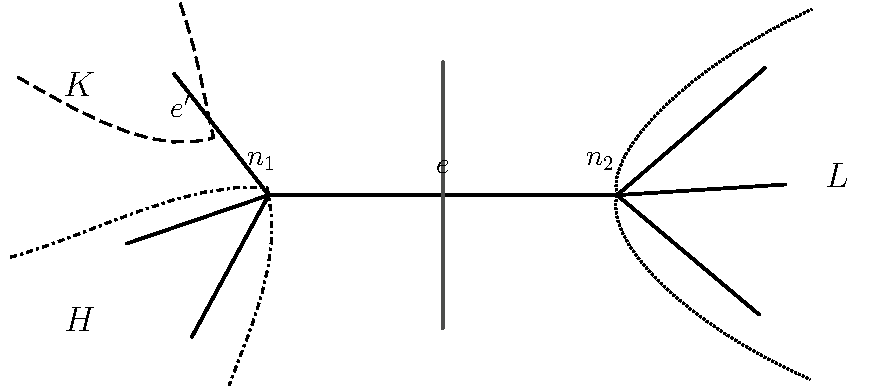
\includegraphics[width=0.72\textwidth]{bridge_three_block_symmetry_vector.pdf}
\caption{The three-block geometry of an ordered bridge chart
$\alpha=(e,e')$.  The principal edge $e$ and its adjacent selected edge $e'$
meet at $n_1$; $n_2$ is the other endpoint of $e$.  If $k$ is the endpoint
atom selected by $e'$, then
$K=C_k$, $H=C_{k^+\setminus\{k\}}$, and $L=C_{\bar k}$.  The long-dashed,
dash-dotted, and dotted curves delimit $K,H,L$, respectively.  The solid
transversal bar marks the split induced by $e$; neither it nor the block
boundaries are additional tree edges.  Reversal of the ordered pair
reindexes $(K,H,L)$ as $(L,H,K)$.}
\label{fig:three-block-bridge}
\end{figure}

\noindent
The geometry in Figure~\ref{fig:three-block-bridge} gives
\[
K^+=K\sqcup H,
\qquad
L^+=L\sqcup H,
\qquad
1-c_K=c_{L^+},
\qquad
1-c_L=c_{K^+}.
\]
Here and in the bridge-reversal lemma below, if $A\subseteq X$ is a taxon
block then
\[
c_A:=\frac{|A|}{N},\qquad
a_{i,A}:=\frac{|R_i\cap A|}{N}.
\]
Thus subscripts such as $K,L,K^+,L^+$ name taxon blocks, whereas lower-case
subscripts such as $k,\bar k,k^+$ name the corresponding atom index or
aggregate index block in a fixed chart.
These four block identities are the source of the coefficient correspondences
$(A.22)\leftrightarrow(A.23)$ and
$(A.24)\leftrightarrow(A.25)$.


The next lemma gives the coefficient-transfer mechanism used at every
bridge-reversal step.  It applies to the complete ordered-bridge sum, not to
a fixed chart in isolation.

\begin{lemma}[Bridge-reversal correspondence of the endpoint square faces]
\label{lem:bridge-ledger}
Let $\alpha=(e,e')$ be an ordered pair of adjacent relevant edges.  Removing
$e,e'$ gives three blocks $(K_\alpha,H_\alpha,L_\alpha)$, where $K_\alpha$
and $L_\alpha$ are the endpoint blocks and $H_\alpha$ is the middle block.
For the reversed chart $\rho\alpha=(e',e)$,
\[
(K_{\rho\alpha},H_{\rho\alpha},L_{\rho\alpha})
=(L_\alpha,H_\alpha,K_\alpha).
\]
\begin{samepage}
For every test function $Z:X\to\mathbb R$ satisfying
$\sum_{t\in X}Z(t)=0$, define, for every taxon block $A\subseteq X$,
\[
 x_{Z,A}:=\frac1N\sum_{t\in A}Z(t),
\]
and put
\[
 X_\alpha(Z):=x_{Z,L_\alpha},\qquad
 Y_\alpha(Z):=x_{Z,K_\alpha}.
\]
Then
\[
\Lambda_\alpha(Z)
=c_{K_\alpha}X_\alpha(Z)-c_{L_\alpha}Y_\alpha(Z)
\]
satisfies $\Lambda_{\rho\alpha}(Z)=-\Lambda_\alpha(Z)$.  When $Z$ is fixed,
write $X_\alpha:=X_\alpha(Z)$ and $Y_\alpha:=Y_\alpha(Z)$.
For the plus form, also fix all data in the other coordinate: a row principal
chart and a row relation $(i,j)$, with $\bar i$ and $\bar j$ denoting the
corresponding opposite row blocks.  These spectator data are held fixed when
$\alpha$ is replaced by $\rho\alpha$.  Put
\[
 X_\alpha^D(i):=x_{\bar i,L_\alpha}+x_{i,L_\alpha},\qquad
 Y_\alpha^D(i):=x_{\bar i,K_\alpha}+x_{i,K_\alpha},
\]
so that
\[
\Lambda_\alpha^D(i)
=c_{K_\alpha}X_\alpha^D(i)-c_{L_\alpha}Y_\alpha^D(i)
\]
satisfies the same reversal identity.  Moreover, define the two symmetric
coefficients
\[
r_s^\alpha=\frac12\left(\frac{a_{s,K_\alpha}}{c_{K_\alpha}}
+\frac{a_{s,L_\alpha}}{c_{L_\alpha}}\right),
\qquad s\in\{i,j\}.
\]
Both are invariant under reversal:
$r_i^{\rho\alpha}=r_i^\alpha$ and
$r_j^{\rho\alpha}=r_j^\alpha$.
\end{samepage}

Consequently, for either the ordinary pair $(X_\alpha,Y_\alpha)$ or the
$D$-row plus-form pair $(X_\alpha^D(i),Y_\alpha^D(i))$, reversal interchanges
the first and second endpoint square faces while preserving their symmetric
weights.  Since $\rho$ is a fixed-point-free involution of the full
ordered-adjacent summation range, the $X^2$ coefficients in one orientation
therefore give the $Y^2$ coefficients after global reindexing.  At the
ordinary-polynomial level, the map sends
the second endpoint square face
$c_{L_\alpha}^{2}r_i^\alpha r_j^\alpha Y_\alpha^2$ to
$c_{K_{\rho\alpha}}^{2}r_i^{\rho\alpha}
r_j^{\rho\alpha}X_{\rho\alpha}^2$.  This lemma asserts only that abstract
transport statement.  Its concrete application is carried out after the four
completion formulas have been introduced and expanded.
\end{lemma}

\begin{proof}
Reversing the ordered pair interchanges $K_\alpha$ and $L_\alpha$ and leaves
$H_\alpha$ fixed, so
both displayed contrasts change only by an overall sign.  The formula for
each $r_s^\alpha$, $s\in\{i,j\}$, is symmetric in
$K_\alpha,L_\alpha$, so both coefficients are reversal-invariant.  Also
$c_{K_{\rho\alpha}}=c_{L_\alpha}$ and
$X_{\rho\alpha}(Z)^2=Y_\alpha(Z)^2$, with the analogous identity for the plus
pair.  These identities prove the endpoint-square-face correspondence
directly.  No completion formula is used at this point.  The later
completion-coefficient table verifies the four concrete substitutions.
Finally
$\rho^2=\mathrm{id}$ and
$\rho\alpha\ne\alpha$, proving that reversal is a bijective reindexing of the
full ordered-chart range.
\end{proof}

In the forward chart, the notation of
Figure~\ref{fig:three-block-bridge} means
\[
(K,H,L)=\bigl(C_k,C_{k^+\setminus\{k\}},C_{\bar k}\bigr).
\]
In the reversed chart the selected, middle, and opposite taxon blocks are
$(L,H,K)$.  Hence
\[
1-c_K=c_H+c_L=c_{L^+},\qquad
1-c_L=c_H+c_K=c_{K^+}.
\]
If $k$ is the selected atom index in the forward chart and $k^\rho$ is the
selected atom index in the reversed chart, these equalities read
$1-c_k=c_{(k^\rho)^+}$ and $1-c_{k^\rho}=c_{k^+}$, with each aggregate taken
in its own chart.  They are cross-chart block identities, not a replacement
of an atom by an aggregate in one chart.
This is the block symmetry behind the coefficient pairs
\[
(A.22)\longleftrightarrow(A.23),\qquad
(A.24)\longleftrightarrow(A.25).
\]
Thus bridge reversal pairs the four square completions.

\subsection{Why bridge reversal is a global reindexing}\label{subsec:sym-red}

Every use of the column bridge reversal in this subsection means the
bijective change of summation index
$\alpha=(f,g)\mapsto\rho\alpha=(g,f)$ on the complete ordered-adjacent
range.  If a row principal edge $e$ and row indices $i,j$ are present, they
are held fixed, so the principal chart changes from $(e,f)$ to $(e,g)$.
The taxon-block triple changes from $(K_\alpha,H_\alpha,L_\alpha)$ to
$(L_\alpha,H_\alpha,K_\alpha)$.  Lemma~\ref{lem:bridge-ledger} therefore
identifies the second-square coefficient in the chart $(e,f)$ with the
first-square coefficient in the reversed chart $(e,g)$ and cancels the two
ordinary endpoint square faces only after summation over the full ordered
range.
No same-chart coefficient identity is asserted.  After this reindexing, the
remaining coefficients are calculated directly from the seven terms in
\eqref{eq:master-residual-numerator}; the row and column refinements are never
identified term by term.

\subsection{The available first-square coefficient: derivation of (A.21)}

Fix a principal chart $\chi$ and a row relation
$(i,j)\in I_{\rm r}^\chi$.  For every
$u\in\Omega_{\rm c}^\chi$ put
\[
X_u:=x_{\bar i,\bar u},
\]
and, only for an endpoint $k\in a_{\rm c}^\chi\cup b_{\rm c}^\chi$, put
\[
Y_k:=x_{\bar i,k}.
\]
The retained $I$-row component of the fixed-chart seven-source numerator
uses $2\mathcal R_1-\mathcal R_2$, not a single copy of
\eqref{eq:A17}.
Using
\[
(\Omega_{\rm c}^\chi)^2
=(I_{\rm c}^\chi\cup D_{\rm c}^\chi)
\sqcup\Delta_{a_{\rm c}^\chi}\sqcup\Delta_{b_{\rm c}^\chi},
\]
direct expansion gives the complete identity
\[
\begin{aligned}
&2\sum_{(u,l)\in(\Omega_{\rm c}^\chi)^2}
 r_i^uc_u r_j^lc_lX_u^2
-\sum_{k\in a_{\rm c}^\chi\cup b_{\rm c}^\chi}
 r_i^kr_j^k(c_kX_k-c_{\bar k}Y_k)^2\\
&\quad=
2\sum_{(u,l)\in I_{\rm c}^\chi\cup D_{\rm c}^\chi}
 r_i^uc_u r_j^lc_lX_u^2\\
&\qquad\quad+
\sum_{k\in a_{\rm c}^\chi\cup b_{\rm c}^\chi}
r_i^kr_j^k\bigl(
c_k^2X_k^2+2c_kc_{\bar k}X_kY_k-c_{\bar k}^2Y_k^2
\bigr).
\end{aligned}
\]
Thus the negative neighboring square removes one of the two positive
endpoint diagonals, changes the sign of its mixed term, and leaves a negative
second endpoint square face.  The formal chart-indexed notation and the
complete table of the three endpoint-indexed monomial faces are given in
\eqref{eq:direct-row-polynomial} and the table following it.  The
reversal-paired first and negative second endpoint square faces have not
disappeared chartwise; their cancellation over the full bridge orbit is
precisely \eqref{eq:direct-endpoint-face-cancellation}.

The magnitude of the first endpoint diagonal removed by
$-\mathcal R_2$ is
\begin{equation}\label{eq:A19}
\sum_{(i,j)\in I_{\rm r}}\sum_{k\in a_{\rm c}\cup b_{\rm c}}
r_i^kr_j^kc_k^2.
\tag{A.19}
\end{equation}
The corresponding mixed face enters with the positive sign
\begin{equation}\label{eq:A20}
2\sum_{(i,j)\in I_{\rm r}}\sum_{k\in a_{\rm c}\cup b_{\rm c}}
r_i^kr_j^kc_kc_{\bar k}X_kY_k.
\tag{A.20}
\end{equation}
After the endpoint square faces are paired over the complete bridge orbit, the
remaining polynomial has two copies of the nonendpoint first-square pool and
one copy of the mixed face.  One first-square copy together with the mixed
face forms the following first-square completion ledger:
Here and below, the superscript $\mathrm{rep}$ means
\emph{representative-square ledger}.
\begin{equation}\label{eq:A21}
\begin{aligned}
\mathcal C_I^{\mathrm{rep}}
:=
\sum_{(i,j)\in I_{\rm r}^\chi}\bigg[
&\sum_{(u,l)\in I_{\rm c}^\chi\cup D_{\rm c}^\chi}
 r_i^uc_u r_j^lc_l X_u^2\\
&+2\sum_{k\in a_{\rm c}^\chi\cup b_{\rm c}^\chi}
 r_i^kr_j^kc_kc_{\bar k}X_kY_k
\bigg].
\end{aligned}
\tag{A.21}
\end{equation}
Equation~\eqref{eq:A21} is therefore a first-square completion ledger: it
records both the available $X^2$ coefficient and the mixed $XY$ term that
must be absorbed.  It is neither a single square face nor the complete
fixed-chart polynomial $2\mathcal R_1-\mathcal R_2$.
Lemma~\ref{lem:bridge-ledger} supplies the matching second-square coefficient
by reindexing the complete global sum through the reversed chart.  It does
not replace $k$ by $\bar k$ within a fixed chart.

The $D$-row calculation is parallel and is recorded explicitly.  For
$(i,j)\in D_{\rm r}^\chi$, put
\[
X_u^D:=x_{\bar i,\bar u}+x_{i,\bar u},\qquad
Y_k^D:=x_{\bar i,k}+x_{i,k}.
\]
Its parallel first-square completion ledger is
\[
\begin{aligned}
\mathcal C_D^{\mathrm{rep}}
:=\sum_{(i,j)\in D_{\rm r}^\chi}\bigg[
&\sum_{(u,l)\in I_{\rm c}^\chi\cup D_{\rm c}^\chi}
r_i^uc_u r_j^lc_l(X_u^D)^2\\
&+2\sum_{k\in a_{\rm c}^\chi\cup b_{\rm c}^\chi}
r_i^kr_j^kc_kc_{\bar k}X_k^DY_k^D
\bigg].
\end{aligned}
\]
The complete table of its three endpoint-indexed monomial faces is obtained
from the displayed $I$-row table by the substitution
$(X_k,Y_k)\mapsto(X_k^D,Y_k^D)$.  Hence the ordinary and $D$-row plus-form
rows use
the same numerical coefficients but remain separate polynomial families.

\subsection{Completion of the cross term: equations (A.22)--(A.25)}

We now split the mixed coefficient in \eqref{eq:A21} among four completed
squares.
For $k\in a_{\rm c}^\chi\cup b_{\rm c}^\chi$,
\begin{equation}\label{eq:rikrjk}
 r_i^kr_j^kc_kc_{\bar k}
=\frac14\left(\frac{c_{\bar k}}{c_k}a_{i,k}a_{j,k}+a_{i,k}a_{j,\bar k}+a_{i,\bar k}a_{j,k}+\frac{c_k}{c_{\bar k}}a_{i,\bar k}a_{j,\bar k}\right).
\tag{A.21a}
\end{equation}
The selected endpoint block, its opposite block, and its same-side aggregate
are nonempty.  Hence
\[
c_k>0,\qquad c_{\bar k}>0,\qquad c_{k^+}>0,\qquad 1-c_k>0,
\]
so every denominator and square root in the next four displays is well
defined.
Thus the cross term in \eqref{eq:A21} is absorbed by the following four square sums:
\begin{equation}\label{eq:A22}
\frac14\sum_{(i,j)\in I_{\rm r}^\chi}
\sum_{k\in a_{\rm c}^\chi\cup b_{\rm c}^\chi}
 c_k\frac{a_{i,\bar k}a_{j,\bar k}}{c_{\bar k}}
\left(\sqrt{\frac{1-c_k}{c_{\bar k}}}x_{\bar i,\bar k}+\sqrt{\frac{c_{\bar k}}{1-c_k}}x_{\bar i,k}\right)^2,
\tag{A.22}
\end{equation}
\begin{equation}\label{eq:A23}
\frac14\sum_{(i,j)\in I_{\rm r}^\chi}
\sum_{k\in a_{\rm c}^\chi\cup b_{\rm c}^\chi}
 c_{\bar k}\frac{a_{i,k}a_{j,k}}{c_k}
\left(\sqrt{\frac{c_k}{c_{k^+}}}x_{\bar i,\bar k}+\sqrt{\frac{c_{k^+}}{c_k}}x_{\bar i,k}\right)^2,
\tag{A.23}
\end{equation}
\begin{equation}\label{eq:A24}
\frac14\sum_{(i,j)\in I_{\rm r}^\chi}
\sum_{k\in a_{\rm c}^\chi\cup b_{\rm c}^\chi}
 a_{i,k}a_{j,\bar k}(x_{\bar i,\bar k}+x_{\bar i,k})^2,
\tag{A.24}
\end{equation}
\begin{equation}\label{eq:A25}
\frac14\sum_{(i,j)\in I_{\rm r}^\chi}
\sum_{k\in a_{\rm c}^\chi\cup b_{\rm c}^\chi}
 a_{i,\bar k}a_{j,k}(x_{\bar i,\bar k}+x_{\bar i,k})^2.
\tag{A.25}
\end{equation}
The numerical coefficients are justified by the following elementary
identities.  For any scalar $\gamma$ and formal variables $X,Y$,
\[
\frac14\gamma(X+Y)^2
=\frac14\gamma X^2+\frac12\gamma XY+\frac14\gamma Y^2.
\]
More generally, for any positive scalar $s$,
\[
\frac14\gamma(sX+s^{-1}Y)^2
=
\frac14\gamma s^2X^2+\frac12\gamma XY
+\frac14\gamma s^{-2}Y^2.
\]
Fix the chart $\chi$ and one triple $(i,j,k)$, and in the corresponding
summand of (A.22)--(A.25) write
$X:=x_{\bar i,\bar k}$ and $Y:=x_{\bar i,k}$.  For any polynomial
$F(X,Y)$ and monomial $M$, write
$[M]F:=\operatorname{coeff}_M(F)$.  For
\[
t\in\{22,23,24,25\},
\qquad
M\in\{X^2,XY,Y^2\},
\]
define
\[
[M]_t
:=
\operatorname{coeff}_{M}
\left(
\text{the fixed $(i,j,k)$-summand of equation (A.$t$)}
\right).
\]
Thus the subscript $t$ names the source equation, while the expression
inside the brackets names the monomial whose coefficient is extracted.  The
dependence on $\chi,i,j,k$ is suppressed only to keep the table readable.
For example, the outside coefficient and the square of the $X$-multiplier in
(A.22) give
\[
[X^2]_{22}
=
\left(\frac14c_k\frac{a_{i,\bar k}a_{j,\bar k}}{c_{\bar k}}\right)
\left(\frac{1-c_k}{c_{\bar k}}\right)
=
\frac14\frac{c_k(1-c_k)}{c_{\bar k}^2}
a_{i,\bar k}a_{j,\bar k}.
\]
Direct expansion gives all twelve coefficients:
\[
\begin{aligned}
[X^2]_{22}
&=\frac14\frac{c_k(1-c_k)}{c_{\bar k}^2}
  a_{i,\bar k}a_{j,\bar k},&
[XY]_{22}
&=\frac12\frac{c_k}{c_{\bar k}}
  a_{i,\bar k}a_{j,\bar k},\\
[Y^2]_{22}
&=\frac14\frac{c_k}{1-c_k}
  a_{i,\bar k}a_{j,\bar k},\\[1mm]
[X^2]_{23}
&=\frac14\frac{c_{\bar k}}{c_{k^+}}a_{i,k}a_{j,k},&
[XY]_{23}
&=\frac12\frac{c_{\bar k}}{c_k}a_{i,k}a_{j,k},\\
[Y^2]_{23}
&=\frac14\frac{c_{\bar k}c_{k^+}}{c_k^2}a_{i,k}a_{j,k},\\[1mm]
[X^2]_{24}&=\frac14a_{i,k}a_{j,\bar k},&
[XY]_{24}&=\frac12a_{i,k}a_{j,\bar k},&
[Y^2]_{24}&=\frac14a_{i,k}a_{j,\bar k},\\
[X^2]_{25}&=\frac14a_{i,\bar k}a_{j,k},&
[XY]_{25}&=\frac12a_{i,\bar k}a_{j,k},&
[Y^2]_{25}&=\frac14a_{i,\bar k}a_{j,k}.
\end{aligned}
\]
Define the chart-indexed first- and second-square coefficients by
\[
p_{ij}^{\chi}(k):=\sum_{t=22}^{25}[X^2]_t,
\qquad
q_{ij}^{\chi}(k):=\sum_{t=22}^{25}[Y^2]_t.
\]
When the chart is fixed, we suppress the superscript $\chi$ and write
$p_{ij}(k),q_{ij}(k)$.
Adding the four mixed coefficients and using \eqref{eq:rikrjk} gives
\[
\sum_{t=22}^{25}[XY]_{t}
=2c_kc_{\bar k}r_i^kr_j^k,
\]
which is exactly the coefficient in \eqref{eq:A20}.

The total first- and second-square coefficients consumed by the completed
package are therefore
\[
\begin{aligned}
4p_{ij}(k)
={}&
\frac{c_k(1-c_k)}{c_{\bar k}^2}a_{i,\bar k}a_{j,\bar k}
+\frac{c_{\bar k}}{c_{k^+}}a_{i,k}a_{j,k}\\
&+a_{i,k}a_{j,\bar k}+a_{i,\bar k}a_{j,k},\\
4q_{ij}(k)
={}&
\frac{c_k}{1-c_k}a_{i,\bar k}a_{j,\bar k}
+\frac{c_{\bar k}c_{k^+}}{c_k^2}a_{i,k}a_{j,k}\\
&+a_{i,k}a_{j,\bar k}+a_{i,\bar k}a_{j,k}.
\end{aligned}
\]
Finally, let $\alpha$ have three-block data $(K,H,L)$ and let
$\rho\alpha$ have $(L,H,K)$.  Since
$1-c_K=c_{L^+}$ and $1-c_L=c_{K^+}$, the preceding twelve coefficients
give the four coefficient-preserving identities below.  In this display,
$[M](\mathrm{A.}t)_\alpha$ means the coefficient of $M$ in the fixed
$(i,j,k)$-summand of equation (A.$t$) belonging to the ordered bridge
$\alpha$:
\[
\begin{aligned}
[Y^2](A.22)_\alpha&=[X^2](A.23)_{\rho\alpha},&
[Y^2](A.23)_\alpha&=[X^2](A.22)_{\rho\alpha},\\
[Y^2](A.24)_\alpha&=[X^2](A.25)_{\rho\alpha},&
[Y^2](A.25)_\alpha&=[X^2](A.24)_{\rho\alpha}.
\end{aligned}
\]
This is the explicit coefficient calculation behind
$(A.22)\leftrightarrow(A.23)$ and
$(A.24)\leftrightarrow(A.25)$; no same-chart substitution is used.

\subsection{Expansion of the available square coefficient: equations (A.26)--(A.29)}

It remains to express the available first-square coefficient in the common
$a$-monomial language used in the final collection.
The two factors in the square coefficient satisfy
\[
2c_kr_i^k=a_{i,k}+\frac{c_k}{c_{\bar k}}a_{i,\bar k},
\qquad
2c_lr_j^l=a_{j,l}+\frac{c_l}{c_{\bar l}}a_{j,\bar l}.
\]
Multiplying these two binomials, without suppressing any term, gives
\begin{equation}\label{eq:A26to29}
\begin{aligned}
4r_i^kc_k r_j^lc_l
&=\left(a_{i,k}+\frac{c_k}{c_{\bar k}}a_{i,\bar k}\right)
  \left(a_{j,l}+\frac{c_l}{c_{\bar l}}a_{j,\bar l}\right)\\
&=a_{i,k}a_{j,l}
+\frac{c_l}{c_{\bar l}}a_{i,k}a_{j,\bar l}
+\frac{c_k}{c_{\bar k}}a_{i,\bar k}a_{j,l}
+\frac{c_kc_l}{c_{\bar k}c_{\bar l}}a_{i,\bar k}a_{j,\bar l}.
\end{aligned}
\tag{A.26--A.29}
\end{equation}
The four summands reproduce, in order, the original equations (26), (27),
(28), and (29).  In particular, the denominator $c_{\bar l}$ belongs to the
term containing $a_{j,\bar l}$, whereas $c_{\bar k}$ belongs to the term
containing $a_{i,\bar k}$.


\subsection{From the four determinant levels to four square families}

We now assemble the preceding local identities.  All equalities are
equalities of quadratic polynomials.  The order is important: first expand
the four determinant levels into seven terms, then decompose the row
coordinate for each fixed column term, next pair the endpoint square faces by
bridge reversal, and finally sum the remaining coefficient over each
same-side column block.  The row and column refinements remain distinct
throughout.

\paragraph{Dependency map for Subsections A.4--A.7.}
The preliminary expansion below obtains the seven-source numerator from the
determinant-level identities of Subsection~A.3.  Step~1 in the proof of
Lemma~\ref{lem:master-coefficient-ledger} then decomposes the row coordinate
while keeping each column term fixed.  Once the retained row polynomial has
been isolated, Subsections~A.4--A.7 enter in the following precise way:
\begin{center}
\small
\renewcommand{\arraystretch}{1.25}
\begin{tabular}{@{}
>{\raggedright\arraybackslash}p{0.10\textwidth}
>{\raggedright\arraybackslash}p{0.36\textwidth}
>{\raggedright\arraybackslash}p{0.43\textwidth}
@{}}
\toprule
\text{input}&\text{object supplied to A.8}&\text{exact use inside A.8}\\
\midrule
A.4&
the global bridge-reversal reindexing, with first and second square faces
interchanged only in the reversed chart&
equation (A.29e) cancels the ordinary endpoint square faces, and the
$q$-to-$p$ reindexing in (A.29f) transfers the second square face of a
completed package to the first square face in the reversed chart\\
A.5&
the available first-square pool and the three endpoint-indexed monomial
faces: first square, mixed, and negative second square&
these terms are named and collected in (A.29d); they become the available
coefficient and the contributions $d_kZ^2$, $m_kZW$, and $-e_kW^2$ in
Step~2\\
A.6&
the four completed squares (A.22)--(A.25), together with their first,
mixed, and second monomial coefficients&
their sum is the completed-square package used in (A.29f); its mixed
coefficient absorbs the retained cross term, while its two square
coefficients record the amounts consumed on the first and second square
faces\\
A.7&
the four-term expansion (A.26)--(A.29) of the available square coefficient
in the common $a$-monomial language&
Step~3 compares that expansion with the completed-package coefficient and
the six rows of the remaining coefficient, producing the block identity
(A.30b) and then (A.29g)\\
\bottomrule
\end{tabular}
\end{center}
Thus A.8 is not a second independent local calculation.  It first uses A.5
to supply the uncompleted coefficient ledger, uses A.4 twice to settle the
reversal-paired endpoint square faces globally, uses A.6 to complete the
mixed term, and uses A.7 to identify the coefficient left after that
completion.  In terms of the
stable equation labels, the three remaining assembly steps are
\[
\begin{aligned}
\text{Step 2:}\quad&
\text{(A.21)}
\longrightarrow\text{(A.29d)}
\longrightarrow\text{(A.29e)}
\longrightarrow\text{(A.29f)},\\
\text{Step 3:}\quad&
\text{(A.29f)}
\longrightarrow\text{(A.30b)}
\longrightarrow\text{(A.29g)},\\
\text{Step 4:}\quad&
\text{(A.29g)}
\longrightarrow\text{(A.29h)}.
\end{aligned}
\]
Step~1 performs the fixed-column row decomposition and cancels its boundary
over the complete row-bridge range.  Step~2 computes the retained row
polynomial, cancels its ordinary endpoint square faces, and inserts the
completed-square package.  Step~3 identifies the coefficient left after that
completion by summing one same-side block.  Step~4 restores the two row
multiplicities and identifies the four resulting terms with the four
nonnegative square families.

We first record the seven-source numerator used in Step~1.
Using the formally defined row--column transpose of (A.15a), the exact
seven-source identity is
\begin{equation}\label{eq:master-residual-numerator}
\begin{aligned}
4U-2R-2C+B
={}&U+2\mathcal R_1+\widetilde{\mathcal R}_1-\mathcal R_2\\
&-2\mathcal Q_1-\widetilde{\mathcal Q}_1+\mathcal Q_2.
\end{aligned}
\tag{A.29a}
\end{equation}
Indeed,
\[
U-R=\mathcal R_1-\mathcal Q_1,
\qquad
U-C=\widetilde{\mathcal R}_1-\widetilde{\mathcal Q}_1,
\qquad
C-B=\mathcal R_2-\mathcal Q_2.
\]
Equivalently,
\[
R=U-\mathcal R_1+\mathcal Q_1,\qquad
C=U-\widetilde{\mathcal R}_1+\widetilde{\mathcal Q}_1,\qquad
B=C-\mathcal R_2+\mathcal Q_2.
\]
Therefore
\[
\begin{aligned}
4U-2R-2C+B
&=4U-2(U-\mathcal R_1+\mathcal Q_1)-C-\mathcal R_2+\mathcal Q_2\\
&=2U+2\mathcal R_1-2\mathcal Q_1
 -(U-\widetilde{\mathcal R}_1+\widetilde{\mathcal Q}_1)
 -\mathcal R_2+\mathcal Q_2\\
&=U+2\mathcal R_1+\widetilde{\mathcal R}_1-\mathcal R_2
 -2\mathcal Q_1-\widetilde{\mathcal Q}_1+\mathcal Q_2,
\end{aligned}
\]
which proves every sign and multiplicity in \eqref{eq:master-residual-numerator}.

\paragraph{Why the row and column refinements remain distinct.}
Fix a principal chart $\chi$.  For a row atom $i$ and a column atom $u$, put
\[
 \alpha_{i,u}^{\chi}:=c_ur_i^u
 =\frac12\left(a_{i,u}+\frac{c_u}{c_{\bar u}}a_{i,\bar u}\right).
\]
For the transposed first passage, the preceding definition gives
\[
 \beta_{i,u}^{\chi}:=r_i\check r_u^i
 =\frac12\left(a_{i,u}+\frac{r_i}{r_{\bar i}}a_{\bar i,u}\right).
\]
The two refinements need not agree.  Their difference is
\[
 \alpha_{i,u}^{\chi}-\beta_{i,u}^{\chi}
 =\frac12\left(
 \frac{c_u}{c_{\bar u}}a_{i,\bar u}
 -\frac{r_i}{r_{\bar i}}a_{\bar i,u}
 \right).
\]
This difference is not identically zero as a function of the chart data,
although it may vanish for particular choices of $\chi,i,u$.
Since
$\nu_u=\sum_{i\in\Omega_{\rm r}^\chi}\beta_{i,u}^{\chi}$, the two products
\[
 \omega_i\omega_j
 =\sum_{u,l\in\Omega_{\rm c}^\chi}
   \alpha_{i,u}^{\chi}\alpha_{j,l}^{\chi},
 \qquad
 \nu_u\nu_l
 =\sum_{i,j\in\Omega_{\rm r}^\chi}
   \beta_{i,u}^{\chi}\beta_{j,l}^{\chi}
\]
retain the different ordered index pairs $(i,u),(j,l)$ and are not equated
term by term.
Both $\alpha_{i,u}^{\chi}$ and $\beta_{i,u}^{\chi}$ are chart-local
quantities.  Their superscript is suppressed only inside one fixed-chart
calculation.  Whenever
they occur inside a sum over $\chi$, their masses, opposite blocks, and
aggregates are evaluated in that summand's chart $\chi$.  These subscripted
scalar weights are unrelated to the bare symbol $\alpha$ used for an ordered
bridge.

We therefore regroup the seven terms before applying either refinement:
\begin{equation}\label{eq:direct-seven-source-regrouping}
\begin{aligned}
4U-2R-2C+B
&=2[U+\mathcal R_1-\mathcal Q_1]\\
&\quad-[U-\widetilde{\mathcal R}_1+
 \widetilde{\mathcal Q}_1+\mathcal R_2-\mathcal Q_2]\\
&=2(2U-R)-(2C-B).
\end{aligned}
\tag{A.29b}
\end{equation}
The following table verifies the coefficient of each of the seven terms:
\[
\begin{array}{c|rrrrrrr}
\toprule
&U&\mathcal R_1&\widetilde{\mathcal R}_1&\mathcal R_2
&\mathcal Q_1&\widetilde{\mathcal Q}_1&\mathcal Q_2\\
\midrule
2[U+\mathcal R_1-\mathcal Q_1]&2&2&0&0&-2&0&0\\
-[U-\widetilde{\mathcal R}_1+\widetilde{\mathcal Q}_1
 +\mathcal R_2-\mathcal Q_2]&-1&0&1&-1&0&-1&1\\
\midrule
\text{total}&1&2&1&-1&-2&-1&1\\
\bottomrule
\end{array}
\]
The coefficient table shows directly that the transposed bracket reconstructs
$C$ before the row residual identity is applied.  This is the reason no
termwise equality between $\alpha_{i,u}^{\chi}$ and
$\beta_{i,u}^{\chi}$ is needed.

For $k\in a^\chi\cup b^\chi$, both $k$ and its opposite block $\bar k$
are nonempty.  Hence
\[
c_k>0,\qquad c_{\bar k}>0,\qquad c_{k^+}\ge c_k>0,
\qquad
1-c_k=c_{\bar k}+c_{k^+\setminus\{k\}}>0.
\]
All denominators and square roots below are therefore well defined.  For
independent formal variables $X,Y$, define the completed-square polynomial
\begin{equation}\label{eq:P-package}
\begin{aligned}
\mathcal P_{ij,k}(X,Y):={}&\frac14c_k
 \frac{a_{i,\bar k}a_{j,\bar k}}{c_{\bar k}}
 \left(\sqrt{\frac{1-c_k}{c_{\bar k}}}X
      +\sqrt{\frac{c_{\bar k}}{1-c_k}}Y\right)^2\\
&+\frac14c_{\bar k}\frac{a_{i,k}a_{j,k}}{c_k}
 \left(\sqrt{\frac{c_k}{c_{k^+}}}X
      +\sqrt{\frac{c_{k^+}}{c_k}}Y\right)^2\\
&+\frac14a_{i,k}a_{j,\bar k}(X+Y)^2
 +\frac14a_{i,\bar k}a_{j,k}(X+Y)^2.
\end{aligned}
\end{equation}
When more than one principal chart is present, we write
$\mathcal P_{ij,k}^{\chi}$ for the polynomial whose masses and aggregates are
computed in chart $\chi$; within one fixed chart the superscript is suppressed.
Also define
\begin{equation}\label{eq:Psi-exact}
\begin{aligned}
\Psi_{ij}^{\chi}(u):={}&
\sum_{l\in M_{S,\chi}(u)}
 \frac{c_{\bar u}}{c_{u^+}}a_{i,u}a_{j,l}
+\sum_{l\in S_\chi(u)}4c_uc_l r_i^{u,\chi}r_j^{l,\chi}\\
&+\mathbf1_{u\in c^\chi\cup d^\chi}
 \bigl(a_{i,u}a_{j,\bar u}+a_{i,\bar u}a_{j,u}\bigr)\\
&-\sum_{l\in M_{S,\chi}(u)}
 \frac{c_uc_l}{c_{\bar u}c_{\bar l}}
 a_{i,\bar u}a_{j,\bar l}
-\mathbf1_{u\in a^\chi\cup b^\chi}
 4c_u^2r_i^{u,\chi}r_j^{u,\chi}\\
&+\sum_{l\in M_{D,\chi}(u)}
 \left(
 \frac{c_u}{c_{\bar u}}a_{i,\bar u}a_{j,l}
 +\frac{c_l}{c_{\bar l}}a_{i,u}a_{j,\bar l}
 \right).
\end{aligned}
\tag{A.30a}
\end{equation}

For reference, the six rows of \eqref{eq:Psi-exact} are organized as follows;
the terms themselves are exactly those displayed in that equation.
\begin{table}[ht]
\centering
\small
\begin{tabular}{ccl}
\toprule
\text{row}&\text{support or index set}&\text{role in the coefficient}\\
\midrule
1&$l\in M_{S,\chi}(u)$&same-side endpoint contribution\\
2&$l\in S_\chi(u)$&same-side symmetric contribution\\
3&$u\in c^\chi\cup d^\chi$&nonendpoint residual contribution\\
4&$l\in M_{S,\chi}(u)$&same-side subtraction\\
5&$u\in a^\chi\cup b^\chi$&endpoint diagonal subtraction\\
6&$l\in M_{D,\chi}(u)$&opposite-side residual contribution\\
\bottomrule
\end{tabular}
\caption{The six terms of $\Psi_{ij}^\chi(u)$ in \eqref{eq:Psi-exact}.}
\label{tab:Psi-six-rows}
\end{table}

\begin{lemma}[Row decomposition with one column term fixed]
\label{lem:occurrence-row-settlement}
Fix a column principal edge $f\in E_2(T_2^\circ)$.  The column term $\eta$
is either the ordinary split $\eta=\tau_f$ or one adjacent side-pair
$\eta=C_{f,h}$ for one ordered adjacent pair
$(f,h)\in\overrightarrow A_2(T_2^\circ)$.  In the second case let
$k=k(f,h)\in a_f\cup b_f$ be the endpoint atom of $\Pi_f$ indexed by $h$.

Now fix a row principal edge $e\in E_2(T_1^\circ)$ and work in the
principal chart $\chi=(e,f)$.  Choose either side of the split $\tau_f$ and
let $B_f\subseteq\Omega_f^{\rm c}$ be the set of column atom indices whose
taxon union is that side.  Put
\[
 S_f:=\Omega_f^{\rm c}\setminus B_f.
\]
Thus $C_{B_f}$ and $C_{S_f}$ are the two taxon sides of $\tau_f$.  For
an actual row taxon block $A\subseteq X$, define
\[
a_{A,p}:=\frac{|A\cap C_p|}{N},
\qquad
r_A^p:=\frac12\left(
\frac{a_{A,p}}{c_p}+\frac{a_{A,\bar p}}{c_{\bar p}}
\right),
\]
and define the row-chart-independent additive weight of $A$ for the fixed
column term $\eta$ by
\[
w^\eta(A):=
\begin{cases}
\displaystyle\sum_{p\in\Omega_f^{\rm c}}c_pr_A^p,
  &\eta=\tau_f,\\[2mm]
r_A^k,&\eta=C_{f,h}.
\end{cases}
\]
The masses and opposite blocks in this formula belong to the fixed column
chart of $f$.  Thus $w^\eta(A)$ depends on $A$ and the fixed column term
$\eta$, but not on the row principal edge used to partition $A$; moreover it
is additive on disjoint taxon blocks.  For $i\in\Omega_e^{\rm r}$ set
$w_i^\eta:=w^\eta(R_i)$ and define the two row forms by
\[
\begin{array}{c|c|c|c}
\toprule
\eta&w_i^\eta&X_i^\eta&Y_i^\eta\\
\midrule
\tau_f&
\displaystyle\sum_{p\in\Omega_f^{\rm c}}c_pr_i^p&
x_{\bar i,B_f}&x_{i,B_f}\\[1mm]
C_{f,h}&r_i^k&
c_kx_{\bar i,\bar k}-c_{\bar k}x_{\bar i,k}&
c_kx_{i,\bar k}-c_{\bar k}x_{i,k}\\
\bottomrule
\end{array}
\]
Put
\[
 w_{\bar i}^\eta:=w^\eta(R_{\bar i})
 =\sum_{j\in\bar i}w_j^\eta,
 \qquad
 \mathcal E_e:=a_e\cup b_e,
\]
and define the row-copy relation sets explicitly by
\[
 D_e:=\{(i,j)\in(\Omega_e^{\rm r})^2:
             i\in\mathcal E_e,\ j\in\bar i\},
 \qquad
 \Delta_{\mathcal E_e}:=\{(i,i):i\in\mathcal E_e\},
\]
\[
 I_e:=(\Omega_e^{\rm r})^2
       \setminus\bigl(D_e\sqcup\Delta_{\mathcal E_e}\bigr).
\]
All quantities below depend on this fixed choice of $\eta$:
\begin{align*}
E_e^\eta&:=T[\sigma_e,\eta]=(X_i^\eta)^2
 \quad\text{for any }i\in\Omega_e^{\rm r},\\
N_e^\eta&:=\sum_{\substack{g:\,(e,g)\in
 \overrightarrow A_2(T_1^\circ)}}T[C_{e,g},\eta]
 =\sum_{s\in\mathcal E_e}
 \bigl(w_s^\eta X_s^\eta-w_{\bar s}^\eta Y_s^\eta\bigr)^2,\\
I_e^\eta&:=\sum_{(i,j)\in I_e}
 w_i^\eta w_j^\eta(X_i^\eta)^2,\\
D_e^\eta&:=\sum_{(i,j)\in D_e}
 w_i^\eta w_j^\eta(X_i^\eta+Y_i^\eta)^2,\\
\mathcal B_e^\eta&:=\sum_{s\in\mathcal E_e}
 (w_s^\eta+w_{\bar s}^\eta)
 \left(w_s^\eta(X_s^\eta)^2
       -w_{\bar s}^\eta(Y_s^\eta)^2\right).
\end{align*}
We call the explicitly displayed polynomial $\mathcal B_e^\eta$ the
\emph{row-boundary polynomial}.  Every later reference to the row boundary
means this polynomial, with the indicated $e$ and fixed column term $\eta$.
Then, for every $e$ and every fixed $\eta$,
\begin{equation}\label{eq:occurrence-row-settlement}
 2E_e^\eta-N_e^\eta
 =2I_e^\eta+D_e^\eta+\mathcal B_e^\eta.
\tag{A.29c$_0$}
\end{equation}
Moreover, the row boundary vanishes only after summing over the full range of row
principal edges:
\begin{equation}\label{eq:fixed-occurrence-boundary-cancellation}
 \sum_{e\in E_2(T_1^\circ)}\mathcal B_e^\eta=0
 \qquad\text{for every fixed }\eta.
\tag{A.29c$_1$}
\end{equation}

Finally, writing $U_{e,f},R_{e,f},C_{e,f},B_{e,f}$ for the four
polynomials of the principal chart $(e,f)$, the identification is
\[
\begin{array}{c|c|c}
\toprule
\eta&E_e^\eta&N_e^\eta\\
\midrule
\tau_f&U_{e,f}&R_{e,f}\\
C_{f,h}&T[\sigma_e,C_{f,h}]&
\displaystyle\sum_{\substack{g:\,(e,g)\in
\overrightarrow A_2(T_1^\circ)}}T[C_{e,g},C_{f,h}]\\
\bottomrule
\end{array}
\]
and hence, for every fixed $(e,f)$,
\begin{equation}\label{eq:occurrence-URCB-decomposition}
\begin{aligned}
E_e^{\tau_f}&=U_{e,f},&
N_e^{\tau_f}&=R_{e,f},\\
\sum_{\substack{h:\,(f,h)\in\overrightarrow A_2(T_2^\circ)}}
 E_e^{C_{f,h}}&=C_{e,f},&
\sum_{\substack{h:\,(f,h)\in\overrightarrow A_2(T_2^\circ)}}
 N_e^{C_{f,h}}&=B_{e,f}.
\end{aligned}
\tag{A.29c$_2$}
\end{equation}
Thus every indexed term in $U,R,C,B$ appears exactly once in these two
ranges.
\end{lemma}

\begin{proof}
For $\eta=\tau_f$, apply
Proposition~\ref{prop:weighted-centered-cancellation} to the central-side
partition $\Omega_f^{\rm c}=S_f\sqcup B_f$.  It identifies the summand
belonging to the endpoint atom $s=s(e,g)$ with
\[
 T[C_{e,g},\tau_f]
 =\bigl(w_s^{\tau_f}X_s^{\tau_f}
       -w_{\bar s}^{\tau_f}Y_s^{\tau_f}\bigr)^2.
\]
For $\eta=C_{f,h}$ the corresponding identity is the fixed-$k$ identity in
the proof of (A.15b):
\[
 T[C_{e,g},C_{f,h}]
 =\bigl(r_s^kX_s^{C_{f,h}}
       -r_{\bar s}^{\,k}Y_s^{C_{f,h}}\bigr)^2.
\]
The bijection $g\leftrightarrow s(e,g)$ from the formal chart construction
therefore proves the displayed formula for $N_e^\eta$ in both cases.
Changing the row orientation changes $X_i^\eta$ only by sign, so
$(X_i^\eta)^2=E_e^\eta$ for every $i$.

Both weight systems are nonnegative and additive on actual row blocks.
Their atomic normalizations are
\[
 \sum_{i\in\Omega_e^{\rm r}}w_i^{\tau_f}
 =\sum_{p\in\Omega_f^{\rm c}}c_p
   \sum_{i\in\Omega_e^{\rm r}}r_i^p=1,
 \qquad
 \sum_{i\in\Omega_e^{\rm r}}w_i^{C_{f,h}}
 =\sum_{i\in\Omega_e^{\rm r}}r_i^k=1.
\]
Lemma~\ref{lem:source-index-residual-passages} applies and gives
$E_e^\eta-N_e^\eta=I_e^\eta+D_e^\eta-Q_e^\eta$, where
\[
 Q_e^\eta=\sum_{s\in\mathcal E_e}
 w_{\bar s}^\eta(w_s^\eta+w_{\bar s}^\eta)(Y_s^\eta)^2.
\]
The disjoint partition
$(\Omega_e^{\rm r})^2=I_e\sqcup D_e\sqcup\Delta_{\mathcal E_e}$
also gives
\[
E_e^\eta-I_e^\eta
=\sum_{s\in\mathcal E_e}
 (w_s^\eta+w_{\bar s}^\eta)w_s^\eta(X_s^\eta)^2.
\]
The required identity is now obtained without suppressing the intermediate
coefficient:
\[
\begin{aligned}
2E_e^\eta-N_e^\eta
&=(E_e^\eta-N_e^\eta)+E_e^\eta\\
&=(I_e^\eta+D_e^\eta-Q_e^\eta)
  +I_e^\eta+(E_e^\eta-I_e^\eta)\\
&=2I_e^\eta+D_e^\eta
  +(E_e^\eta-I_e^\eta-Q_e^\eta)\\
&=2I_e^\eta+D_e^\eta+\mathcal B_e^\eta.
\end{aligned}
\]
This proves \eqref{eq:occurrence-row-settlement} and also shows exactly where
the row-boundary polynomial enters.

The row reversal used in the boundary sum is the explicit map
\[
\rho_{\rm r}:((e,g),\eta)\longmapsto((g,e),\eta);
\]
in particular, the column term $\eta$ remains fixed.  Now fix one
ordered row bridge
$\alpha=(e,g)$ with taxon blocks $(K_\alpha,H_\alpha,L_\alpha)$.
Let $s=s(e,g)$ be its endpoint atom in the chart of $e$, and define
\[
 X_\alpha^\eta:=X_s^\eta,
 \qquad
 Y_\alpha^\eta:=Y_s^\eta.
\]
Using additivity on row blocks, set
\[
 w_{K_\alpha}^\eta:=w_s^\eta,
 \qquad
 w_{L_\alpha}^\eta:=w_{\bar s}^\eta.
\]
Its endpoint summand in $\mathcal B_e^\eta$ is
\[
 (w_{K_\alpha}^\eta+w_{L_\alpha}^\eta)
 \left(w_{K_\alpha}^\eta (X_\alpha^\eta)^2
       -w_{L_\alpha}^\eta (Y_\alpha^\eta)^2\right).
\]
The reversed bridge $\rho_{\rm r}\alpha=(g,e)$ has endpoint/opposite blocks
$(L_\alpha,K_\alpha)$.  Additivity on row blocks and the fact that the fixed
column term $\eta$ is unchanged give
\[
 w_{K_{\rho_{\rm r}\alpha}}^\eta=w_{L_\alpha}^\eta,\qquad
 w_{L_{\rho_{\rm r}\alpha}}^\eta=w_{K_\alpha}^\eta,\qquad
 (X_{\rho_{\rm r}\alpha}^\eta)^2=(Y_\alpha^\eta)^2,\qquad
 (Y_{\rho_{\rm r}\alpha}^\eta)^2=(X_\alpha^\eta)^2.
\]
The reversed summand is therefore the negative of the forward summand.
Reversal is a fixed-point-free involution on
$\overrightarrow A_2(T_1^\circ)$, proving
\eqref{eq:fixed-occurrence-boundary-cancellation}.

The first row of the identification table is the definition of
$T[\sigma_e^+,\tau_f]$.  After summing the second row over all
$(f,h)\in\overrightarrow A_2(T_2^\circ)$, its $E_e^\eta$-entry and
$N_e^\eta$-entry are, respectively, the definitions of
$T[\sigma_e,\tau_f^+]$ and
$T[\sigma_e^+,\tau_f^+]$.  This proves
\eqref{eq:occurrence-URCB-decomposition} and the claim that each indexed term
appears once.
\end{proof}

\paragraph{Calligraphic-to-occurrence crosswalk.}
Fix the chart $\chi=(e,f)$ and put
\[
 H_f:=\{h\in E_2(T_2^\circ):
              (f,h)\in\overrightarrow A_2(T_2^\circ)\}.
\]
Thus $H_f$ consists of all relevant edges adjacent to $f$, with $f$ first in
the ordered pair.  For $h\in H_f$, let $k(f,h)\in a_f\cup b_f$ index the
endpoint atom $A_f(h)$ of $\Pi_f$.  In the column copy of the chart,
\[
 C_{k(f,h)}^\chi=A_f(h).
\]
This atom is not the whole adjacent side-pair correction $C_{f,h}$: if
$k=k(f,h)$, then
\[
 C_{f,h}=(K_{f,h},L_{f,h})
         =\bigl(C_k^\chi,C_{\bar k_\chi}^\chi\bigr).
\]

The map $h\mapsto k(f,h)$ from $H_f$ to $a_f\cup b_f$ is bijective.
For injectivity, let $h_1\ne h_2$.  If they meet the same endpoint of $f$,
then $A_f(h_1)$ and $A_f(h_2)$ lie in two distinct branches at that
endpoint; if they meet opposite endpoints, the two atoms lie in different
components of $T_2^\circ-f$.  In either case the atoms are nonempty and
disjoint, so $k(f,h_1)\ne k(f,h_2)$.  For surjectivity, recall that
$a_f\cup b_f$ is defined to index precisely the atoms $A_f(h)$ arising from
relevant edges $h$ adjacent to $f$.  Hence, for every endpoint-indexed
family $F(k)$,
\[
 \sum_{h\in H_f}F\bigl(k(f,h)\bigr)
 =\sum_{k\in a_f\cup b_f}F(k).
\]
Thus each ordered correction $C_{f,h}$ is in one-to-one correspondence with
one endpoint atom of $\Pi_f$ and is counted once.  This ``multiplicity one''
does not concern its polynomial coefficient; residual indices in
$c_f\cup d_f$ do not occur in this range.  The resulting crosswalk is
\[
\begin{array}{c|c|c}
\toprule
\text{column occurrence}
&\text{retained square contribution}
&\text{omitted square contribution}\\
\midrule
\eta=\tau_f
&\mathcal R_1=I_e^{\tau_f}+D_e^{\tau_f}
&\mathcal Q_1=Q_e^{\tau_f}\\[1mm]
\eta=C_{f,h},\ h\in H_f
&\displaystyle
 \mathcal R_2=\sum_{h\in H_f}
 \bigl(I_e^{C_{f,h}}+D_e^{C_{f,h}}\bigr)
&\displaystyle
 \mathcal Q_2=\sum_{h\in H_f}Q_e^{C_{f,h}}
\\
\bottomrule
\end{array}
\]
The first row is the residual partition behind (A.15a) and
\eqref{eq:A17}.  The second row is the fixed-$k(f,h)$ partition behind
(A.15b) and \eqref{eq:A18}, summed over the complete ordered-adjacent
column range $H_f$.  In particular, the table records the two exact
differences
\[
\begin{aligned}
\mathcal R_1-\mathcal Q_1
 &=I_e^{\tau_f}+D_e^{\tau_f}-Q_e^{\tau_f}
  =E_e^{\tau_f}-N_e^{\tau_f}
  =U_{e,f}-R_{e,f},\\
\mathcal R_2-\mathcal Q_2
 &=\sum_{h\in H_f}
   \left(I_e^{C_{f,h}}+D_e^{C_{f,h}}-Q_e^{C_{f,h}}\right)\\
 &=\sum_{h\in H_f}
   \left(E_e^{C_{f,h}}-N_e^{C_{f,h}}\right)
  =C_{e,f}-B_{e,f}.
\end{aligned}
\]
Thus the first row translates one ordinary column-split occurrence, whereas
the second row translates the complete family of adjacent corrected-column
occurrences.  The bijection above prevents both omission and double counting
in the second row.

The omitted term is not discarded.  For every fixed column occurrence
$\eta$, the proof above gives
\[
 E_e^\eta-N_e^\eta
 =I_e^\eta+D_e^\eta-Q_e^\eta,
\]
and hence
\[
\begin{aligned}
2E_e^\eta-N_e^\eta
&=2I_e^\eta+D_e^\eta+\mathcal B_e^\eta,\\
\mathcal B_e^\eta
&=(E_e^\eta-I_e^\eta)-Q_e^\eta.
\end{aligned}
\]
The boundary polynomial cancels only after the complete row-bridge orbit is
summed, by \eqref{eq:fixed-occurrence-boundary-cancellation}.  Thus the
calligraphic calculation gives the local provenance of the occurrence
ledger, while (A.29c$_0$)--(A.29c$_2$) give its formal global settlement.
No equality of complete fixed-chart subtotals from two different principal
charts is asserted.

\begin{lemma}[Global four-family coefficient identity]
\label{lem:master-coefficient-ledger}
Let $T_1,T_2$ be two trees with nonempty contracted $E_2$-cores
$T_1^\circ,T_2^\circ$, and let
$\chi=(e,f)$ range over the full product
$E_2(T_1^\circ)\times E_2(T_2^\circ)$.  After summing over all these principal
charts, the regrouping
\eqref{eq:direct-seven-source-regrouping} gives the following identity of
quadratic polynomials:
\begin{equation}\label{eq:unscaled-four-class-ledger}
\begin{aligned}
\sum_\chi(4U_\chi-2R_\chi-2C_\chi+B_\chi)
=\sum_\chi\bigg[&
\sum_{(i,j)\in D_\chi}\sum_{k\in a^\chi\cup b^\chi}
\mathcal P_{ij,k}^{\chi}\!\left(
 x_{\bar i,\bar k}+x_{i,\bar k},
 x_{\bar i,k}+x_{i,k}\right)\\
&+2\sum_{(i,j)\in I_\chi}\sum_{k\in a^\chi\cup b^\chi}
\mathcal P_{ij,k}^{\chi}(x_{\bar i,\bar k},x_{\bar i,k})\\
&+\frac12\sum_{(i,j)\in D_\chi}
 \sum_{u\in\Omega_{\rm c}^\chi}
 \Psi_{ij}^\chi(u)(x_{\bar i,\bar u}+x_{i,\bar u})^2\\
&+\sum_{(i,j)\in I_\chi}
 \sum_{u\in\Omega_{\rm c}^\chi}
 \Psi_{ij}^\chi(u)x_{\bar i,\bar u}^2\bigg].
\end{aligned}
\tag{A.29h}
\end{equation}
The row and column ordered refinements in this identity remain distinct.
\end{lemma}

\begin{proof}
\emph{Step 1: decompose the row coordinate with the column term fixed.}
Apply Lemma~\ref{lem:occurrence-row-settlement} first to the ordinary term
$\tau_f$, and then separately to every ordered adjacent term $C_{f,h}$.  The
identification table gives
\[
\begin{aligned}
\sum_{\substack{e\in E_2(T_1^\circ)\\f\in E_2(T_2^\circ)}}
\bigl(2E_e^{\tau_f}-N_e^{\tau_f}\bigr)
 &=\sum_{\chi=(e,f)}(2U_\chi-R_\chi),\\
\sum_{\substack{e\in E_2(T_1^\circ)\\f\in E_2(T_2^\circ)}}
\sum_{\substack{h:\,(f,h)\in
\overrightarrow A_2(T_2^\circ)}}
\bigl(2E_e^{C_{f,h}}-N_e^{C_{f,h}}\bigr)
 &=\sum_{\chi=(e,f)}(2C_\chi-B_\chi).
\end{aligned}
\]
Thus \eqref{eq:direct-seven-source-regrouping}, followed by
\eqref{eq:occurrence-row-settlement} and the fixed-occurrence cancellation
\eqref{eq:fixed-occurrence-boundary-cancellation}, gives
\[
\begin{aligned}
\sum_\chi(4U_\chi-2R_\chi-2C_\chi+B_\chi)
={}&2\sum_{\substack{e\in E_2(T_1^\circ)\\f\in E_2(T_2^\circ)}}
\bigl(2I_e^{\tau_f}+D_e^{\tau_f}\bigr)\\
&-\sum_{\substack{e\in E_2(T_1^\circ)\\f\in E_2(T_2^\circ)}}
\sum_{\substack{h:\,(f,h)\in
\overrightarrow A_2(T_2^\circ)}}
\bigl(2I_e^{C_{f,h}}+D_e^{C_{f,h}}\bigr).
\end{aligned}
\]
Set $\lambda_I:=2$ and $\lambda_D:=1$.  For
$\mathsf R\in\{I,D\}$, define $\mathsf R_e^\eta$ to mean $I_e^\eta$ when
$\mathsf R=I$ and $D_e^\eta$ when $\mathsf R=D$; likewise,
$\mathsf R_\chi$ means $I_\chi$ or $D_\chi$, respectively.
For each fixed $(e,f)$, this is exactly
\[
\begin{aligned}
&2(2I_e^{\tau_f}+D_e^{\tau_f})
-\sum_{\substack{h:\,(f,h)\in\overrightarrow A_2(T_2^\circ)}}
 (2I_e^{C_{f,h}}+D_e^{C_{f,h}})\\
&\quad=
\sum_{\mathsf R\in\{I,D\}}\lambda_{\mathsf R}
\left(
2\mathsf R_e^{\tau_f}
-\sum_{\substack{h:\,(f,h)\in\overrightarrow A_2(T_2^\circ)}}
\mathsf R_e^{C_{f,h}}
\right),
\end{aligned}
\]
This displayed equality is the complete source of the later multiplicities
$2$ and $1$; no additional multiplicity is inserted afterwards.
By \eqref{eq:occurrence-URCB-decomposition}, every indexed term of $U,R,C,B$
enters this display once, with its column term unchanged.

For a retained row relation $(i,j)$ define
\[
\begin{array}{c|c|c|c}
\toprule
\mathsf R&\lambda_{\mathsf R}&Z_{\mathsf R}(u)&W_{\mathsf R}(u)\\
\midrule
I&2&x_{\bar i,\bar u}&x_{\bar i,u}\\
D&1&x_{\bar i,\bar u}+x_{i,\bar u}
&x_{\bar i,u}+x_{i,u}\\
\bottomrule
\end{array}
\]
When the chart must be displayed, write
$Z_{\mathsf R,\chi}(u),W_{\mathsf R,\chi}(u)$ for these same expressions
evaluated in chart $\chi$; for a fixed row class we abbreviate them further as
$Z_\chi(u),W_\chi(u)$.  Inside one fixed-chart calculation we write simply
$Z(u),W(u)$.  The side-relabeling
identity \eqref{eq:A16} shows that $Z(u)^2$ is the correct representative
square for either orientation.

We now make explicit the substitutions that pass from the retained
occurrence sums to the polynomial below.  First,
$\alpha_{i,u}^{\chi}=c_ur_i^u$ and the ordinary-column weight in
Lemma~\ref{lem:occurrence-row-settlement} satisfy
\[
 w_i^{\tau_f}
 =\sum_{u\in\Omega_{\rm c}^{\chi}}c_ur_i^u
 =\sum_{u\in\Omega_{\rm c}^{\chi}}\alpha_{i,u}^{\chi}.
\]
Consequently, using \eqref{eq:A16} to replace either choice of the ordinary
split side by the representative square $Z_{\mathsf R,\chi}(u)^2$, one has,
for each $\mathsf R\in\{I,D\}$,
\[
 \mathsf R_e^{\tau_f}
 =\sum_{(i,j)\in\mathsf R_\chi}
   \sum_{u,l\in\Omega_{\rm c}^{\chi}}
   \alpha_{i,u}^{\chi}\alpha_{j,l}^{\chi}
   Z_{\mathsf R,\chi}(u)^2.
\]
Second, fix $h\in H_f$ and put $k=k(f,h)$.  The fixed-$k$ row forms in
Lemma~\ref{lem:occurrence-row-settlement} give
\[
 \mathsf R_e^{C_{f,h}}
 =\sum_{(i,j)\in\mathsf R_\chi}
   r_i^kr_j^k
   \bigl(c_kZ_{\mathsf R,\chi}(k)
         -c_{\bar k}W_{\mathsf R,\chi}(k)\bigr)^2.
\]
Here it is essential that the map
\[
 h\longmapsto k(f,h)
\]
proved in the calligraphic-to-occurrence crosswalk is a bijection from $H_f$
onto $a^\chi\cup b^\chi$.  It therefore converts the complete corrected-column
occurrence sum, with neither omission nor repetition, into
\[
 \sum_{h\in H_f}\mathsf R_e^{C_{f,h}}
 =\sum_{(i,j)\in\mathsf R_\chi}
   \sum_{k\in a^\chi\cup b^\chi}
   r_i^kr_j^k
   \bigl(c_kZ_{\mathsf R,\chi}(k)
         -c_{\bar k}W_{\mathsf R,\chi}(k)\bigr)^2.
\]
Thus, for every fixed $(\chi,\mathsf R)$,
\[
\begin{aligned}
2\mathsf R_e^{\tau_f}
-\sum_{h\in H_f}\mathsf R_e^{C_{f,h}}
=\sum_{(i,j)\in\mathsf R_\chi}\Bigg[
&2\sum_{u,l\in\Omega_{\rm c}^{\chi}}
 \alpha_{i,u}^{\chi}\alpha_{j,l}^{\chi}
 Z_{\mathsf R,\chi}(u)^2\\
&-\sum_{k\in a^\chi\cup b^\chi}
 r_i^kr_j^k
 \bigl(c_kZ_{\mathsf R,\chi}(k)
       -c_{\bar k}W_{\mathsf R,\chi}(k)\bigr)^2
\Bigg].
\end{aligned}
\]
The bracket is precisely
$\mathcal L_{ij,\mathsf R}^{\chi}$ in \eqref{eq:direct-row-polynomial}.
The identities in this paragraph are fixed-chart substitutions.  By contrast,
the removal of the row-boundary polynomials is valid only after the complete
sum over row principal edges, as proved in
\eqref{eq:fixed-occurrence-boundary-cancellation}.  Combining the displayed
fixed-chart identity with the globally summed form of
\eqref{eq:direct-seven-source-regrouping}, after applying
\eqref{eq:occurrence-row-settlement} and cancelling the row-boundary
polynomials, therefore gives
\begin{equation}\label{eq:direct-row-settlement}
\sum_\chi(4U_\chi-2R_\chi-2C_\chi+B_\chi)
=\sum_\chi\sum_{\mathsf R\in\{I,D\}}
 \sum_{(i,j)\in\mathsf R_\chi}
 \lambda_{\mathsf R}\,\mathcal L_{ij,\mathsf R}^{\chi},
\tag{A.29c}
\end{equation}
where
\begin{equation}\label{eq:direct-row-polynomial}
\begin{aligned}
\mathcal L_{ij,\mathsf R}^{\chi}:={}&
2\sum_{u,l\in\Omega_{\rm c}^{\chi}}
 \alpha_{i,u}^{\chi}\alpha_{j,l}^{\chi}
 Z_{\mathsf R,\chi}(u)^2\\
&-\sum_{k\in a^\chi\cup b^\chi}
 r_i^kr_j^k
 \bigl(c_kZ_{\mathsf R,\chi}(k)
       -c_{\bar k}W_{\mathsf R,\chi}(k)\bigr)^2.
\end{aligned}
\tag{A.29d}
\end{equation}
The ordered index pairs in the first line remain $(i,u)$ and $(j,l)$.
All undecorated masses and symmetric weights on the right-hand side of
\eqref{eq:direct-row-polynomial} are evaluated in the displayed chart
$\chi$.

\emph{Step 2: compute the column coefficient and pair the endpoint square
faces.}
For each chart $\chi$, put
\[
 A_{ij}^{\chi}(u):=
 \sum_{l:(u,l)\in I_{\rm c}^\chi\cup D_{\rm c}^\chi}
 c_uc_l r_i^ur_j^l.
\]
Within the fixed chart in the following calculation, write
$A_{ij}(u):=A_{ij}^{\chi}(u)$.
For fixed $(i,j,u)$, the scalar $A_{ij}(u)$ is the coefficient of the
representative square $Z(u)^2$ supplied by the non-endpoint-diagonal part of
the positive ordered $(u,l)$-sum in \eqref{eq:direct-row-polynomial}.  It is
the coefficient supplied before square completion, not a new quadratic form.
Part of it will be used to complete the mixed term $Z(u)W(u)$.  The resulting
signed coefficient residue need not be nonnegative pointwise; only its
same-side block sum is used below.
Because
\[
 \Omega_{\rm c}^2=(I_{\rm c}\cup D_{\rm c})
 \sqcup\Delta_{a_{\rm c}}\sqcup\Delta_{b_{\rm c}},
\]
the endpoint part of \eqref{eq:direct-row-polynomial} has the following
monomial table.  Put
\[
 d_{ij}^{\chi}(k):=c_k^2r_i^kr_j^k,\qquad
 m_{ij}^{\chi}(k):=2c_kc_{\bar k}r_i^kr_j^k,\qquad
 e_{ij}^{\chi}(k):=c_{\bar k}^2r_i^kr_j^k.
\]
Within the fixed summand $(\chi,i,j,k)$, abbreviate these three quantities
as $d_k,m_k,e_k$.
Splitting the ordered square pool by the displayed partition and expanding
the negative neighboring square gives
\[
\begin{aligned}
\mathcal L_{ij,\mathsf R}^{\chi}
={}&
2\sum_{(u,l)\in I_{\rm c}^\chi\cup D_{\rm c}^\chi}
\alpha_{i,u}^{\chi}\alpha_{j,l}^{\chi}Z(u)^2\\
&+\sum_{k\in a^\chi\cup b^\chi}
\left(d_kZ(k)^2+m_kZ(k)W(k)-e_kW(k)^2\right).
\end{aligned}
\]
Thus every monomial of \eqref{eq:direct-row-polynomial} is represented in the
following coefficient table, including the negative second square face
$-e_kW(k)^2$:
\[
\begin{array}{c|rrr}
\toprule
\text{source}&[Z^2]&[ZW]&[W^2]\\
\midrule
2\times\text{endpoint diagonal of the ordered }(u,l)\text{ pool}
&2d_k&0&0\\
-r_i^kr_j^k(c_kZ-c_{\bar k}W)^2&-d_k&m_k&-e_k\\
\midrule
\text{sum at }k&d_k&m_k&-e_k\\
\bottomrule
\end{array}
\]
Fix a row class $\mathsf R$.  On the complete sum over principal edges
$e,f$, row relations $(i,j)\in\mathsf R_\chi$, and ordered adjacent pairs
$(f,h)\in\overrightarrow A_2(T_2^\circ)$, let $k=k(f,h)$ be the endpoint atom
determined by $(f,h)$ and define the column reversal by
\[
\rho_{\rm c}(e,f,i,j,k(f,h))
:=(e,h,i,j,k(h,f)).
\]
This is a fixed-point-free involution on the just-displayed indexing range.  It
changes only the column chart, preserves the row principal edge and the
ordered relation $(i,j)\in\mathsf R_\chi$, and sends
the selected and opposite blocks into each other.  Write
$\rho\chi:=(e,h)$ and $k^\rho:=k(h,f)$.  With every chart decoration
exposed, this says
\[
\begin{aligned}
d_{ij}^{\rho\chi}(k^\rho)&=e_{ij}^{\chi}(k),&
e_{ij}^{\rho\chi}(k^\rho)&=d_{ij}^{\chi}(k),\\
Z_{\rho\chi}(k^\rho)^2&=W_\chi(k)^2,&
W_{\rho\chi}(k^\rho)^2&=Z_\chi(k)^2.
\end{aligned}
\]
Hence
\[
\begin{aligned}
&\bigl(d_{ij}^{\chi}(k)Z_\chi(k)^2
       -e_{ij}^{\chi}(k)W_\chi(k)^2\bigr)\\
&\quad+
\bigl(d_{ij}^{\rho\chi}(k^\rho)Z_{\rho\chi}(k^\rho)^2
       -e_{ij}^{\rho\chi}(k^\rho)W_{\rho\chi}(k^\rho)^2\bigr)\\
&\quad=
\bigl(d_kZ(k)^2-e_kW(k)^2\bigr)
+\bigl(e_kW(k)^2-d_kZ(k)^2\bigr)=0.
\end{aligned}
\]
Summing this two-term identity over the fixed-point-free reversal orbits
gives
\begin{equation}\label{eq:direct-endpoint-face-cancellation}
 \sum_{\chi}\sum_{(i,j)\in\mathsf R_\chi}
 \sum_{k\in a^\chi\cup b^\chi}
 \left(d_{ij}^{\chi}(k)Z_\chi(k)^2
       -e_{ij}^{\chi}(k)W_\chi(k)^2\right)=0.
\tag{A.29e}
\end{equation}
It follows, after summing over all column charts, that
\[
 \sum_\chi\sum_{(i,j)\in\mathsf R_\chi}
 \mathcal L_{ij,\mathsf R}^{\chi}
 =\sum_\chi\sum_{(i,j)\in\mathsf R_\chi}\left[
 2\sum_{u\in\Omega_{\rm c}^\chi}
 A_{ij}^{\chi}(u)Z_{\mathsf R,\chi}(u)^2
 +\sum_{k\in a^\chi\cup b^\chi}
 m_{ij}^{\chi}(k)Z_{\mathsf R,\chi}(k)W_{\mathsf R,\chi}(k)
 \right].
\]

For an endpoint $k$, recall that
\[
 p_{ij}(k)=[X^2]\mathcal P_{ij,k}(X,Y),\qquad
 q_{ij}(k)=[Y^2]\mathcal P_{ij,k}(X,Y),
\]
and set $p_{ij}(u)=0$ at a nonendpoint.  Equations
\eqref{eq:rikrjk} and (A.22)--(A.25) give
\[
 [XY]\mathcal P_{ij,k}(X,Y)=m_k.
\]
$p_{ij}(k)$ and $q_{ij}(k)$ are therefore the first- and second-square
coefficients of the completed-square polynomial $\mathcal P_{ij,k}$.
Consequently $A_{ij}(u)-p_{ij}(u)$ is the signed first-square coefficient
residue after completion.  It need not be nonnegative pointwise; the block
identity (A.30b) identifies its same-side block sum with the nonnegative
$\Psi$ coefficient.
Lemma~\ref{lem:bridge-ledger} gives, under the same reindexing,
\[
q_{ij}^{\chi}(k)=p_{ij}^{\rho\chi}(k^\rho),
\qquad
W_\chi(k)^2=Z_{\rho\chi}(k^\rho)^2.
\]
Therefore
\[
 \sum_\chi\sum_{(i,j)\in\mathsf R_\chi}
 \sum_{k\in a^\chi\cup b^\chi}
 q_{ij}^{\chi}(k)W_\chi(k)^2
 =\sum_\chi\sum_{(i,j)\in\mathsf R_\chi}
 \sum_{k\in a^\chi\cup b^\chi}
 p_{ij}^{\chi}(k)Z_\chi(k)^2.
\]
For each endpoint,
\[
2A_{ij}(k)Z(k)^2+m_kZ(k)W(k)
=\mathcal P_{ij,k}(Z(k),W(k))
+(2A_{ij}(k)-p_{ij}(k))Z(k)^2
-q_{ij}(k)W(k)^2.
\]
Consequently, with every summation range retained,
\[
\begin{aligned}
&\sum_\chi\sum_{(i,j)\in\mathsf R_\chi}
\left[
2\sum_{u\in\Omega_{\rm c}^\chi}
A_{ij}^{\chi}(u)Z_{\mathsf R,\chi}(u)^2
+\sum_{k\in a^\chi\cup b^\chi}
m_{ij}^{\chi}(k)Z_{\mathsf R,\chi}(k)W_{\mathsf R,\chi}(k)
\right]\\
&=\sum_\chi\sum_{(i,j)\in\mathsf R_\chi}
\left[
\sum_{k\in a^\chi\cup b^\chi}
\mathcal P_{ij,k}^{\chi}
 (Z_{\mathsf R,\chi}(k),W_{\mathsf R,\chi}(k))
+2\sum_{u\in\Omega_{\rm c}^\chi}
A_{ij}^{\chi}(u)Z_{\mathsf R,\chi}(u)^2\right.\\
&\hspace{43mm}\left.
-\sum_{k\in a^\chi\cup b^\chi}
p_{ij}^{\chi}(k)Z_{\mathsf R,\chi}(k)^2
-\sum_{k\in a^\chi\cup b^\chi}
q_{ij}^{\chi}(k)W_{\mathsf R,\chi}(k)^2
\right]\\
&=\sum_\chi\sum_{(i,j)\in\mathsf R_\chi}
\left[
\sum_{k\in a^\chi\cup b^\chi}
\mathcal P_{ij,k}^{\chi}
 (Z_{\mathsf R,\chi}(k),W_{\mathsf R,\chi}(k))
+2\sum_{u\in\Omega_{\rm c}^\chi}
(A_{ij}^{\chi}(u)-p_{ij}^{\chi}(u))
Z_{\mathsf R,\chi}(u)^2
\right].
\end{aligned}
\]
The second equality is exactly the coefficient-preserving reversal
$qW^2\leftrightarrow pZ^2$, and uses
$p_{ij}^{\chi}(u)=0$ at nonendpoints.  Hence
\begin{equation}\label{eq:direct-package-ledger}
\sum_\chi\sum_{(i,j)\in\mathsf R_\chi}
\mathcal L_{ij,\mathsf R}^{\chi}
=\sum_\chi\sum_{(i,j)\in\mathsf R_\chi}\left[
 \sum_{k\in a^\chi\cup b^\chi}
 \mathcal P_{ij,k}^{\chi}
 (Z_{\mathsf R,\chi}(k),W_{\mathsf R,\chi}(k))
 +2\sum_{u\in\Omega_{\rm c}^\chi}
 (A_{ij}^{\chi}(u)-p_{ij}^{\chi}(u))
 Z_{\mathsf R,\chi}(u)^2
\right].
\tag{A.29f}
\end{equation}

\emph{Step 3: sum the remaining coefficient on one same-side block.}
Fix a chart, a row relation $(i,j)$, and a same-side column block
$S\in\{a^\chi\cup c^\chi,b^\chi\cup d^\chi\}$.  Put
$\bar S=\Omega_{\rm c}^\chi\setminus S$.  For an endpoint $u\in S$,
expanding \eqref{eq:P-package} gives
\[
\begin{aligned}
4p_{ij}(u)
={}&\frac{c_u(1-c_u)}{c_{\bar S}^{2}}
      a_{i,\bar S}a_{j,\bar S}
+\frac{c_{\bar S}}{c_S}a_{i,u}a_{j,u}\\
&+a_{i,u}a_{j,\bar S}+a_{i,\bar S}a_{j,u}.
\end{aligned}
\]
The four contributions to its first-square coefficient follow from
\begin{align*}
&\sum_{l\in\bar u}\frac{c_u}{c_{\bar u}}a_{i,\bar u}a_{j,l}
+\sum_{l\in S\setminus\{u\}}
 \frac{c_uc_l}{c_{\bar u}c_{\bar l}}
 a_{i,\bar u}a_{j,\bar l}
=\frac{c_u(1-c_u)}{c_{\bar u}^2}
 a_{i,\bar u}a_{j,\bar u},\\
&\sum_{l\in\bar u}\frac{c_l}{c_{\bar l}}a_{i,u}a_{j,\bar l}
=\frac{c_{\bar u}}{c_{u^+}}a_{i,u}a_{j,u}
+\sum_{m\in M_S(u)}
 \frac{c_{\bar u}}{c_{u^+}}a_{i,u}a_{j,m},\\
&\sum_{l\in\bar u}a_{i,u}a_{j,l}
=a_{i,u}a_{j,\bar u},\\
&\sum_{p\in S}\sum_{l\in\bar S}
 \frac{c_pc_l}{c_{\bar S}c_S}
 a_{i,\bar S}a_{j,S}
=a_{i,\bar S}a_{j,S}.
\end{align*}
The first three identities hold pointwise at an endpoint; the fourth holds
after summing the entire same-side block.  We now perform the collection of
(A.26)--(A.29) and the six rows of Table~\ref{tab:Psi-six-rows} explicitly.
There are exactly two cases.

If $u\in a^\chi\cup b^\chi$ is an endpoint, then $u^+=S$ and
$\bar u=\bar S$.  Term-by-term subtraction gives
\[
\begin{aligned}
4A_{ij}(u)-\Psi_{ij}^{\chi}(u)
={}&
\frac{c_u(1-c_u)}{c_{\bar S}^2}
 a_{i,\bar S}a_{j,\bar S}
+\frac{c_{\bar S}}{c_S}a_{i,u}a_{j,u}\\
&+a_{i,u}a_{j,\bar S}
+\frac{c_u}{c_S}a_{i,\bar S}a_{j,S}\\
={}&4p_{ij}(u)
+a_{i,\bar S}\left(
\frac{c_u}{c_S}a_{j,S}-a_{j,u}\right).
\end{aligned}
\]
The first equality displays the four surviving monomials; the second uses
the already expanded formula for $4p_{ij}(u)$.

If $u\in c^\chi\cup d^\chi$ is a residual index, then
$p_{ij}(u)=0$, the endpoint diagonal row of $\Psi$ is absent, and direct
cancellation gives
\[
\begin{aligned}
4A_{ij}(u)-\Psi_{ij}^{\chi}(u)
={}&a_{i,u}a_{j,\bar S}
+\frac{c_u}{c_S}a_{i,\bar S}a_{j,S}\\
&-\bigl(a_{i,u}a_{j,\bar S}
       +a_{i,\bar S}a_{j,u}\bigr)\\
={}&a_{i,\bar S}\left(
\frac{c_u}{c_S}a_{j,S}-a_{j,u}\right).
\end{aligned}
\]
Thus both cases give, for every $u\in S$,
\[
\begin{aligned}
4(A_{ij}(u)-p_{ij}(u))
&=\Psi_{ij}^{\chi}(u)+\Delta_{ij,S}(u),\\
\Delta_{ij,S}(u)
&:=a_{i,\bar S}
 \left(\frac{c_u}{c_S}a_{j,S}-a_{j,u}\right).
\end{aligned}
\]
The discrepancy need not vanish pointwise, but
\[
 \sum_{u\in S}\Delta_{ij,S}(u)
 =a_{i,\bar S}\left(
 \frac{a_{j,S}}{c_S}\sum_{u\in S}c_u
 -\sum_{u\in S}a_{j,u}
 \right)=0.
\]
Therefore
\begin{equation}\label{eq:blockwise-first-face}
4\left[
 \sum_{u\in S}A_{ij}(u)-\sum_{u\in S}p_{ij}(u)
 \right]
=\sum_{u\in S}\Psi_{ij}^{\chi}(u).
\tag{A.30b}
\end{equation}
For this same-side block define $Z_{\mathsf R}(S):=Z_{\mathsf R}(u)$ for
any $u\in S$.  This is well-defined because $\bar u=\bar S$ throughout
$S$.  Hence all $u\in S$ multiply the same square
$Z_{\mathsf R}(S)^2$.  Multiplying \eqref{eq:blockwise-first-face} by this
common square gives the missing factor explicitly:
\[
\begin{aligned}
2\sum_{u\in S}(A_{ij}(u)-p_{ij}(u))Z_{\mathsf R}(u)^2
&=2Z_{\mathsf R}(S)^2
  \sum_{u\in S}(A_{ij}(u)-p_{ij}(u))\\
&=\frac12Z_{\mathsf R}(S)^2
  \sum_{u\in S}\Psi_{ij}^{\chi}(u)\\
&=\frac12\sum_{u\in S}
  \Psi_{ij}^{\chi}(u)Z_{\mathsf R}(u)^2.
\end{aligned}
\]
The two same-side blocks
$a^\chi\cup c^\chi$ and $b^\chi\cup d^\chi$ are disjoint and have union
$\Omega_{\rm c}^\chi$.  Summing the displayed identity over these two blocks
is exactly the coefficient statement needed in
\eqref{eq:direct-package-ledger}; it gives
\begin{equation}\label{eq:direct-row-class-ledger}
\sum_\chi\sum_{(i,j)\in\mathsf R_\chi}
\mathcal L_{ij,\mathsf R}^{\chi}
=\sum_\chi\sum_{(i,j)\in\mathsf R_\chi}\left[
 \sum_{k\in a^\chi\cup b^\chi}
 \mathcal P_{ij,k}^{\chi}
 (Z_{\mathsf R,\chi}(k),W_{\mathsf R,\chi}(k))
 +\frac12\sum_{u\in\Omega_{\rm c}^\chi}
 \Psi_{ij}^{\chi}(u)Z_{\mathsf R,\chi}(u)^2
\right].
\tag{A.29g}
\end{equation}

\emph{Step 4: recover the four square families.}
Finally restore $\lambda_I=2$ and $\lambda_D=1$ from
\eqref{eq:direct-row-settlement}.  Substituting
\eqref{eq:direct-row-class-ledger} for the two row classes gives the following
identity.  Here $Z_{I,\chi},W_{I,\chi}$ and
$Z_{D,\chi},W_{D,\chi}$ are the chart-indexed functions defined in Step~1;
explicitly,
\[
(Z_{I,\chi}(k),W_{I,\chi}(k))
=(x_{\bar i,\bar k},x_{\bar i,k})
\]
and
\[
(Z_{D,\chi}(k),W_{D,\chi}(k))
=(x_{\bar i,\bar k}+x_{i,\bar k},
  x_{\bar i,k}+x_{i,k}).
\]
Consequently no argument of a completed-square polynomial is being suppressed:
\[
\begin{aligned}
&\sum_\chi\Bigg\{
\lambda_I\left[
\sum_{(i,j)\in I_\chi}\sum_{k\in a^\chi\cup b^\chi}
 \mathcal P_{ij,k}^{\chi}(Z_{I,\chi}(k),W_{I,\chi}(k))
+\frac12\sum_{(i,j)\in I_\chi}
 \sum_{u\in\Omega_{\rm c}^\chi}
 \Psi_{ij}^\chi(u)Z_{I,\chi}(u)^2
\right]\\
&\hspace{18mm}+
\lambda_D\left[
\sum_{(i,j)\in D_\chi}\sum_{k\in a^\chi\cup b^\chi}
 \mathcal P_{ij,k}^{\chi}(Z_{D,\chi}(k),W_{D,\chi}(k))
+\frac12\sum_{(i,j)\in D_\chi}
 \sum_{u\in\Omega_{\rm c}^\chi}
 \Psi_{ij}^\chi(u)Z_{D,\chi}(u)^2
\right]\Bigg\}\\
&=\sum_\chi\Bigg[
2\sum_{(i,j)\in I_\chi}\sum_{k\in a^\chi\cup b^\chi}
 \mathcal P_{ij,k}^{\chi}(Z_{I,\chi}(k),W_{I,\chi}(k))\\
&\hspace{18mm}+
\sum_{(i,j)\in D_\chi}\sum_{k\in a^\chi\cup b^\chi}
 \mathcal P_{ij,k}^{\chi}(Z_{D,\chi}(k),W_{D,\chi}(k))\\
&\hspace{18mm}+
\sum_{(i,j)\in I_\chi}\sum_{u\in\Omega_{\rm c}^\chi}
 \Psi_{ij}^\chi(u)Z_{I,\chi}(u)^2
+\frac12\sum_{(i,j)\in D_\chi}\sum_{u\in\Omega_{\rm c}^\chi}
 \Psi_{ij}^\chi(u)Z_{D,\chi}(u)^2
\Bigg].
\end{aligned}
\]
All chart and index ranges are now visible.  The four displayed terms are,
respectively, the $2\mathcal S_2$, $\mathcal S_1$,
$4\mathcal S_4$, and $2\mathcal S_3$ contributions.  This is precisely
\eqref{eq:unscaled-four-class-ledger} and completes the proof.
\end{proof}

\subsection{The four nonnegative square families}

For a fixed principal chart $\chi$, use the completed-square form
$\mathcal P_{ij,k}$ defined in \eqref{eq:P-package} and set
\begin{align}
\mathcal S_{2,\chi}
&:=\sum_{(i,j)\in I_\chi}\sum_{k\in a^\chi\cup b^\chi}
  \mathcal P_{ij,k}(x_{\bar i,\bar k},x_{\bar i,k}),
\label{eq:S2-family}\\
\mathcal S_{1,\chi}
&:=\sum_{(i,j)\in D_\chi}\sum_{k\in a^\chi\cup b^\chi}
  \mathcal P_{ij,k}(x_{\bar i,\bar k}+x_{i,\bar k},
                    x_{\bar i,k}+x_{i,k}),
\label{eq:S1-family}\\
\mathcal S_{4,\chi}
&:=\frac14\sum_{(i,j)\in I_\chi}
 \sum_{u\in\Omega_{\rm c}^\chi}
 \Psi_{ij}^\chi(u)x_{\bar i,\bar u}^{2},
\label{eq:S4-family}\\
\mathcal S_{3,\chi}
&:=\frac14\sum_{(i,j)\in D_\chi}
 \sum_{u\in\Omega_{\rm c}^\chi}
 \Psi_{ij}^\chi(u)(x_{\bar i,\bar u}+x_{i,\bar u})^{2}.
\label{eq:S3-family}
\end{align}

The four families are distinguished by two independent choices: the row
relation is $I$ or $D$, and the column contribution is a completed square
$\mathcal P$ or a remaining $\Psi$-square.  After division by four, their
coefficients in $f_1$ are
\[
\begin{array}{c|cc}
&\mathcal P\text{-family}&\Psi\text{-family}\\
\hline
D&\frac14\mathcal S_1&\frac12\mathcal S_3\\
I&\frac12\mathcal S_2&\mathcal S_4.
\end{array}
\]

\begin{theorem}[Exact four-class identity]\label{thm:four-family-incidence}
Let $T_1,T_2$ be two trees on the same finite taxon set whose contracted
$E_2$-cores $T_1^\circ,T_2^\circ$ are nonempty, and let $\chi$ range over
every principal chart
$E_2(T_1^\circ)\times E_2(T_2^\circ)$.  The auxiliary functional satisfies
\begin{equation}\label{eq:A30}
 f_1(T_1,T_2)=
 \sum_\chi\left(
 \frac14\mathcal S_{1,\chi}
 +\frac12\mathcal S_{2,\chi}
 +\frac12\mathcal S_{3,\chi}
 +\mathcal S_{4,\chi}\right).
\tag{A.30}
\end{equation}
\end{theorem}

\begin{proof}
By the four definitions immediately above,
\[
\begin{aligned}
\text{right-hand side of \eqref{eq:unscaled-four-class-ledger}}
&=\sum_\chi\bigl(
\mathcal S_{1,\chi}
+2\mathcal S_{2,\chi}
+2\mathcal S_{3,\chi}
+4\mathcal S_{4,\chi}\bigr).
\end{aligned}
\]
Indeed, the unscaled $D$-row $\Psi$ sum is $4\mathcal S_{3,\chi}$ and occurs
with coefficient $1/2$, whereas the unscaled $I$-row $\Psi$ sum is
$4\mathcal S_{4,\chi}$ and occurs with coefficient $1$.  Combining this
with \eqref{eq:global-four-level-numerator} gives
\[
4f_1
=\sum_\chi\bigl(
\mathcal S_{1,\chi}
+2\mathcal S_{2,\chi}
+2\mathcal S_{3,\chi}
+4\mathcal S_{4,\chi}\bigr).
\]
Dividing every displayed coefficient by four gives exactly \eqref{eq:A30}.
\end{proof}

Appendix~\ref{app:algorithmic-reverse-calculation} evaluates
equation~\eqref{eq:A30} in exact arithmetic for a concrete pair of
non-caterpillar binary trees with $25$ labelled leaves and compares the result
with a separate evaluation of the defining formula for $f_1$ and with a
direct enumeration of all ordered quadruples in $X^4$.

\subsection[Nonnegativity of the remaining coefficient]
{Why the remaining coefficient $\Psi$ is nonnegative}

All terms in $\mathcal P$ are visibly nonnegative.  It remains only to prove
$\Psi_{ij}^{\chi_0}(u)\ge0$.  Fix a chart $\chi_0$ and a
target $u\in\Omega_{\rm c}^{\chi_0}$.  Throughout this paragraph, every
undecorated mass, mixed mass, relation set, and aggregate is taken in the
chart $\chi_0$; we retain the subscript $\chi_0$ where it prevents ambiguity.
For the coefficient $\Psi^{\chi_0}_{ij}(u)$, the first sum in
\eqref{eq:Psi-exact}, the symmetric $u\in c^{\chi_0}\cup d^{\chi_0}$
residual, and the final $M_D$ sum are termwise nonnegative.  The only part
requiring verification is the chart's core bracket
\begin{equation}\label{eq:A32}
\sum_{l\in S_{\chi_0}(u)}4c_uc_l r_i^{u,\chi_0} r_j^{l,\chi_0}
-\sum_{l\in M_{S,\chi_0}(u)}
\frac{c_uc_l a_{i,\bar u_{\chi_0}}a_{j,\bar l_{\chi_0}}}
{c_{\bar u_{\chi_0}}c_{\bar l_{\chi_0}}}
-\mathbf 1_{u\in a^{\chi_0}\cup b^{\chi_0}}
4c_u^{2}r_i^{u,\chi_0}r_j^{u,\chi_0}.
\tag{A.32}
\end{equation}
By the definitions of $r_i^{u,\chi_0}$ and $r_j^{l,\chi_0}$ in the same chart,
the positive summand has the complete four-term expansion
\[
\begin{aligned}
4c_uc_l r_i^{u,\chi_0}r_j^{l,\chi_0}
={}&a_{i,u}a_{j,l}
+\frac{c_l}{c_{\bar l_{\chi_0}}}a_{i,u}a_{j,\bar l_{\chi_0}}\\
&+\frac{c_u}{c_{\bar u_{\chi_0}}}a_{i,\bar u_{\chi_0}}a_{j,l}
+\frac{c_uc_l}{c_{\bar u_{\chi_0}}c_{\bar l_{\chi_0}}}
a_{i,\bar u_{\chi_0}}a_{j,\bar l_{\chi_0}}.
\end{aligned}
\]
For every $l\in M_{S,\chi_0}(u)$, the fourth term is exactly the summand
subtracted in the second sum of \eqref{eq:A32}; the first three terms remain
nonnegative.  If $u\in a^{\chi_0}\cup b^{\chi_0}$, the diagonal term $l=u$
belongs to $S_{\chi_0}(u)$ and is disjoint from $M_{S,\chi_0}(u)$.  Its whole
value is $4c_u^2r_i^{u,\chi_0}r_j^{u,\chi_0}$, so it exactly cancels the third
term of \eqref{eq:A32}.  If $u\in c^{\chi_0}\cup d^{\chi_0}$, then
$M_{S,\chi_0}(u)=\varnothing$ and the diagonal subtraction is absent.  All
terms left after these explicitly identified cancellations are nonnegative.
Hence \eqref{eq:A32} is nonnegative for every chart target $u$.

Consequently
\[
\Psi^{\chi}_{ij}(u)\ge0
\]
for every principal chart, row relation and target.  Hence the
coefficient-weighted square families $\mathcal S_{3,\chi}$ and
$\mathcal S_{4,\chi}$ are nonnegative, while
$\mathcal S_{1,\chi}$ and $\mathcal S_{2,\chi}$ are sums of
squares.  The exact identity in Theorem~\ref{thm:four-family-incidence}
therefore gives $f_1(T_1,T_2)\ge0$.



\section{A related identity for tree pseudometrics and distance covariance}\label{app:distance-covariance}

This appendix is logically independent of the quartet-distance proof.  It
shows that the same split determinant square arises when two tree
pseudometrics are double-centered in the empirical distance-covariance inner
product
\cite{SzekelyRizzo2009}.  The calculation gives a second, familiar reason for
using determinant squares as the nonnegative building blocks of $f_1$.

Let $X=\{1,\ldots,n\}$, and let $T_1,T_2$ be two edge-weighted $X$-trees
with nonnegative edge lengths.  Each taxon of $X$ is assigned to a vertex;
the leaf-labelled case is the special case in which all taxa are assigned to
leaves.  Let $d_1,d_2$ be the induced tree pseudometrics, and put
\[
a_{ij}=d_1(i,j),\qquad b_{ij}=d_2(i,j).
\]
Define the double-centered matrices
\[
A_{ij}=a_{ij}-a_{i\cdot}-a_{\cdot j}+a_{\cdot\cdot},
\qquad
B_{ij}=b_{ij}-b_{i\cdot}-b_{\cdot j}+b_{\cdot\cdot},
\]
where
\[
a_{i\cdot}=\frac1n\sum_{j=1}^n a_{ij},\qquad
 a_{\cdot j}=\frac1n\sum_{i=1}^n a_{ij},\qquad
 a_{\cdot\cdot}=\frac1{n^2}\sum_{i,j=1}^n a_{ij},
\]
and $B$ is defined analogously.  The empirical distance covariance inner product of the two pseudometrics is
\[
V_n^2(T_1,T_2)=\frac1{n^2}\sum_{i,j=1}^n A_{ij}B_{ij}.
\]

\begin{proposition}\label{prop:distance-covariance-split}
Let $\Sigma(T_1)$ and $\Sigma(T_2)$ be the edge-induced split systems of $T_1$ and $T_2$.  If $e\in E(T_1)$ has length $w_e$ and induces the split $\sigma_e=P_e\mid P_e^c$, and if $f\in E(T_2)$ has length $v_f$ and induces the split $\tau_f=Q_f\mid Q_f^c$, then
\[
V_n^2(T_1,T_2)
=
4\sum_{e\in E(T_1)}\sum_{f\in E(T_2)}
w_ev_fD(\sigma_e,\tau_f),
\]
where $D(\sigma_e,\tau_f)$ is the determinant square associated with the normalized $2\times2$ intersection table of the two splits.  In particular,
\[
V_n^2(T_1,T_2)\ge0.
\]
\end{proposition}

\begin{proof}
For an edge $e$ of $T_1$, define
\[
I_e:X\to\{0,1\},\qquad
I_e(i)=
\begin{cases}
1,& i\in P_e,\\
0,& i\in P_e^c.
\end{cases}
\]
Let
\[
p_e=\frac{|P_e|}{n},\qquad z_e(i)=I_e(i)-p_e.
\]
The edge $e$ separates two taxa $i,j$ if and only if
$I_e(i)\ne I_e(j)$.  Thus
\[
d_1(i,j)=\sum_{e\in E(T_1)}w_e\bigl(I_e(i)-I_e(j)\bigr)^2.
\]
First consider the split pseudometric
\[
\delta_e(i,j)=\bigl(I_e(i)-I_e(j)\bigr)^2.
\]
Since $I_e(i)^2=I_e(i)$ and $I_e(j)^2=I_e(j)$, we have
\[
\delta_e(i,j)=I_e(i)+I_e(j)-2I_e(i)I_e(j).
\]
Averaging over $j$ with $i$ fixed gives
\[
\begin{aligned}
\delta_{e,i\cdot}
&=\frac1n\sum_{j=1}^n\delta_e(i,j)\\
&=I_e(i)+\frac1n\sum_{j=1}^n I_e(j)
-2I_e(i)\frac1n\sum_{j=1}^nI_e(j)\\
&=p_e+(1-2p_e)I_e(i).
\end{aligned}
\]
Similarly,
\[
\delta_{e,\cdot j}=p_e+(1-2p_e)I_e(j),
\qquad
\delta_{e,\cdot\cdot}=2p_e(1-p_e).
\]
Therefore
\[
\begin{aligned}
&\delta_e(i,j)-\delta_{e,i\cdot}-\delta_{e,\cdot j}+\delta_{e,\cdot\cdot}\\
&\qquad =-2\bigl(I_e(i)-p_e\bigr)\bigl(I_e(j)-p_e\bigr)
=-2z_e(i)z_e(j).
\end{aligned}
\]
By linearity of double-centering,
\[
A_{ij}=-2\sum_{e\in E(T_1)}w_ez_e(i)z_e(j).
\]
The same argument for $T_2$ gives, for the split $\tau_f=Q_f\mid Q_f^c$,
\[
J_f:X\to\{0,1\},\qquad
J_f(i)=
\begin{cases}
1,& i\in Q_f,\\
0,& i\in Q_f^c,
\end{cases}
\]
\[
q_f=\frac{|Q_f|}{n},\qquad y_f(i)=J_f(i)-q_f,
\]
and
\[
B_{ij}=-2\sum_{f\in E(T_2)}v_fy_f(i)y_f(j).
\]
Consequently,
\[
\begin{aligned}
V_n^2(T_1,T_2)
&=\frac1{n^2}\sum_{i,j=1}^nA_{ij}B_{ij}\\
&=\frac4{n^2}\sum_{i,j=1}^n
\left(\sum_{e\in E(T_1)}w_ez_e(i)z_e(j)\right)
\left(\sum_{f\in E(T_2)}v_fy_f(i)y_f(j)\right)\\
&=4\sum_{e\in E(T_1)}\sum_{f\in E(T_2)}w_ev_f
\left(\frac1n\sum_{i=1}^nz_e(i)y_f(i)\right)^2.
\end{aligned}
\]
It remains to identify the squared term with the split determinant square.  Fix $e$ and $f$, and define the normalized table
\[
\begin{array}{c|cc}
&Q_f&Q_f^c\\
\hline
P_e&a_{ef}&b_{ef}\\
P_e^c&c_{ef}&d_{ef}
\end{array}
\]
by
\[
a_{ef}=\frac{|P_e\cap Q_f|}{n},\quad
b_{ef}=\frac{|P_e\cap Q_f^c|}{n},\quad
c_{ef}=\frac{|P_e^c\cap Q_f|}{n},\quad
d_{ef}=\frac{|P_e^c\cap Q_f^c|}{n}.
\]
Then
\[
p_e=a_{ef}+b_{ef},\qquad q_f=a_{ef}+c_{ef},
\]
and hence
\[
\begin{aligned}
\frac1n\sum_{i=1}^nz_e(i)y_f(i)
&=\frac1n\sum_{i=1}^n(I_e(i)-p_e)(J_f(i)-q_f)\\
&=a_{ef}-p_eq_f\\
&=a_{ef}-(a_{ef}+b_{ef})(a_{ef}+c_{ef})\\
&=a_{ef}d_{ef}-b_{ef}c_{ef}.
\end{aligned}
\]
Thus
\[
\left(\frac1n\sum_{i=1}^nz_e(i)y_f(i)\right)^2
=(a_{ef}d_{ef}-b_{ef}c_{ef})^2
=D(\sigma_e,\tau_f).
\]
Substituting this into the previous expression proves the identity and the nonnegativity.
\end{proof}

Proposition~\ref{prop:distance-covariance-split} shows that the full split determinant statistic is the same positive semidefinite object as the double-centered tree-pseudometric inner product used in empirical distance covariance.  This observation is separate from the quartet-distance extremal argument in the main text, but it explains why determinant squares form a natural nonnegative building block.


\section{An algorithmic example on two non-caterpillar binary trees}
\label{app:algorithmic-reverse-calculation}

This appendix evaluates the proof on two concrete non-caterpillar unrooted
binary phylogenetic trees with $N=25$ labelled leaves.  The same value of
$f_1$ is obtained in three algebraically different ways:
\begin{enumerate}[label=\textup{(\roman*)}]
\item sum the four nonnegative families in \eqref{eq:A30} over all principal charts;
\item evaluate the four defining levels $U-\frac12R-\frac12C+\frac14B$ directly;
\item enumerate the ordered-quadruple kernel on $X^4$.
\end{enumerate}
Before presenting the global totals, we display one principal chart, one completed
square, and its reversed bridge in full detail.

\subsection{The two concrete non-caterpillar trees}

Let $X=\{0,1,\ldots,24\}$.  Take the two trees represented by the following
Newick strings; line breaks inside each string are only for display.
\begin{verbatim}
T1 =
(((((((0,((19,20),23)),(14,24)),22),5),6),(9,10)),
(((((1,7),11),((2,((13,(16,18)),17)),12)),(8,15)),3),
(4,21));

T2 =
((((0,15),((2,7),24)),(10,20)),
(((((1,(((3,14),9),8)),19),11),5),18),
(((((4,(12,(13,21))),17),16),(22,23)),6));
\end{verbatim}
Each tree has $25$ leaves of degree one, $23$ internal vertices of degree
three, and $47$ edges.  To verify directly that neither graph is a
caterpillar, delete the leaves and consider the induced internal skeleton.
The numbers of skeleton vertices of degrees $1,2,3$ are
\[
\begin{array}{c|ccc}
\toprule
&\deg 1&\deg 2&\deg 3\\
\midrule
T_1&7&11&5\\
T_2&6&13&4\\
\bottomrule
\end{array}
\]
A binary caterpillar has a path as its internal skeleton and therefore has no
degree-three skeleton vertex.  The last column proves that both $T_1$ and
$T_2$ are non-caterpillar binary trees.

Each tree has
\[
 |E_2(T_1)|=|E_2(T_2)|=25-3=22
\]
quartet-relevant internal edges.  We use the following reproducible indexing.
For an internal edge $g$, let $S(g)$ be the smaller side of its split; it is
unique because $|X|=25$ is odd.  Order the internal edges first by $|S(g)|$
and then lexicographically by the increasing tuple of elements of $S(g)$.
Write the resulting orders as
\[
 E_2(T_1)=\{e_0,\ldots,e_{21}\},
 \qquad
 E_2(T_2)=\{f_0,\ldots,f_{21}\}.
\]
Thus the principal charts are
\[
 \chi_{pq}=(e_p,f_q),
 \qquad 0\le p,q\le21,
\]
and there are $22^2=484$ of them.  As in equation~\eqref{eq:A30}, put
\[
 A_\chi:=
 \frac14\mathcal S_{1,\chi}
 +\frac12\mathcal S_{2,\chi}
 +\frac12\mathcal S_{3,\chi}
 +\mathcal S_{4,\chi}.
\]
Then
\[
 f_1^{\mathrm{A.30}}(T_1,T_2)
 =\sum_{p=0}^{21}\sum_{q=0}^{21}A_{\chi_{pq}}.
\]

\subsection{One principal chart in full detail}

Consider
\[
 \chi_{7,6}=(e_7,f_6),
\]
where the smaller sides of the two principal splits are
\[
 S(e_7)=\{1,7,11\},
 \qquad
 S(f_6)=\{2,7,24\}.
\]
Choose the endpoint $v_-$ on the smaller side of each principal edge;
equivalently, the displayed orientation points away from the smaller side.
Endpoint atoms are ordered
by the edge order above, followed by the residual atoms.  The four row atoms
are
\[
\begin{array}{ccl}
\toprule
\text{index}&\text{sector}&\text{taxon block}\\
\midrule
0&a&R_0=\{1,7\}\\
1&b&R_1=\{2,12,13,16,17,18\}\\
2&b&R_2=X\setminus\{1,2,7,11,12,13,16,17,18\}\\
3&c&R_3=\{11\}\\
\bottomrule
\end{array}
\]
and the four column atoms are
\[
\begin{array}{ccl}
\toprule
\text{index}&\text{sector}&\text{taxon block}\\
\midrule
0&b&C_0=\{0,15\}\\
1&a&C_1=\{2,7\}\\
2&b&C_2=X\setminus\{0,2,7,15,24\}\\
3&c&C_3=\{24\}\\
\bottomrule
\end{array}
\]
Consequently,
\[
 r=\left(\frac2{25},\frac6{25},\frac{16}{25},\frac1{25}\right),
 \qquad
 c=\left(\frac2{25},\frac2{25},\frac45,\frac1{25}\right),
\]
\[
 (a_{i,k})=
 \begin{pmatrix}
 0&\frac1{25}&\frac1{25}&0\\
 0&\frac1{25}&\frac15&0\\
 \frac2{25}&0&\frac{13}{25}&\frac1{25}\\
 0&0&\frac1{25}&0
 \end{pmatrix},
\]
and
\[
 (x_{i,k})=
 \begin{pmatrix}
 -\frac4{625}&\frac{21}{625}&-\frac3{125}&-\frac2{625}\\
 -\frac{12}{625}&\frac{13}{625}&\frac1{125}&-\frac6{625}\\
 \frac{18}{625}&-\frac{32}{625}&\frac1{125}&\frac9{625}\\
 -\frac2{625}&-\frac2{625}&\frac1{125}&-\frac1{625}
 \end{pmatrix}.
\]
The row-index classes used below are
\[
\begin{aligned}
D_{\chi_{7,6}}
&=\{(0,1),(0,2),(1,0),(1,3),(2,0),(2,3)\},\\
I_{\chi_{7,6}}
&=\{(0,3),(1,2),(2,1),(3,0),(3,1),(3,2),(3,3)\}.
\end{aligned}
\]

\subsection{One completed square}

Take the term of $\mathcal S_{1,\chi_{7,6}}$ indexed by
\[
 (i,j,k)=(1,0,1).
\]
In the definition of $\mathcal S_{1,\chi_{7,6}}$, the two arguments of this
completed square are
\[
 X:=x_{\bar i,\bar k}+x_{i,\bar k}=-\frac{23}{625},
 \qquad
 Y:=x_{\bar i,k}+x_{i,k}=\frac{32}{625}.
\]
For this term,
\[
 c_k=\frac2{25},\qquad
 c_{\bar k}=\frac{22}{25},\qquad
 c_{k^+}=\frac3{25},
\]
and
\[
 a_{i,\bar k}=\frac15,\qquad
 a_{j,\bar k}=\frac1{25},\qquad
 a_{i,k}=a_{j,k}=\frac1{25}.
\]
The four completed-square terms in $\mathcal P_{1,0,1}(X,Y)$ are all
nonzero and equal, in order, to
\[
 \frac{49}{1739375000},\qquad
 \frac{11}{2343750},\qquad
 \frac{81}{976562500},\qquad
 \frac{81}{195312500}.
\]
Therefore
\[
\begin{aligned}
 \mathcal P_{1,0,1}\left(-\frac{23}{625},\frac{32}{625}\right)
 &={}
 \frac{49}{1739375000}
 +\frac{11}{2343750}
 +\frac{81}{976562500}
 +\frac{81}{195312500}\\
 &=\frac{85107103}{16306640625000}.
\end{aligned}
\]

\subsection{The four families in this chart}

Evaluating every permitted target in the same chart gives
\[
\begin{array}{lcc}
\toprule
\text{family}&\text{nonzero summands}&\text{exact sum}\\
\midrule
\mathcal S_{1,\chi_{7,6}}&16&1947947093/97839843750000\\
\mathcal S_{2,\chi_{7,6}}&16&366630403/48919921875000\\
\mathcal S_{3,\chi_{7,6}}&20&1912609/354492187500\\
\mathcal S_{4,\chi_{7,6}}&18&913296/29541015625\\
\bottomrule
\end{array}
\]
For one explicit $\Psi$-target term in $\mathcal S_{3,\chi_{7,6}}$, take
$(i,j,u)=(0,1,0)$.  Then
\[
 X:=x_{\bar i,\bar u}+x_{i,\bar u}=\frac3{625},
 \qquad
 \Psi^{\chi_{7,6}}_{0,1}(0)=\frac2{375},
\]
so that
\[
 \frac14\Psi^{\chi_{7,6}}_{0,1}(0)X^2
 =\frac14\cdot\frac2{375}\left(\frac3{625}\right)^2
 =\frac3{97656250}.
\]
Substitution into equation~\eqref{eq:A30} yields
\[
\begin{aligned}
A_{\chi_{7,6}}
={}&\frac14\frac{1947947093}{97839843750000}
+\frac12\frac{366630403}{48919921875000}\\
&+\frac12\frac{1912609}{354492187500}
+\frac{913296}{29541015625}\\
={}&\boxed{\frac{1841063809}{43484375000000}}.
\end{aligned}
\]

\subsection{The second square under bridge reversal}

The endpoint column atom $C_1=\{2,7\}$ corresponds to the edge $f_1$
adjacent to the principal edge $f_6$.  Hence the ordered endpoint chart is
\[
 \alpha=(f_6,f_1).
\]
Its three blocks are
\[
\begin{aligned}
K={}&\{2,7\},\\
H={}&\{24\},\\
L={}&\{0,1,3,4,5,6,8,9,10,11,12,13,14,15,16,17,18,19,20,21,22,23\}.
\end{aligned}
\]
Bridge reversal gives
\[
 \rho\alpha=(f_1,f_6),
 \qquad
 (K,H,L)\longmapsto(L,H,K).
\]
The reversed endpoint chart belongs to the principal chart
\[
 \chi_{7,1}=(e_7,f_1),
\]
and not to $\chi_{7,6}$.  The global sum in \eqref{eq:A30} therefore contains both
orientations:
\[
\begin{array}{lll}
\chi_{7,6},&\alpha=(f_6,f_1),&(K,H,L),\\
\chi_{7,1},&\rho\alpha=(f_1,f_6),&(L,H,K).
\end{array}
\]
In the reversed chart, the endpoint block $L$ has atom index $0$.  For the
displayed completed-square form, the four square coefficients pair as follows:
\[
\begin{array}{c|c|c}
\toprule
\text{second-square term in }\mathcal P^{\chi_{7,6}}_{1,0,1}
&\text{coefficient}
&\text{first-square term in }\mathcal P^{\chi_{7,1}}_{1,0,0}\\
\midrule
(A.22),\ Y^2&1/5750&(A.23),\ X^2\\
(A.23),\ Y^2&33/5000&(A.22),\ X^2\\
(A.24),\ Y^2&1/2500&(A.25),\ X^2\\
(A.25),\ Y^2&1/500&(A.24),\ X^2\\
\bottomrule
\end{array}
\]
Thus the sum of the four second-square coefficients in the left column and
the sum of their four first-square partners in the right column are both
$211/23000$.  This equality relates two different principal charts and is
precisely the
$(A.22)\leftrightarrow(A.23)$ and $(A.24)\leftrightarrow(A.25)$ coefficient
matching used by the symbolic proof.  Reversal does not identify the
subtotals of the two principal charts.

\subsection{First computation: the global four-family sum}

To display all $484$ principal-chart contributions compactly, group the row
edge indices into four disjoint ranges.  Put
\[
 D_*:=88349873334030000000000
\]
and
\[
\begin{aligned}
G_1&=509632929097785686741,&
G_2&=338603181900355216089,\\
G_3&=551304736571593597776,&
G_4&=697786193522003585794.
\end{aligned}
\]
The exact grouped sums are
\[
\begin{array}{ccc}
\toprule
\text{principal row-edge range}&\text{number of charts}&\text{contribution}\\
\midrule
0\le p\le4&110&G_1/D_*\\
5\le p\le10&132&G_2/D_*\\
11\le p\le15&110&G_3/D_*\\
16\le p\le21&132&G_4/D_*\\
\bottomrule
\end{array}
\]
These ranges contain all $484$ charts.  Consequently,
\[
\begin{aligned}
\sum_\chi A_\chi
&=\frac{G_1+G_2+G_3+G_4}{D_*}\\
&=\frac{2097327041091738086400}{88349873334030000000000}\\
&=\boxed{\frac{9273}{390625}}.
\end{aligned}
\]
Thus
\[
 \boxed{f_1^{\mathrm{A.30}}(T_1,T_2)=\frac{9273}{390625}}.
\]

\subsection[Second computation: the defining formula]
{Second computation: the defining formula for $f_1$}

For each pair $(e,f)$, retain the notation
\[
 U_{e,f}=T[\sigma_e,\tau_f],\quad
 R_{e,f}=T[\sigma_e^+,\tau_f],\quad
 C_{e,f}=T[\sigma_e,\tau_f^+],\quad
 B_{e,f}=T[\sigma_e^+,\tau_f^+].
\]
Direct exact enumeration of the four defining levels gives
\[
\begin{aligned}
\sum_{e\in E_2(T_1)}\sum_{f\in E_2(T_2)}U_{e,f}
&=\frac{32602}{78125}
                    =\frac{163010}{390625},&
\sum_{e\in E_2(T_1)}\sum_{f\in E_2(T_2)}R_{e,f}
&=\frac{48424}{78125}
                    =\frac{242120}{390625},\\
\sum_{e\in E_2(T_1)}\sum_{f\in E_2(T_2)}C_{e,f}
&=\frac{251002}{390625},&
\sum_{e\in E_2(T_1)}\sum_{f\in E_2(T_2)}B_{e,f}
&=\frac{371296}{390625}.
\end{aligned}
\]
Therefore
\[
\begin{aligned}
f_1^{\mathrm{direct}}
&=\sum_{e\in E_2(T_1)}\sum_{f\in E_2(T_2)}\left(
U_{e,f}-\frac12R_{e,f}-\frac12C_{e,f}+\frac14B_{e,f}
\right)\\
&=\frac{163010-121060-125501+92824}{390625}\\
&=\boxed{\frac{9273}{390625}}.
\end{aligned}
\]
Hence the two algebraically distinct accumulations agree exactly:
\[
\boxed{
f_1^{\mathrm{direct}}(T_1,T_2)
=f_1^{\mathrm{A.30}}(T_1,T_2)
=\frac{9273}{390625}}.
\]

This agreement holds only after the global sum is taken.  For the displayed
chart, write
$U_{76}:=U_{e_7,f_6}$ and analogously for $R_{76},C_{76},B_{76}$.  Direct
enumeration gives
\[
 U_{76}=\frac{256}{390625},\qquad
 R_{76}=\frac{502}{390625},\qquad
 C_{76}=\frac{524}{390625},\qquad
 B_{76}=\frac{989}{390625}.
\]
Thus its fixed-chart inclusion--exclusion subtotal is
\[
 U_{76}-\frac12R_{76}-\frac12C_{76}+\frac14B_{76}
 =-\frac{39}{1562500},
\]
whereas
\[
 A_{\chi_{7,6}}=\frac{1841063809}{43484375000000}>0.
\]
Bridge reversal reallocates individual second-square coefficients across
reversed principal charts.  Equation \eqref{eq:A30} preserves the global sum,
not each individual chart subtotal.

\subsection{Third computation: the ordered-quadruple kernel}

This calculation does not use the chart decomposition.  We use the signed
indexed sum $\mathfrak O_T$, antisymmetric side-pair function $\phi_o$, and
kernel $K_T$ from Section~\ref{sec:counting}.  For
the two trees in this appendix,
\[
 |\overrightarrow A_2(T_1)|=52,
 \qquad
 |\overrightarrow A_2(T_2)|=50,
\]
so $|\mathfrak O_{T_1}|=74$ and $|\mathfrak O_{T_2}|=72$, counting
indexed occurrences.

For $\boldsymbol q=(x,y,z,w)\in X^4$, put
\[
 c(x,y,z,w)
 :=\frac14K_{T_1}(x,y;z,w)K_{T_2}(x,y;z,w).
\]
The symbolic kernel identity \eqref{eq:ordered-quadruple-kernel} gives
\[
 N^4f_1(T_1,T_2)=\sum_{(x,y,z,w)\in X^4}c(x,y,z,w).
\]
Moreover, Lemma~\ref{lem:kernel-to-path-bridge} proves
$|c(x,y,z,w)|\le1/4$ for every tuple, including every repeated-label
pattern.
We evaluate this expression separately for all
\[
 25^4=390625
\]
ordered quadruples and classify each tuple by the number
$d=|\{x,y,z,w\}|$ of distinct labels.  The exact totals are
\[
\begin{array}{c|r|r}
\toprule
d&\text{number of ordered quadruples}&\sum c(x,y,z,w)\\
\midrule
1&25&0\\
2&4200&287\\
3&82800&9098\\
4&303600&-112\\
\midrule
\text{all}&390625&9273\\
\bottomrule
\end{array}
\]
For additional control of the repeated-label part, encode the equality pattern
of $(x,y,z,w)$ by assigning $0,1,2,3$ in order of first appearance.  The only
nonzero pattern totals are
\[
\begin{array}{c|c}
\toprule
\text{canonical equality pattern}&\text{exact contribution}\\
\midrule
0101, 0110&287/2\text{ each}\\
0102, 0112, 0120, 0121&4549/2\text{ each}\\
0123&-112\\
\bottomrule
\end{array}
\]
All other equality patterns contribute zero.  Hence the repeated-label
contribution is computed directly as
\[
 R_{\mathrm{rep}}=0+287+9098=9385,
\]
rather than being inferred by subtracting the distinct-label total from the
answer.

For the $d=4$ part, direct quartet enumeration gives
\[
 \Same(T_1,T_2)=4198,
 \qquad
 \Diff(T_1,T_2)=8452.
\]
These values sum to $\binom{25}{4}=12650$.  The symbolic $24$-ordering count
in the proof of Proposition~\ref{prop:counting-identity} gives subtotal $4$
for every common displayed quartet and $-2$ for every different displayed
quartet.  The program also checks these $24$-ordering subtotals separately
for every four-subset in this example.  Consequently,
\[
 4\Same-2\Diff
 =4\cdot4198-2\cdot8452
 =-112,
\]
which is exactly the $d=4$ row of the table.  Combining the distinct and
repeated parts gives
\[
 \sum_{(x,y,z,w)\in X^4}c(x,y,z,w)
 =-112+9385
 =9273.
\]
After normalization by $N^4=25^4=390625$,
\[
 f_1^{X^4\text{-enum}}(T_1,T_2)
 =\frac1{25^4}\sum_{(x,y,z,w)\in X^4}c(x,y,z,w)
 =\frac{9273}{390625}.
\]
Therefore all three calculations agree exactly:
\[
\boxed{
 f_1^{\mathrm{A.30}}(T_1,T_2)
 =f_1^{\mathrm{direct}}(T_1,T_2)
 =f_1^{X^4\text{-enum}}(T_1,T_2)
 =\frac{9273}{390625}}.
\]
Among the $390625$ ordered quadruples, $172324$ have nonzero contribution.
The largest observed absolute contribution of a single ordered quadruple is
$1/4$, attaining the universal bound from
Lemma~\ref{lem:kernel-to-path-bridge}.

All values in this appendix were recomputed in exact rational arithmetic by
the accompanying program \texttt{verify\_v048\_appendix\_c\_n25\_general.py}.
The program evaluates the global A.30 chart sum, compares every paired square
coefficient under bridge reversal, enumerates $X^4$, and verifies the stated
distinct-count and equality-pattern totals.  The A.30, defining-formula, and
$X^4$ calculations use algebraically different formulas on the same
deterministically generated tree data.  The program also compares the
canonical Newick serializations with the displayed strings, but the three
calculations do not use independently parsed tree implementations.

Accordingly, these finite calculations provide a three-formula consistency
check on shared parsed tree data.  They do not replace the row decomposition
with one column term fixed, the bridge-reversal argument, or the general
same-side block coefficient identity in
Appendix~\ref{app:local-expansion}; nor do they replace the full-domain
kernel-to-path proof in Section~\ref{sec:counting}.


\section*{Disclosure of AI Assistance and Prior Work}

Section~5 of the main text and Lemmas~A.4 and~A.5 were developed with the assistance of GPT-5.6 Sol, and Appendix~C was produced entirely by GPT-5.6 Sol; all remaining content was developed jointly by Stefan Gr\"unewald and Libo Huang, including equations~(25)--(28) and the final expression in equation~(A.30), and this part of the work is also documented in Huang's doctoral dissertation, which was made available through the China National Knowledge Infrastructure (CNKI) in 2018.

\begin{thebibliography}{99}

\bibitem{BandeltDress1986}
H.-J. Bandelt and A. W. M. Dress,
\emph{Reconstructing the shape of a tree from observed dissimilarity data},
Advances in Applied Mathematics 7 (1986), 309--343.

\bibitem{GrunewaldForslundDressMoulton2007}
S. Gr\"unewald, K. Forslund, A. Dress and V. Moulton,
\emph{QNet: an agglomerative method for the construction of phylogenetic networks from weighted quartets},
Molecular Biology and Evolution 24 (2007), no. 2, 532--538.

\bibitem{GrunewaldHuberMoultonSemple2008}
S. Gr\"unewald, K. T. Huber, V. Moulton and C. Semple,
\emph{Encoding phylogenetic trees in terms of weighted quartets},
Journal of Mathematical Biology 56 (2008), 465--477.

\bibitem{Grunewald2010}
S. Gr\"unewald,
\emph{Slim sets of binary trees},
arXiv:1006.5280 (2010).

\bibitem{AlonNavesSudakov2016}
N. Alon, H. Naves and B. Sudakov,
\emph{On the maximum quartet distance between phylogenetic trees},
SIAM Journal on Discrete Mathematics 30 (2016), no. 2, 718--735.


\bibitem{SzekelyRizzo2009}
G. J. Sz\'ekely and M. L. Rizzo,
\emph{Brownian distance covariance},
The Annals of Applied Statistics 3 (2009), no. 4, 1236--1265.

\bibitem{SnirWeissbergYuster2022}
S. Snir, O. Weissberg and R. Yuster,
\emph{On the quartet distance given partial information},
Journal of Graph Theory 100 (2022), 475--498.


\end{thebibliography}

\end{document}
